 
\documentclass{mcmthesis}

\mcmsetup{CTeX = false,   % 使用 CTeX 套装时,设置为 true
        tcn = {Yucheng Jin,  Fangjun Yi, Zuang Yu, Tilek Chubakov}, problem = A,
        sheet = true, titleinsheet = true, keywordsinsheet = true,
        titlepage = false, abstract = false}
\usepackage{gensymb}
\usepackage{graphicx,float}
\usepackage{palatino}
\usepackage[stable]{footmisc}
\usepackage{lipsum}
\usepackage{booktabs,siunitx}
\usepackage{amsthm}
\usepackage{lastpage}
\usepackage{fancyhdr}
\usepackage{array}
\usepackage{setspace}
\usepackage{textcomp}
\cfoot{\thepage}
\title{Embedded System Design}

\begin{document}



\begin{center}


\item
\item

\huge{Embedded System Design} 

\item
\item

\Large{Spring 2022}

\item
\item

\Large{Prof.  Alberto Sangiovanni-Vincentelli}

\end{center}

\begin{center}

\item
\item
\item
\Huge{Lab 1 Report}

\item

\Huge{Modeling in MATLAB and Simulink}

\end{center}

\begin{center}

\item
\Large{03/04/2022}
\item
\item
\Large{Yucheng Jin}
\item
\Large{Fangjun Yi}
\item
\Large{Zuang Yu}
\item
\Large{Tilek Chubakov}

\end{center}

\pagebreak
\renewcommand{\contentsname}{\tiny{}}
\begin{center}
\textbf{\Large{Table of Contents}}
\end{center}
\tableofcontents

\pagebreak

\section{BPCU Design and Implementation}
\subsection{Introduction}
Lab 1 requires us to design and implement the Bus Power Control Unit (BPCU) of an aircraft Electrical Power System (EPS).  

\begin{center}
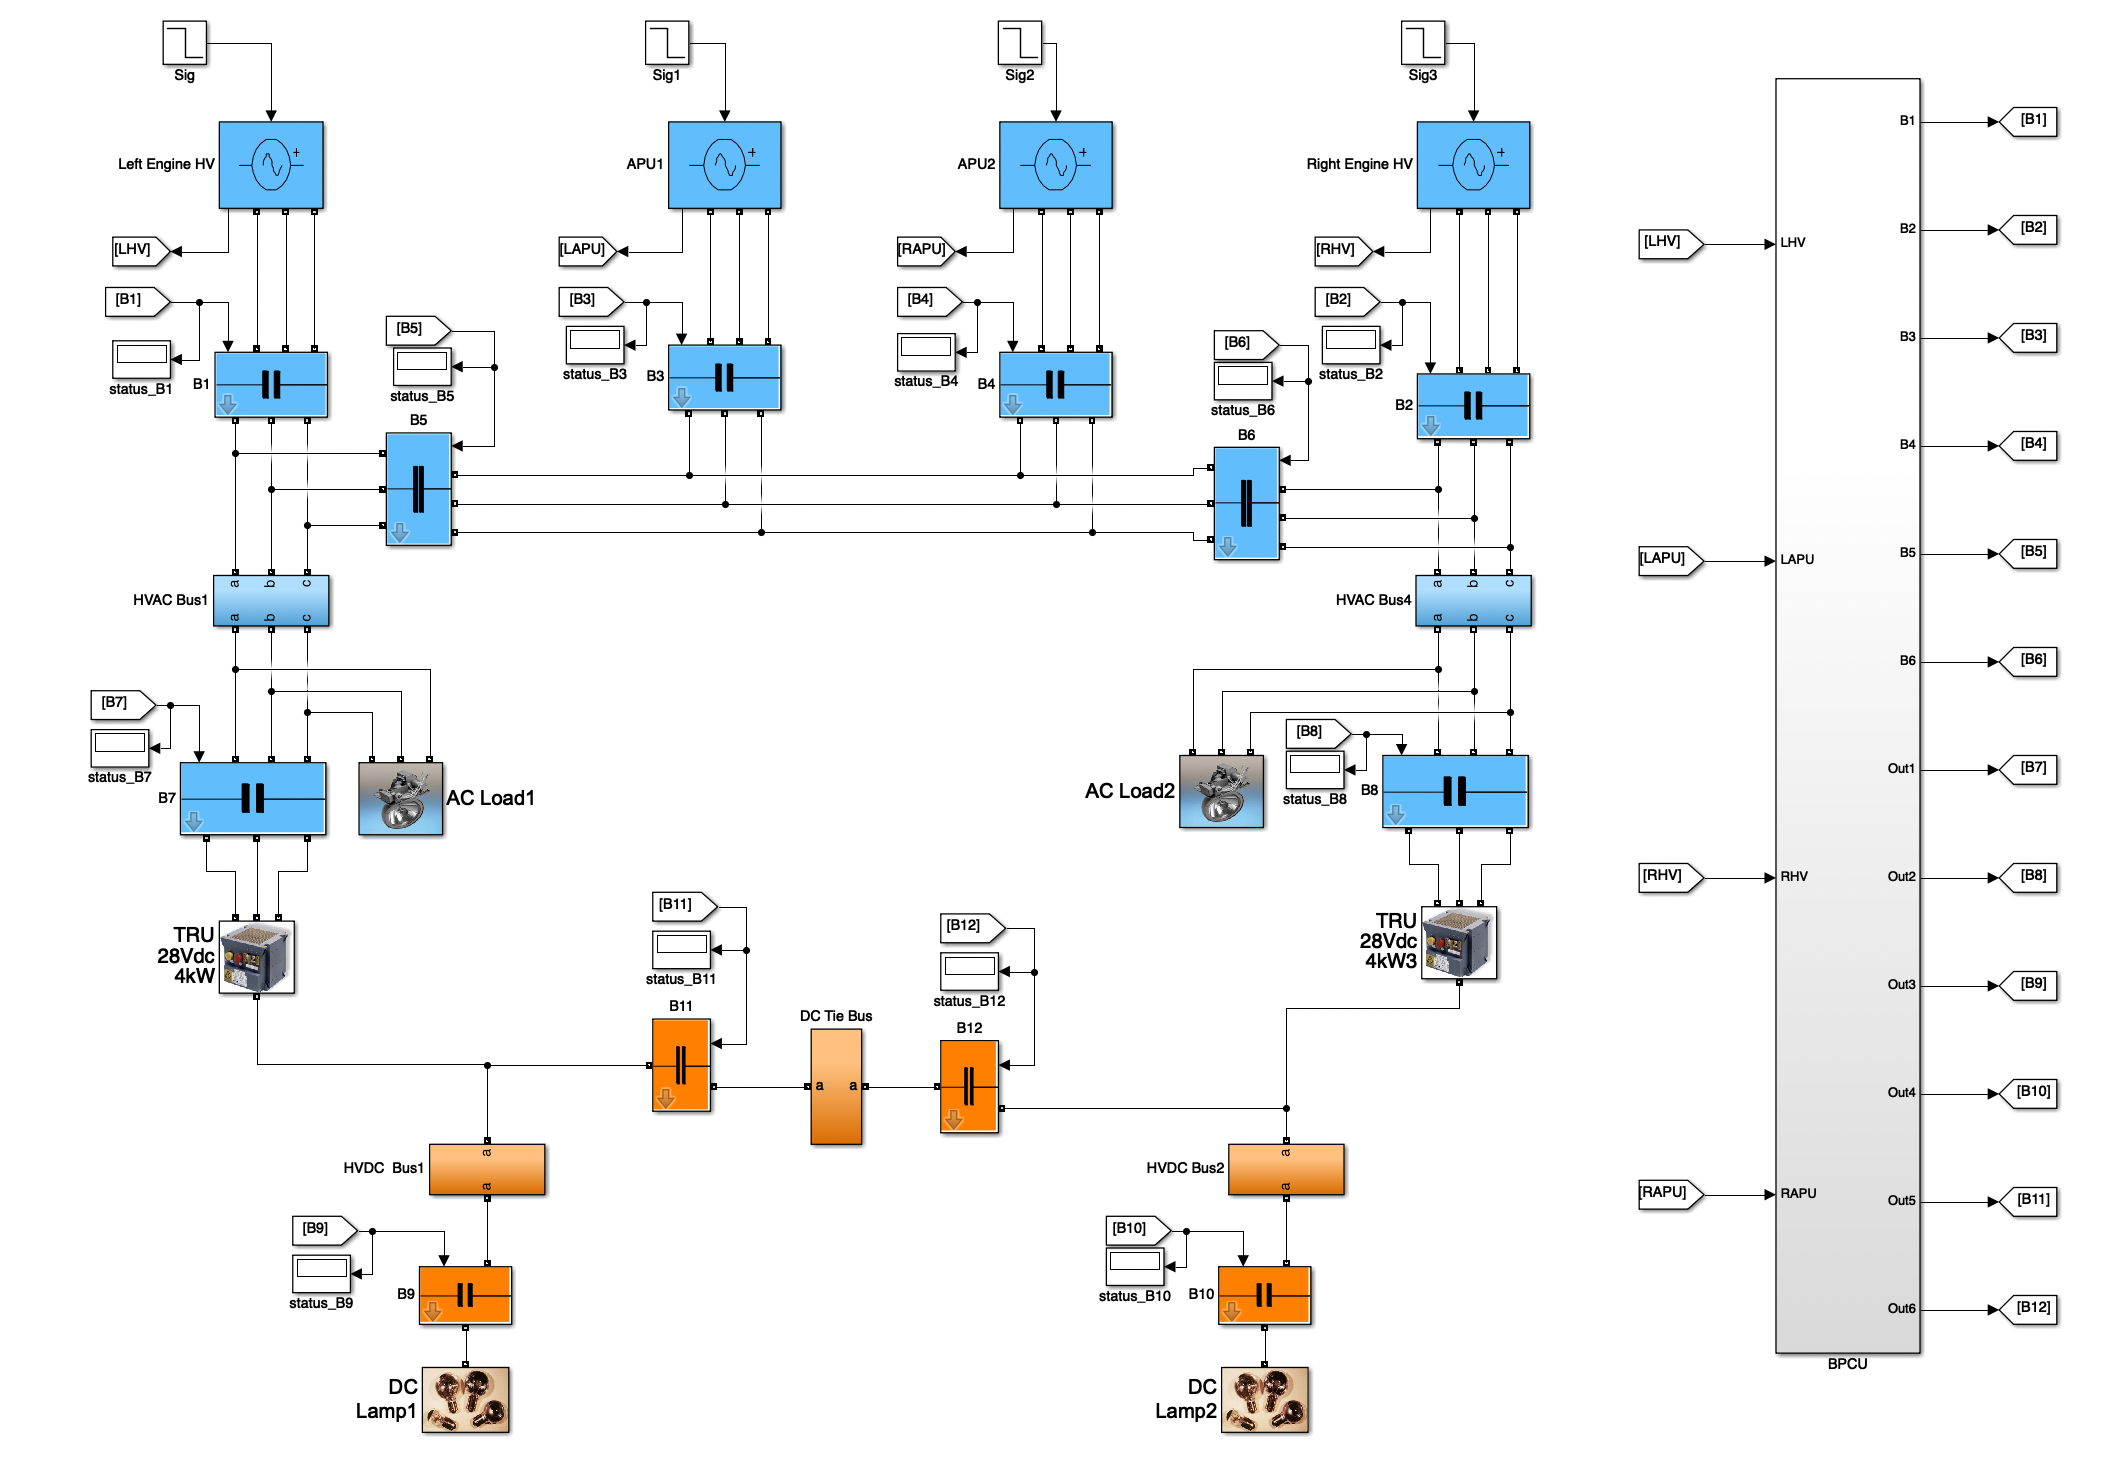
\includegraphics[width=15cm]{fig1.png}
\end{center}
\begin{center}
\small{Figure 1.  An Aircraft Electrical Power System (EPS)}
\end{center}
As Fig. 1 shows, the aircraft EPS is consisted of a set of generators (GL and GR),  auxiliary power units (AL and AR),  power switches (B1 to B12),  rectifier units (HVAC and HVDC), and loads (AC and DC loads). Under some situations (these are specified as environment assumptions), the power generators might malfunction, and auxiliary power units should be connected with loads to ensure that they are always powered and the aircraft stays safe. 
\\ 
\\
BPCU is used to control the buses between power supply and loads when such crisis happens. When the system detects some unexpected power generator malfunction, BPCU controls the power switches to be on or off to connect the healthy power supply with loads. The objective of BPCU is specified by 8 guarantees and our design is based on these 8 guarantees.

\subsection{BPCU Guarantees Interpretation}
Our BPCU control logic is based on 8 guarantees, here is the interpretation of them.
\begin{itemize}
\item \textbf{G1}: This means B1 to B12 are on during the start-up phase.
\item \textbf{G2}: This means B1 and B2 are on but B5 and B6 are off when GL, GR are working.
\item \textbf{G3}: We must control B1 to B6 to prevent paralleled AC power sources connection.
\item \textbf{G4}: This means AL and AR can not be used in parallel,  so when B3 is open, B4 is off; when B4 is open, B3 is off.
\item \textbf{G5}: We must control B1 to B6 to ensure AC buses are empowered.
\item \textbf{G6}: We must control B1 to B6 to ensure DC buses are empowered.
\item \textbf{G7}: This means the leftmost healthy power supply empowers the left AC bus. For example, if GL and AL are healthy, GL empowers the left AC bus; if AL and AR are healthy, AL empowers the left AC bus.
\item \textbf{G8}: This means the rightmost healthy power supply empowers the right AC bus. For example, if GL and AL are healthy, AL empowers the right AC bus; if AL and AR are healthy, AR empowers the right AC bus.
\end{itemize}

\subsection{BPCU Control Logic and Implementation}
\begin{center}
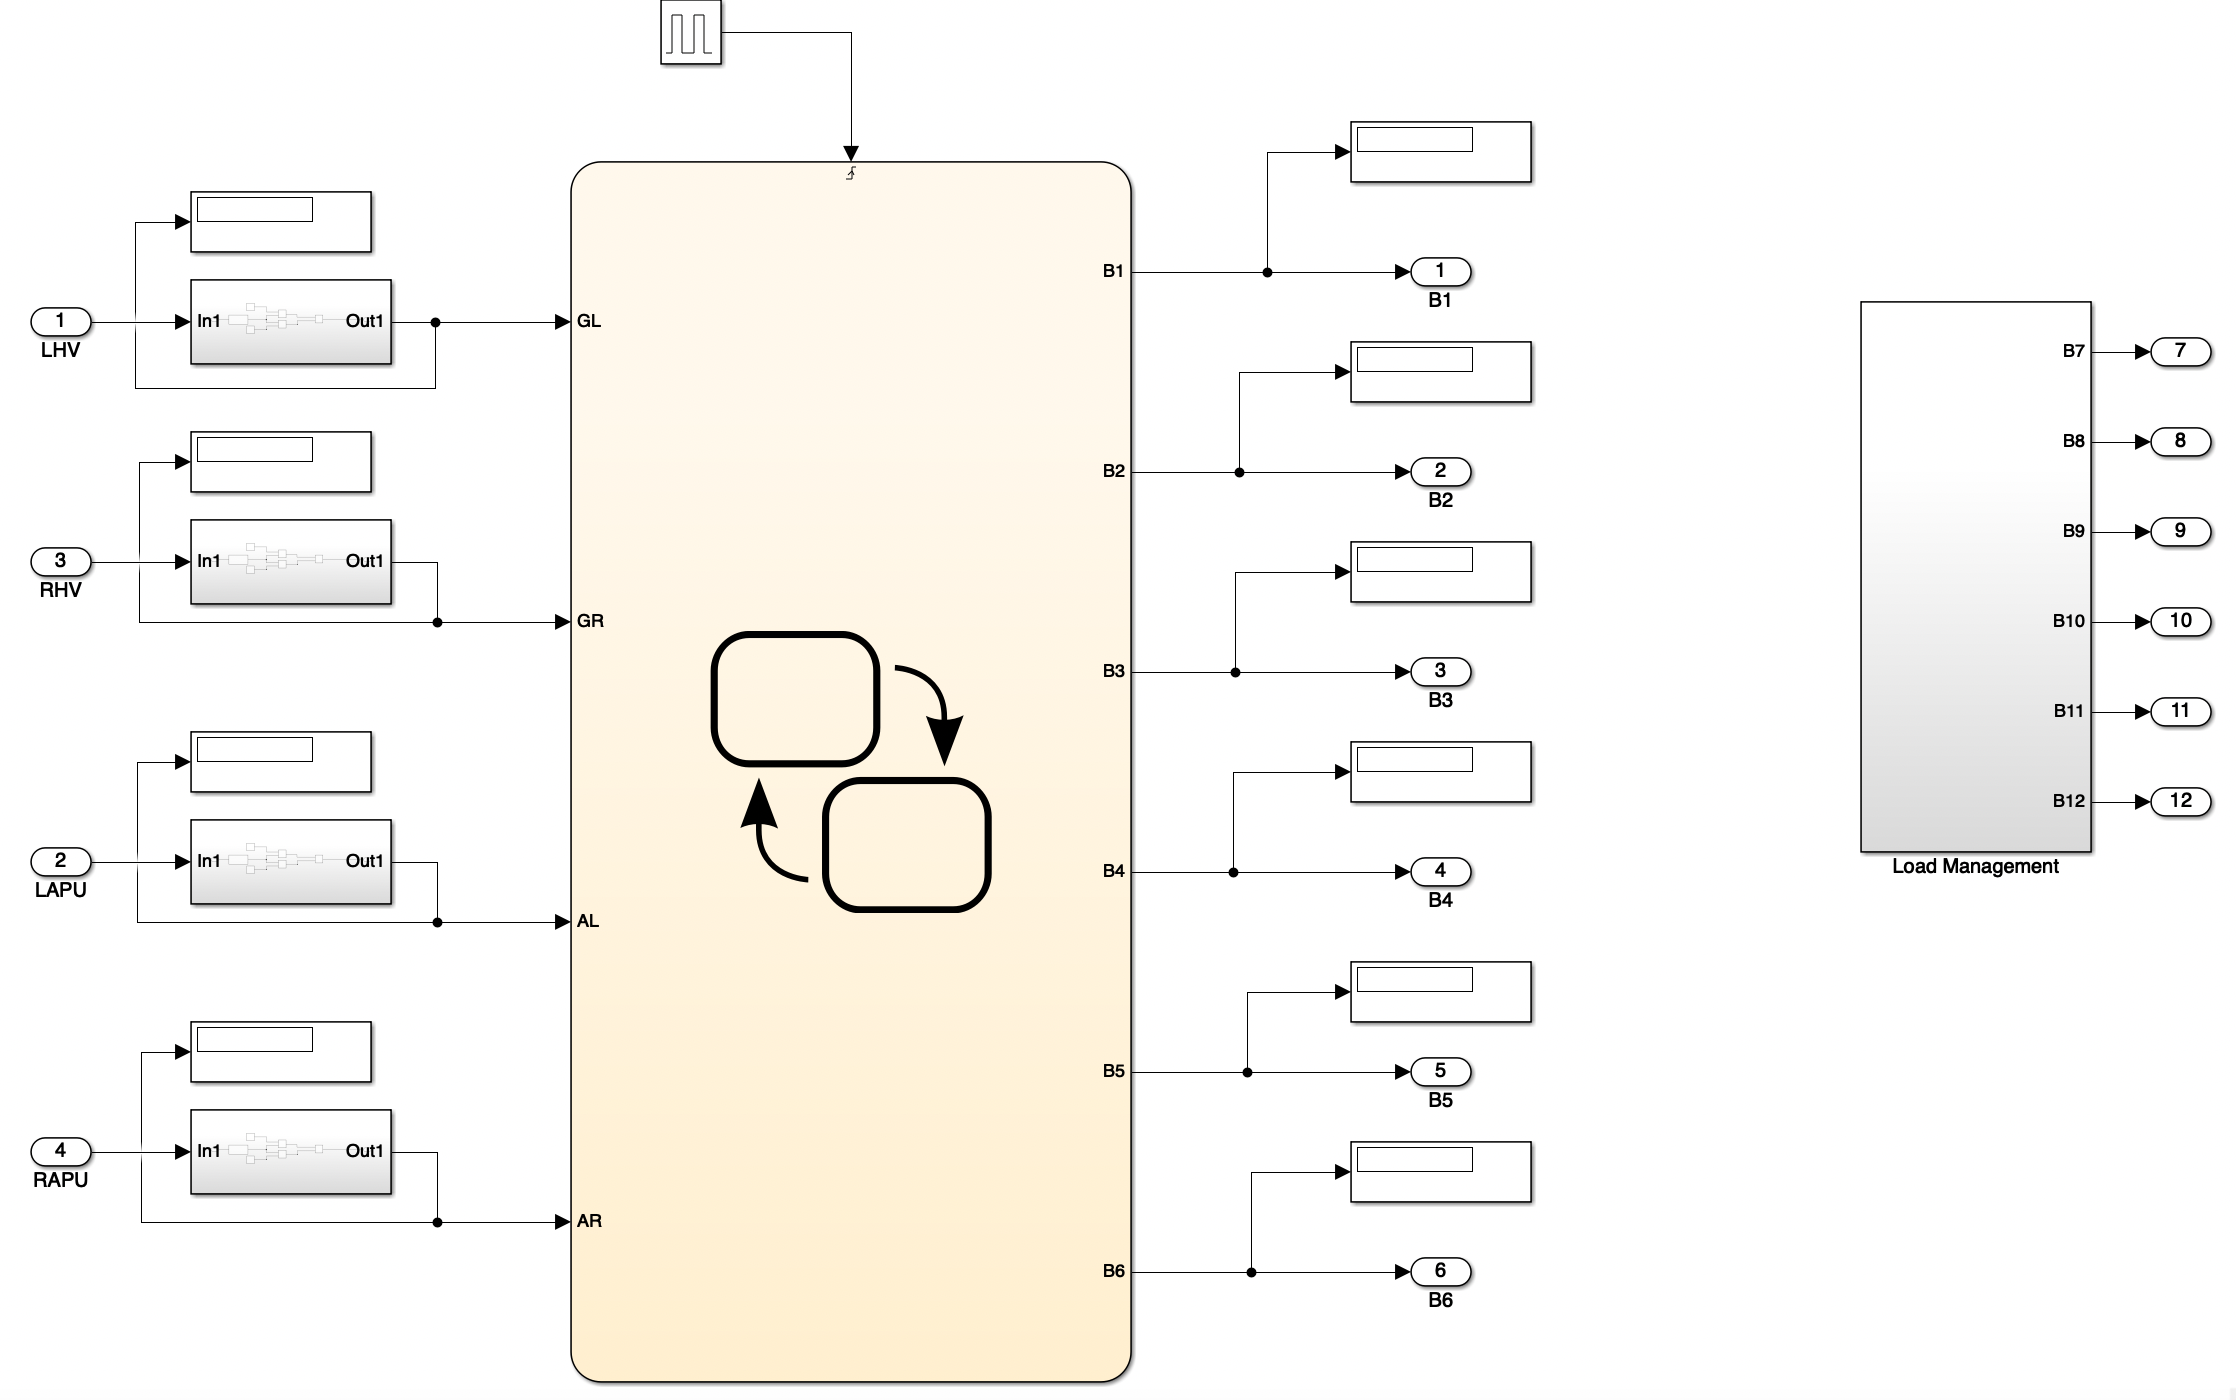
\includegraphics[width=15cm]{fig2.png}
\end{center}
\begin{center}
\small{Figure 2.  BPCU Overview}
\end{center}
Our BPCU is implemented by Stateflow, a graphical and programmable state machine toolbox in Simulink.  Before we introduce its control logic, we first give an overview of our BPCU.
\\
\\
Fig.2 shows the layout of our BPCU. On the left side there are LHV, RHV, LAPU, RAPU signals that represent power supply.  Since there is an environment assumption which states that "an AC bus is correctly powered if the root-mean-square (RMS) voltage at its loads is between 110 V and 120 V and the frequency is 400 Hz",  so the controller switches at a rate of 2.5 ms and a voltage monitor is used to ensure that the RMS voltage is within the desired range (see Fig.3 below).
\begin{center}
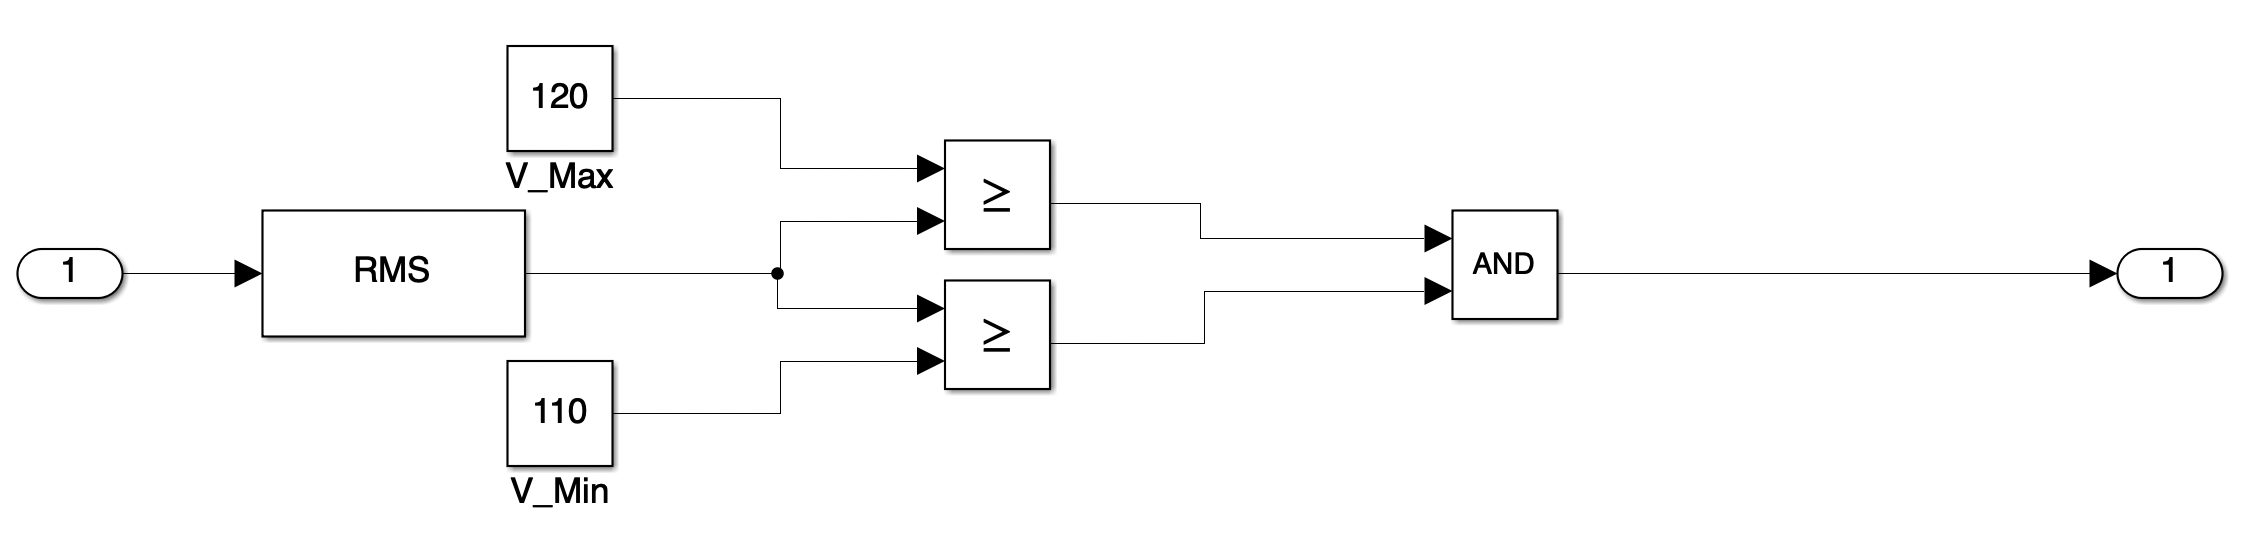
\includegraphics[width=13cm]{fig3.png}
\end{center}
\begin{center}
\small{Figure 3.  The Voltage Monitor Module}
\end{center}
On the right side of Fig.2 are the output signals generated by the controller. The controller is visualized in Fig. 4.
\begin{center}
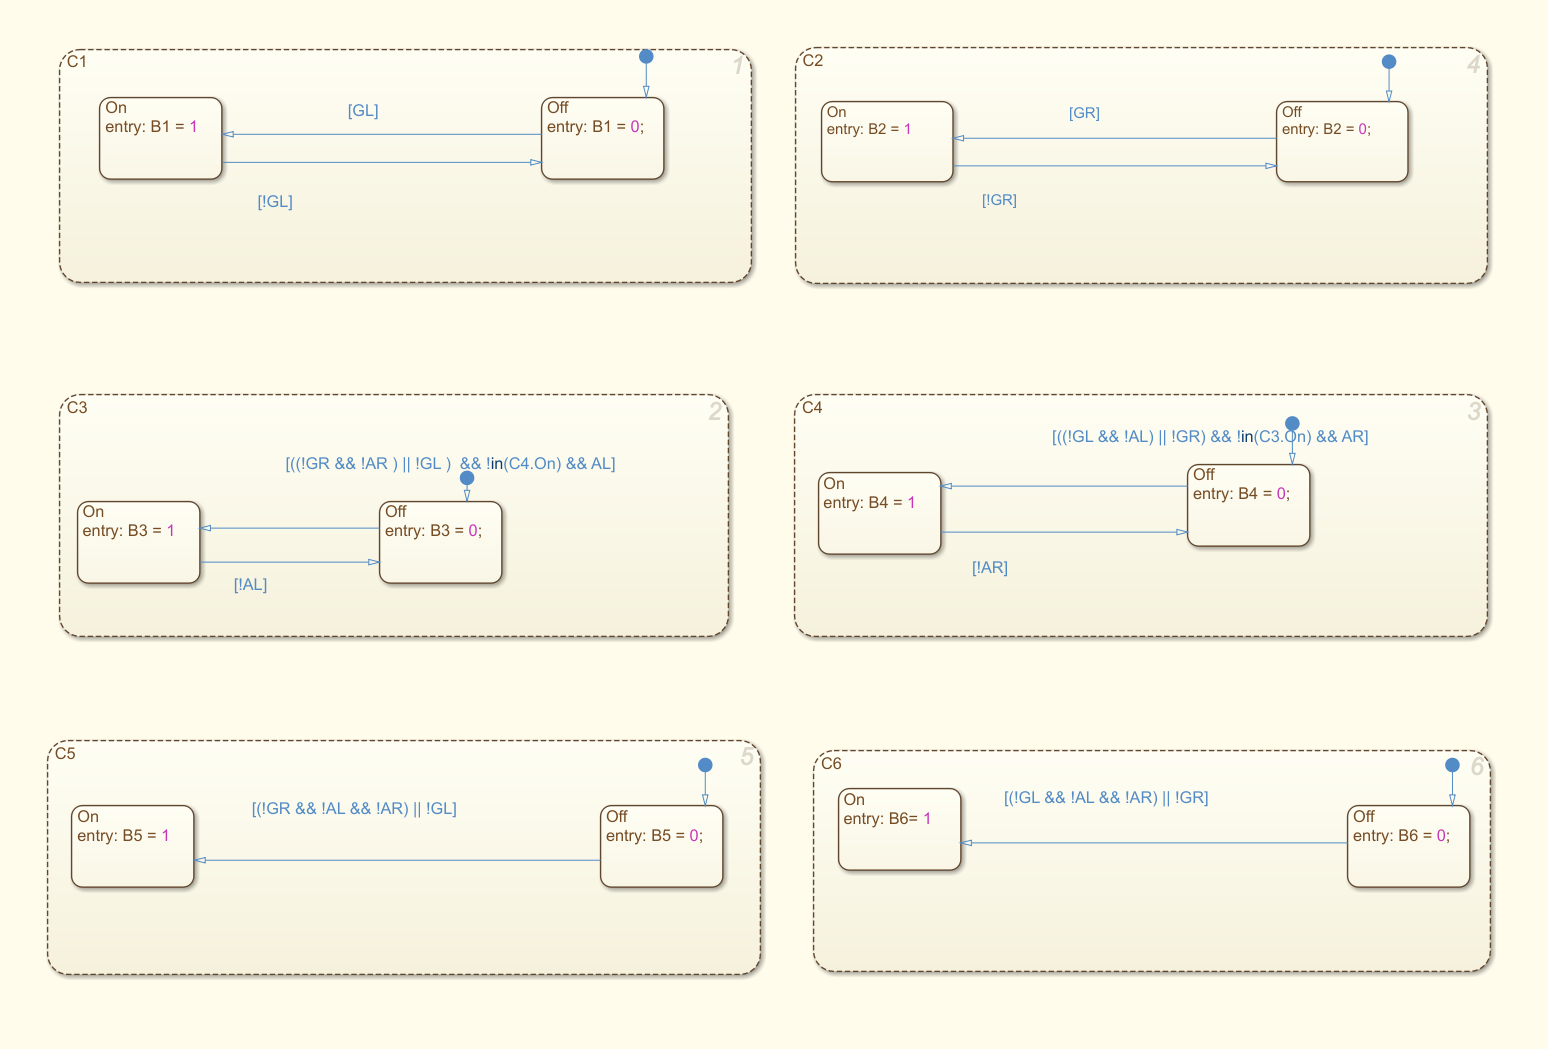
\includegraphics[width=14.25cm]{fig4.png}
\end{center}
\begin{center}
\small{Figure 4.  The Controller}
\end{center}
There are 6 modules that control B1 to B6.
\begin{itemize}
\item \textbf{C1}: B1 changes from 0 to 1 when $GL$,  B1 changes from 1 to 0 when $!GL$, because if GL functions well B1 is open to power the left AC bus.
\item \textbf{C2}: B2 changes from 0 to 1 when $GR$,  B2 changes from 1 to 0 when $!GR$, because if GR functions well B2 is open to power the right AC bus.
\item \textbf{C3}: B3 changes from 0 to 1 when $!AL$,  B3 changes from 1 to 0 when \\$((!GR \&\& !AR) || !GL) \&\& !C4\&\& AL$, because B3 is open when (1) AL functions well; (2) B4 is off since B3 and B4 cannot be open at the same time because of G4; (3) GL is not working so AL empowers the left AC bus, or GR and AR are both not working so AL empowers the right AC bus.
\item \textbf{C4}:  B4 changes from 0 to 1 when $!AR$,  B4 changes from 1 to 0 when \\$((!GL \&\& !AL) || !GR) \&\& !C3 \&\& AR$, because B4 is open when (1) AR functions well; (2) B3 is off since B3 and B4 cannot be open at the same time because of G4; (3) GR is not working so AR empowers the right AC bus, or GL and AL are both not working so AR empowers the left AC bus.
\item \textbf{C5}: B5 changes from 0 to 1 when $((!GR \&\& !AL \&\& !AR) || !GL)$, because B5 is open when GL is not working so some power supply on the right of GL empowers the left AC bus or GR, AL, and AR are all not working so GL empowers the right AC bus.
\item \textbf{C6}: B6 changes from 0 to 1 when $((!GL \&\& !AL \&\& !AR) || !GR)$, because B6 is open when GR is not working so some power supply on the left of GR empowers the right AC bus or GL, AL, and AR are all not working so GR empowers the left AC bus. 
\end{itemize}
\pagebreak

\section{Simulation Results and Design Verification}

\subsection{General Idea}
In this section, we introduce how to use simulation to verify that our design meets all system guarantees. We have totally 10 cases to consider:
\begin{itemize}
\item \textbf{Case 1}: GR, GL are working 
\item \textbf{Case 2}: GR is not working
\item \textbf{Case 3}: GL is not working
\item \textbf{Case 4}: GR, AR are not working
\item \textbf{Case 5}: GL, AL are not working
\item \textbf{Case 6}: GR, GL are not working 
\item \textbf{Case 7}: GR, GL, AR are not working 
\item \textbf{Case 8}: GR, GL, AL are not working 
\item \textbf{Case 9}: GR, AR, AL are not working 
\item \textbf{Case 10}: GL, AR, AL are not working 
\end{itemize}
The basic case is that the system works well, which means GR and GL are working (regardless of the status of AR and AL). If the basic case gives a desired result, it proves that G2 is satisfied.  
\\
\\
The second and third cases handle the situation when one of GR and GL fails and others are not. Because of G4, G7, G8, only one APU is inserted into the network and the leftmost available APU empowers the left AC bus and the rightmost available APU empowers the right AC bus, the results are definite. For the second case, AR empowers the right AC bus; for the third case, AL empowers the left AC bus.
\\
\\
Based on the second and third cases, the fourth and fifth cases verify if AL empowers the right AC bus if both GR and AR fail, AR empowers the left AC bus if both GL and AL fail.
\\
\\
The rest four cases verify if the system can use only one generator to empower both AC buses. Since there is an environment assumption that states "at least one power source is always healthy", BPCU does not need to handle the case that all generators fail. Finally, G1,  G3, G5, and G6 are proved if all the above cases are satisfied.
\pagebreak

\subsection{Case 1: GR, GL Are Working}
\newlength{\imageheight}
\settowidth{\imageheight}{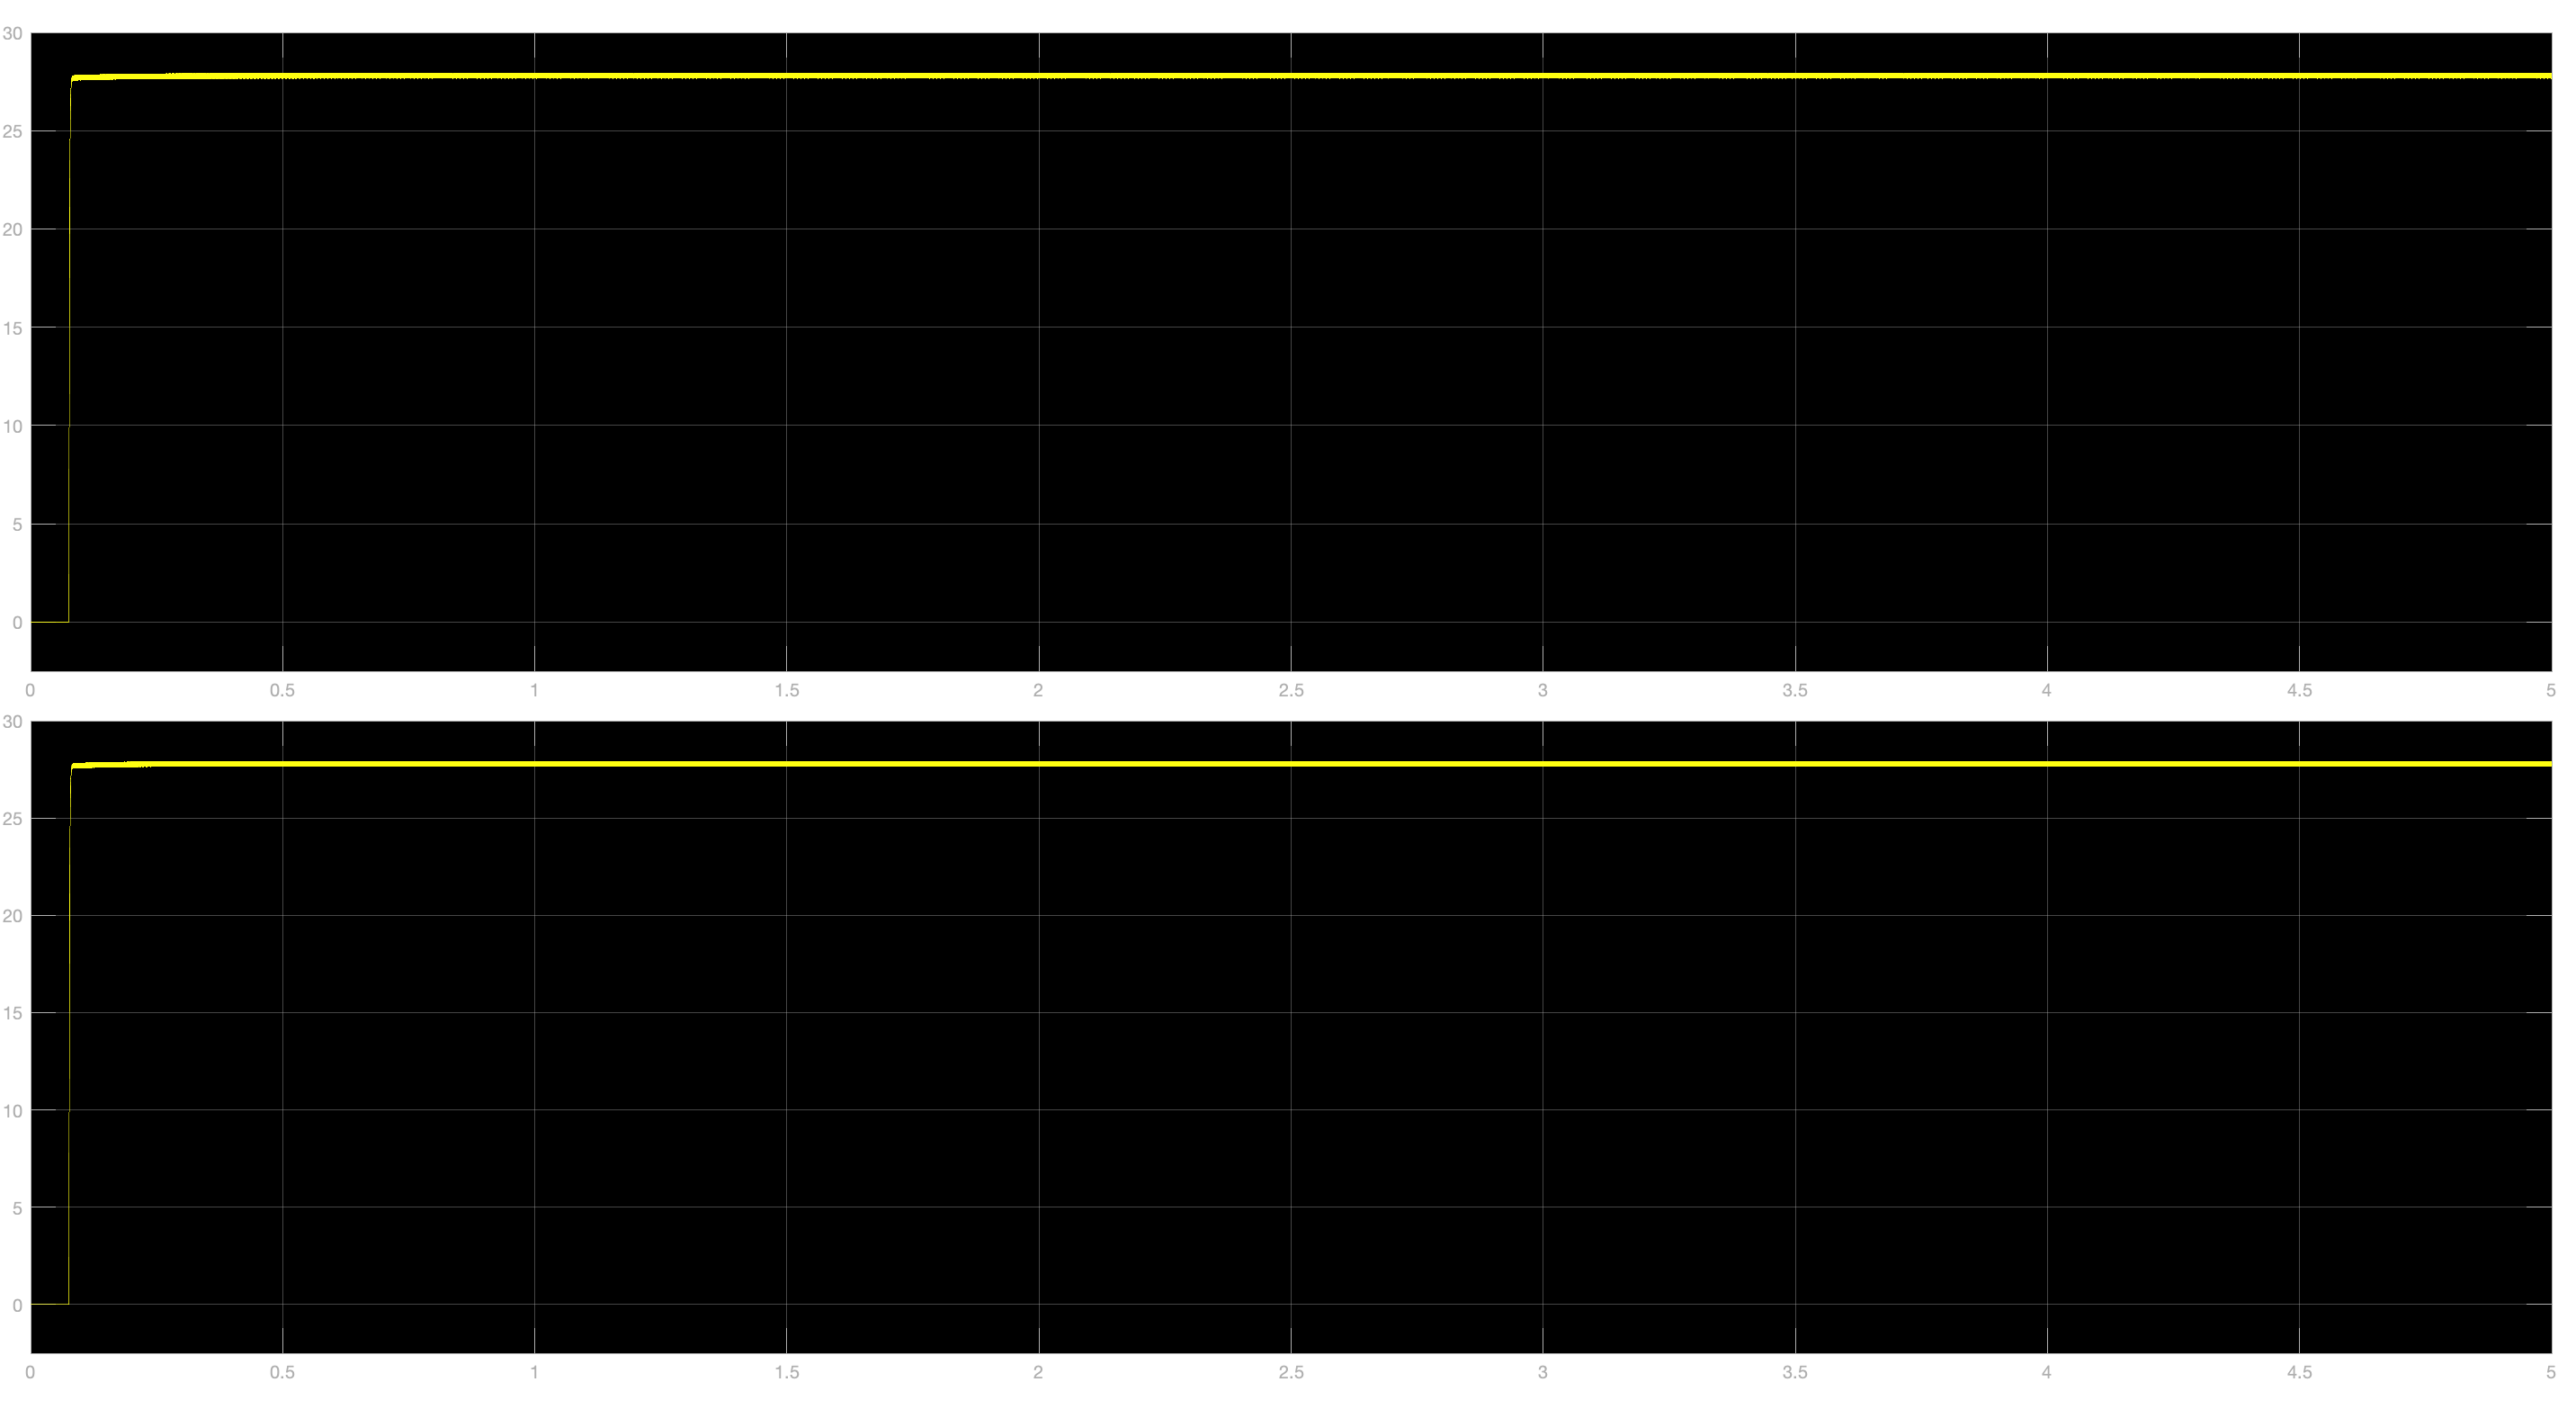
\includegraphics{all_powered_load1.png}}
\begin{center}
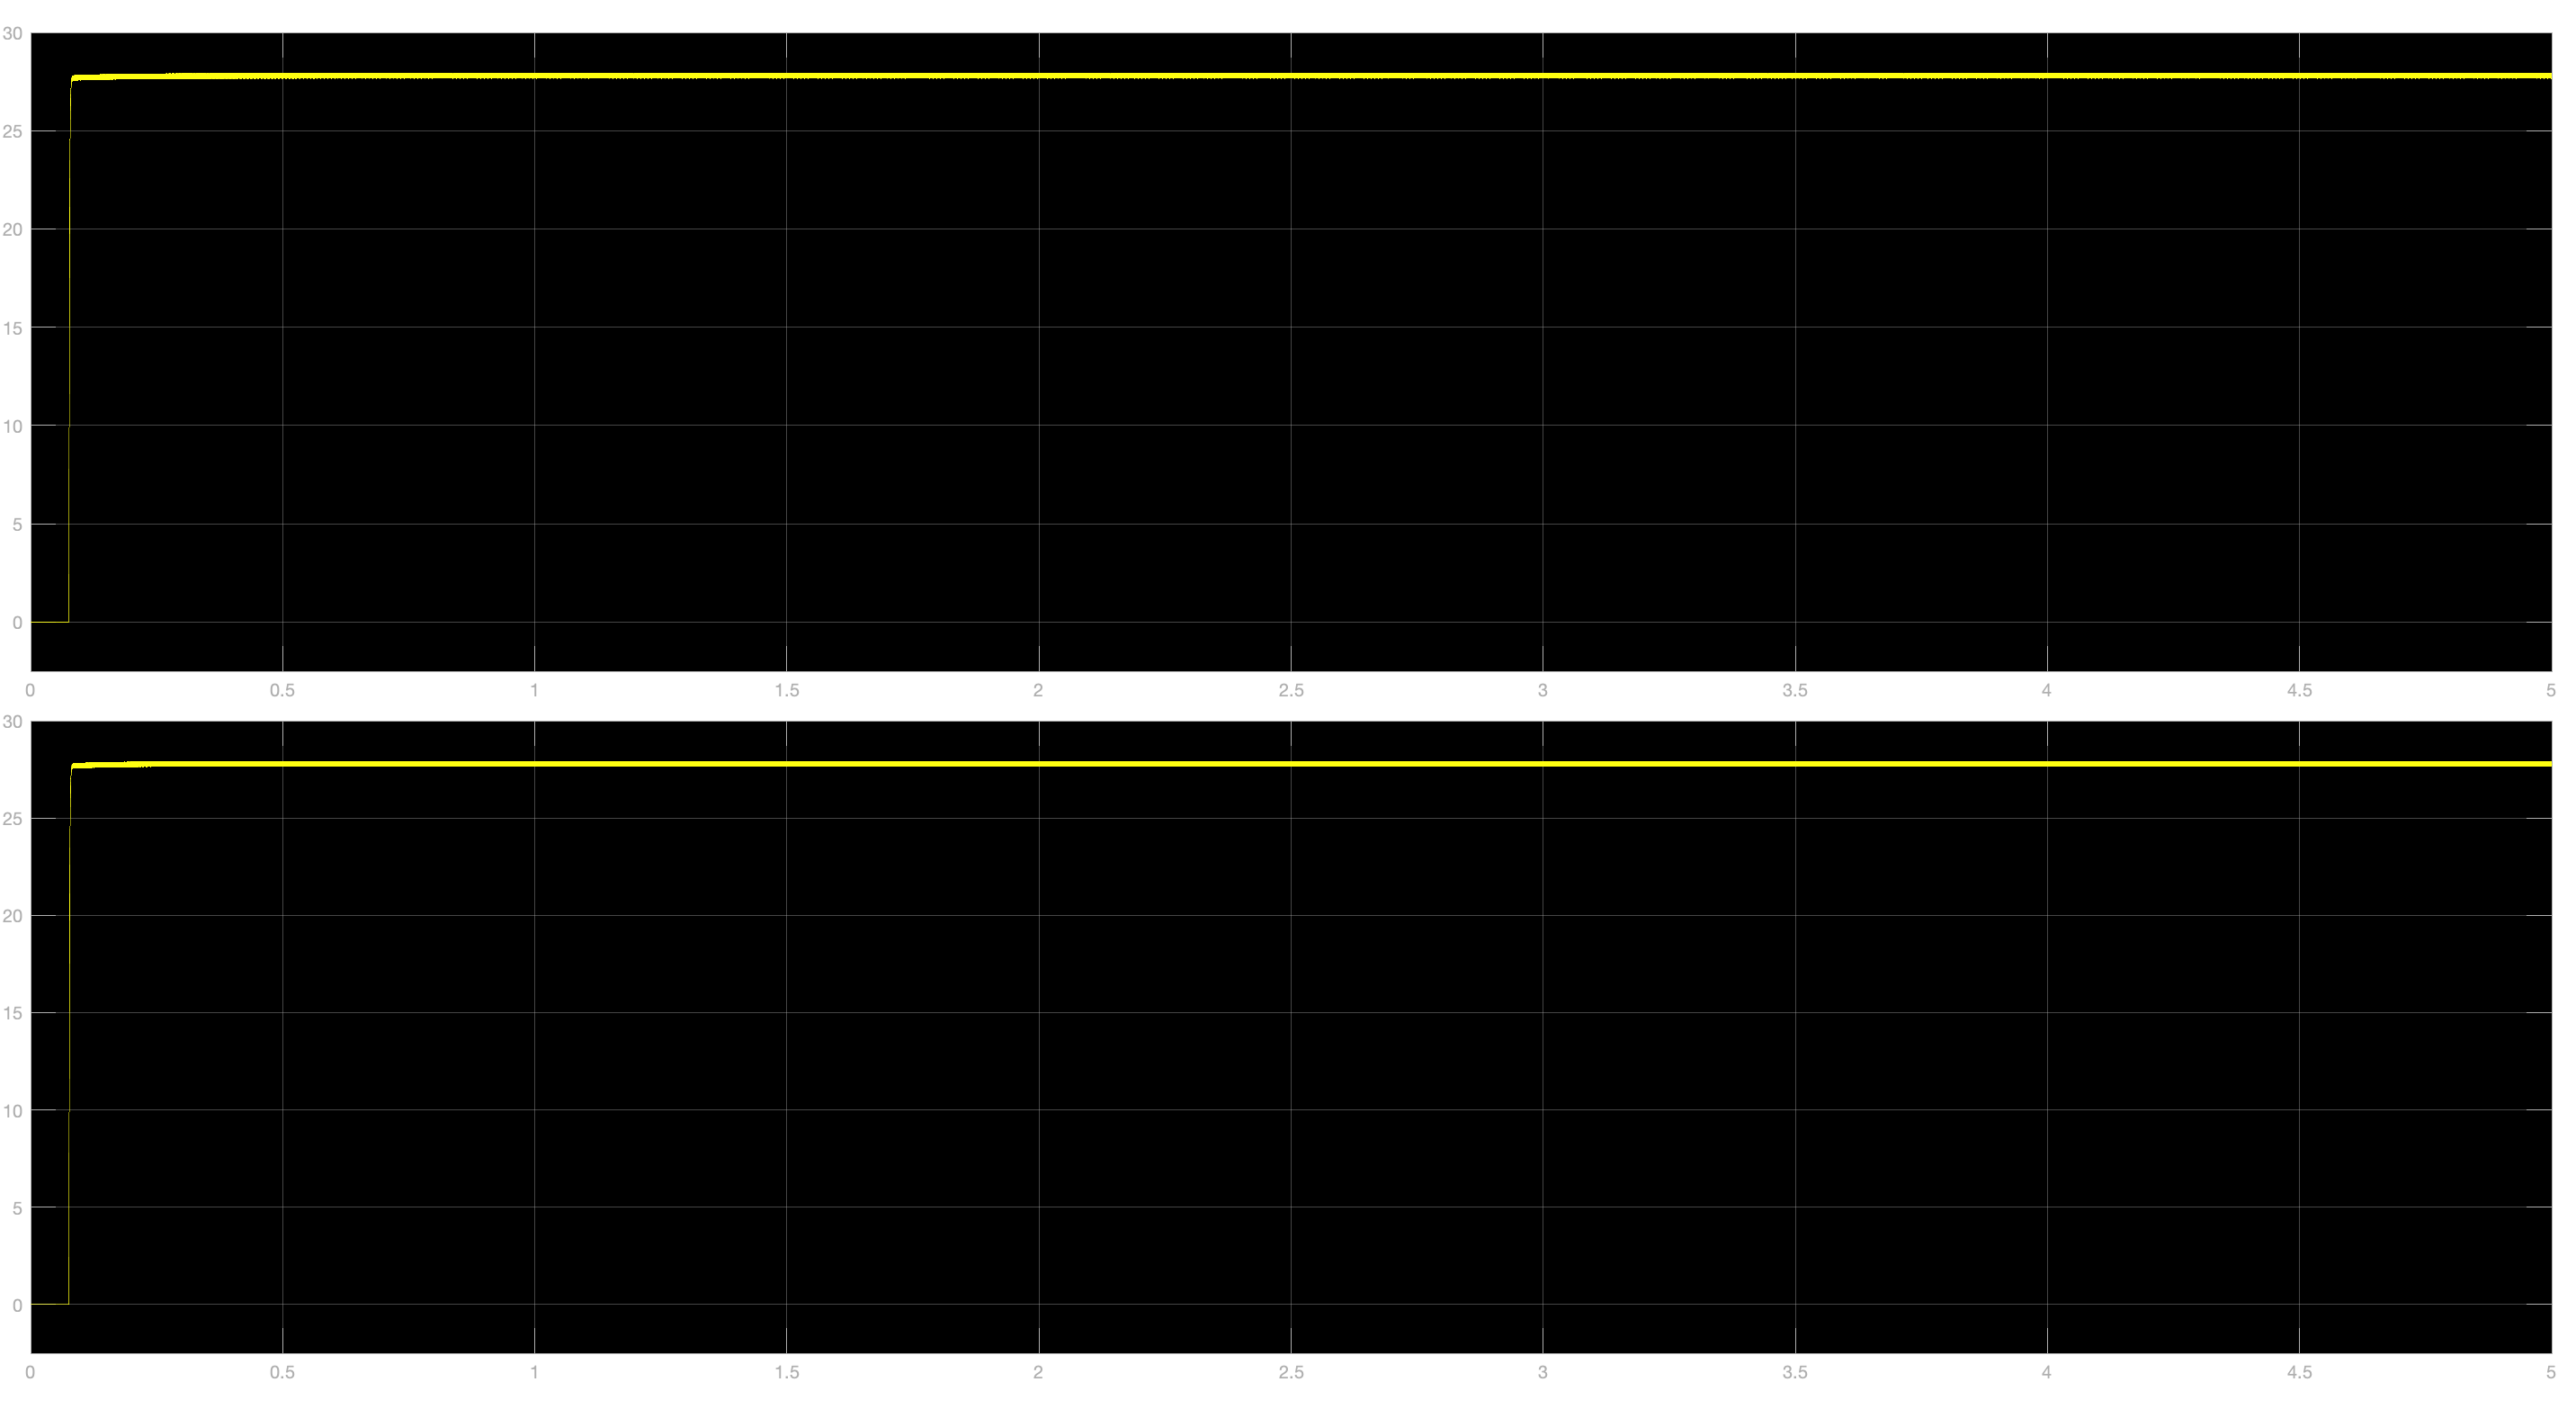
\includegraphics[trim= 0 0.28\imageheight{} 0 0, clip, width = 0.165\imageheight{}]{all_powered_load1.png}
\end{center}
\begin{center}
\small{Figure 2.2.1 Left DC Load Waveform}
\end{center}
\begin{center}
{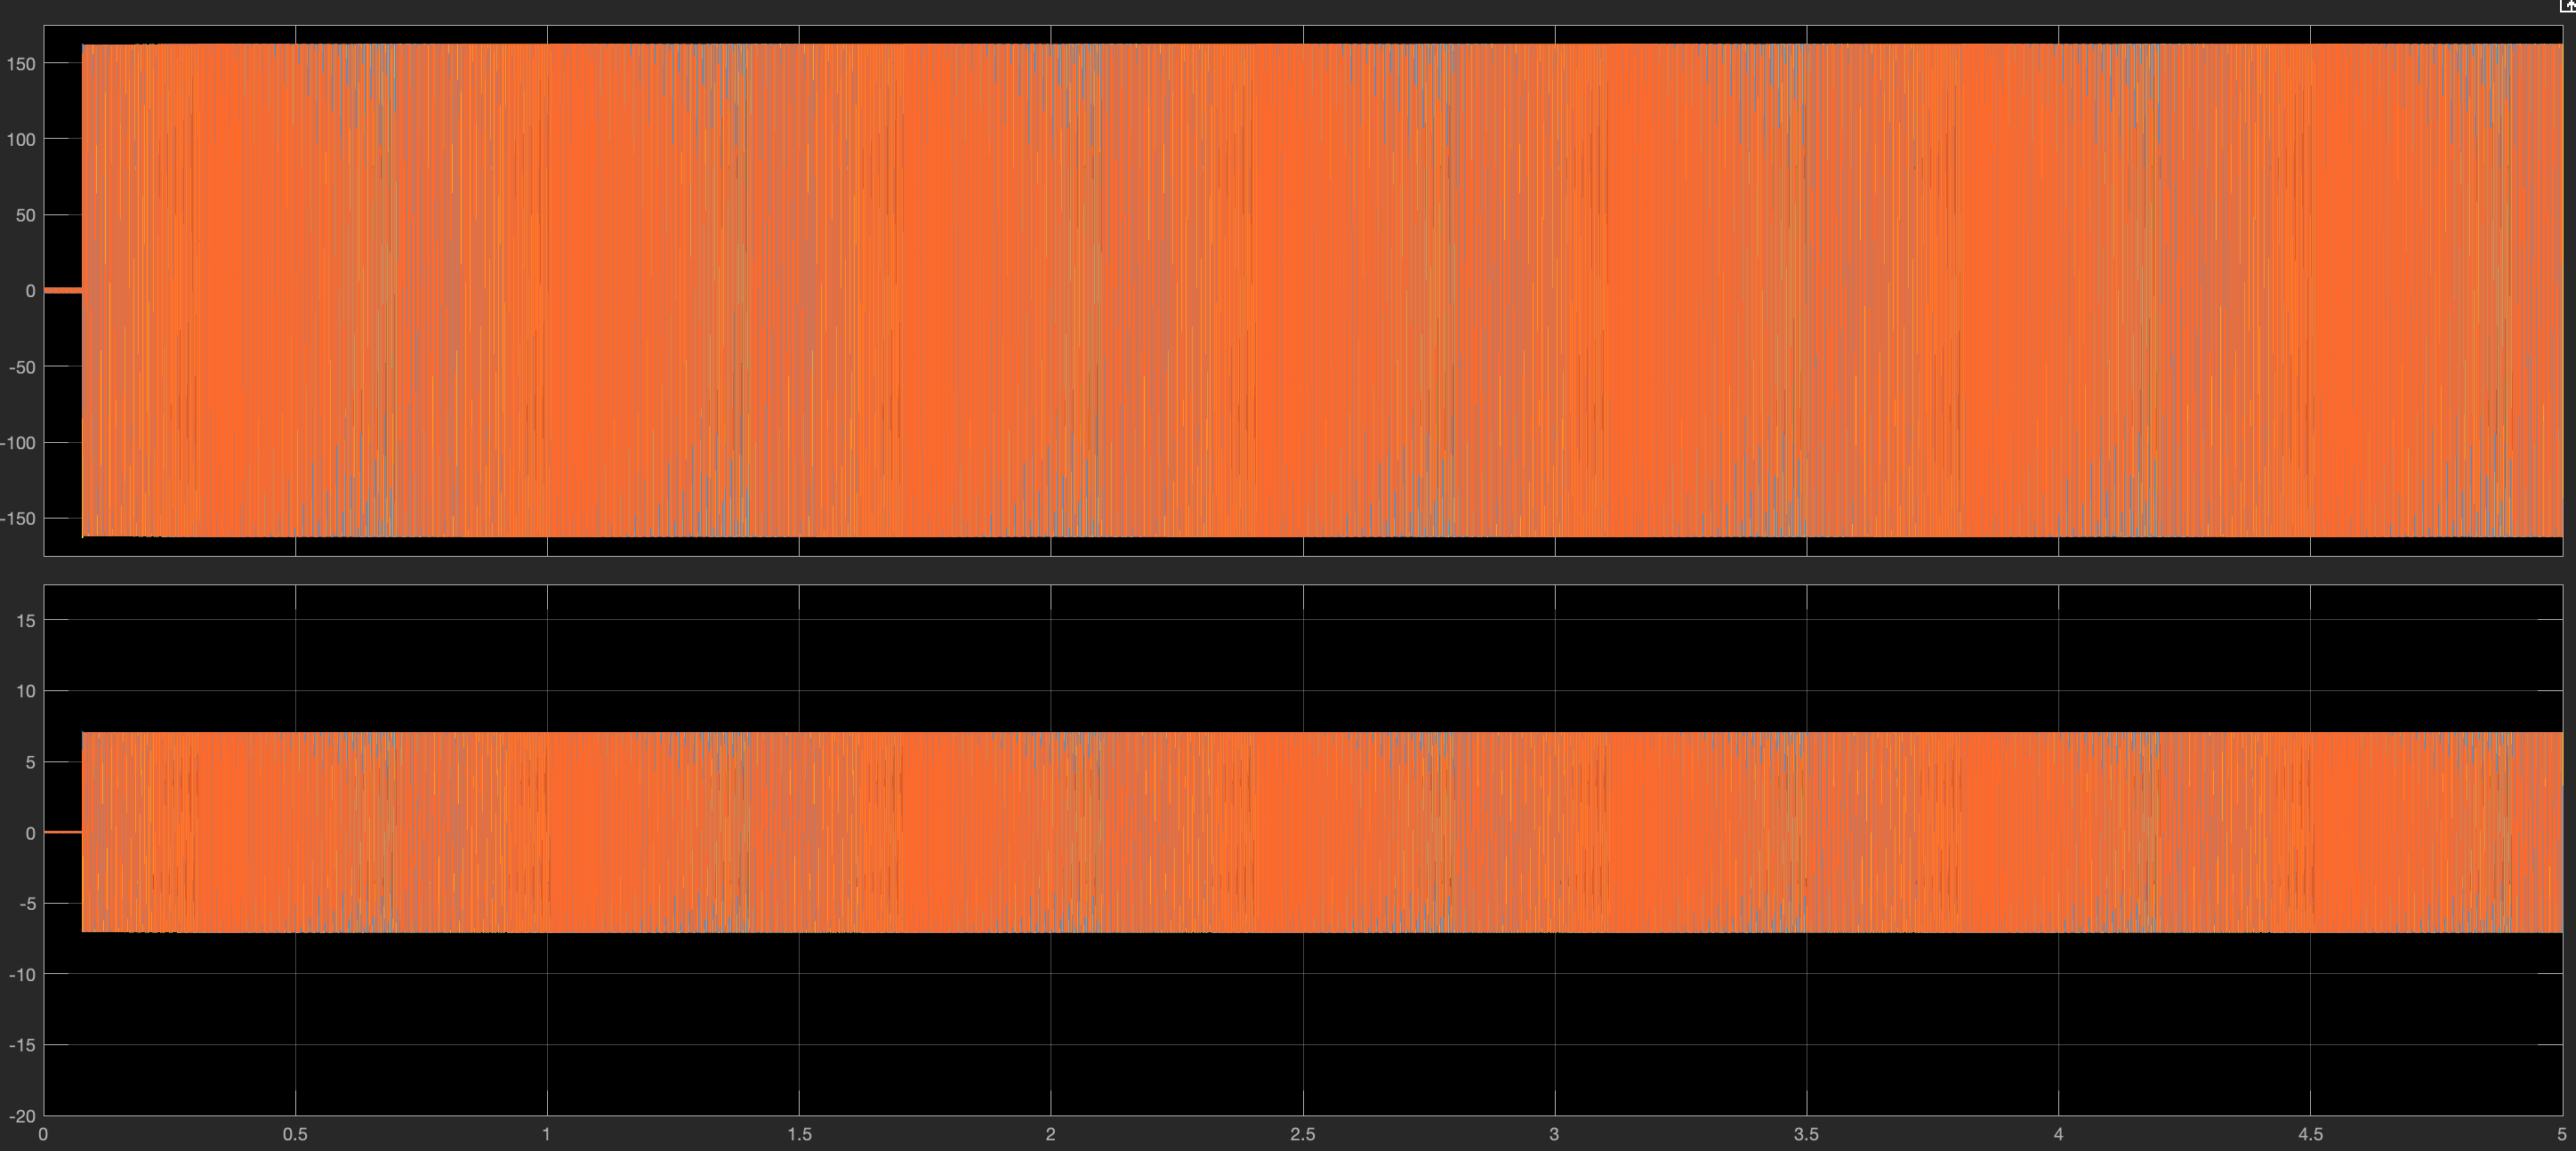
\includegraphics[width=13.5cm]{ac.png}}
\end{center}
\begin{center}
\small{Figure 2.2.2 Left AC Load Waveform}
\end{center}
We include an AC load waveform in this case to show that DC waveform is corresponding to AC waveform, so we just include DC waveforms in the following cases.
\\
\settowidth{\imageheight}{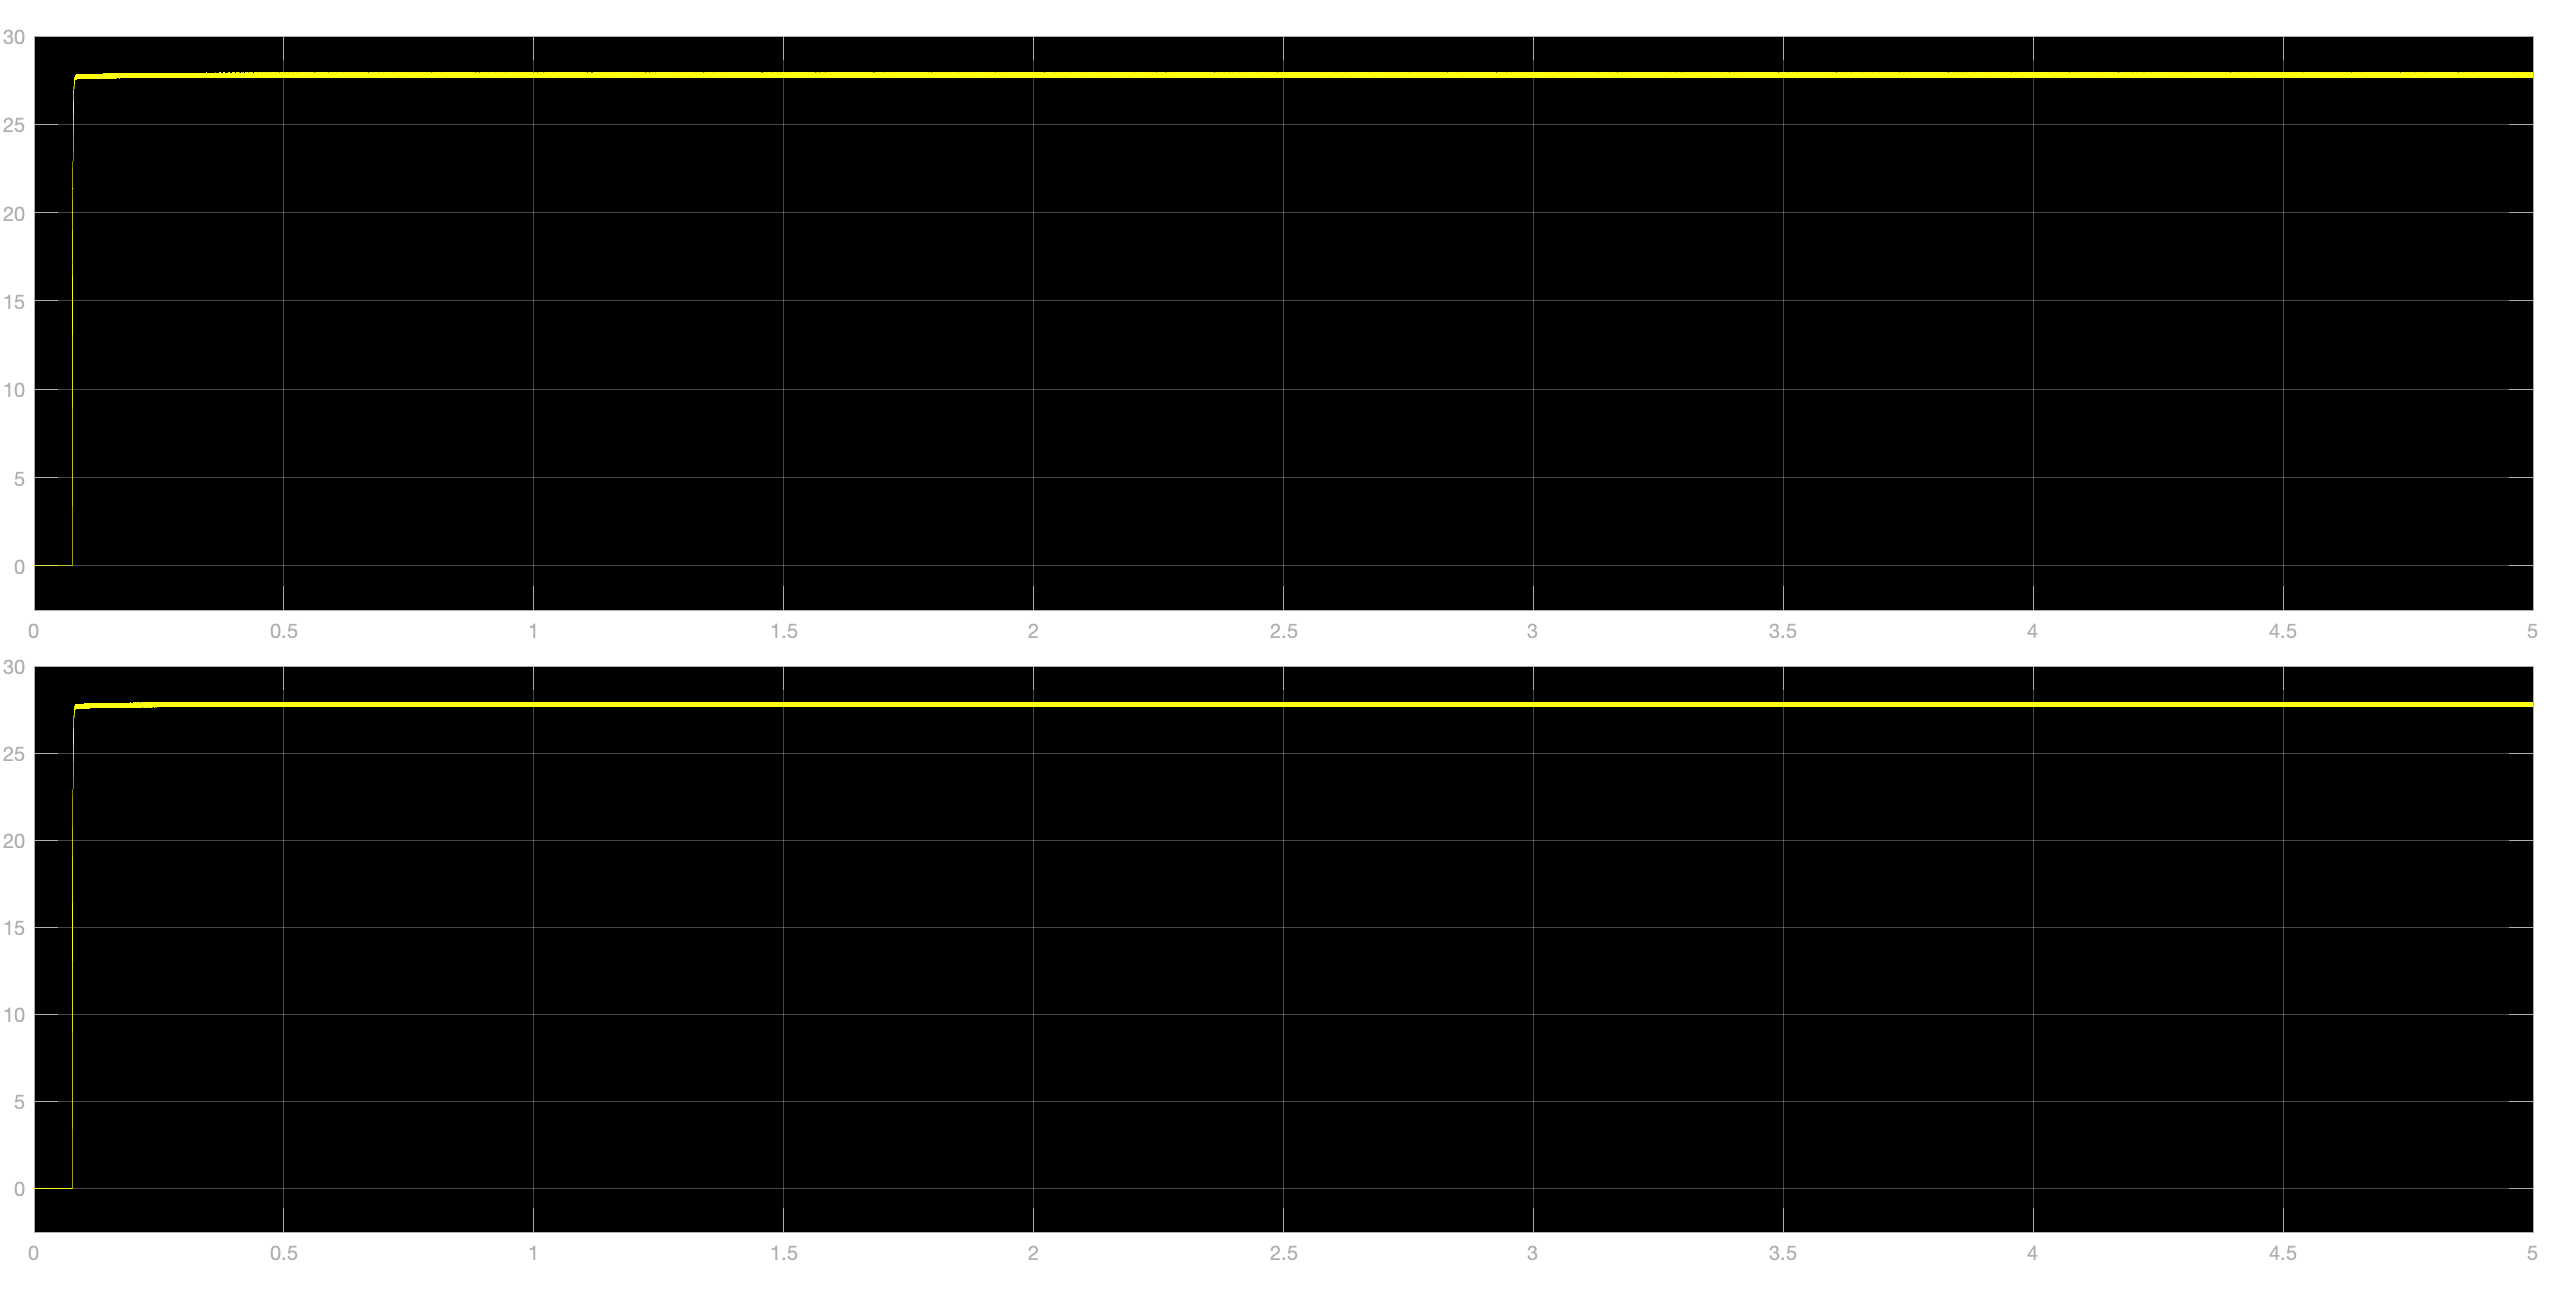
\includegraphics{all_powered_load2.png}}
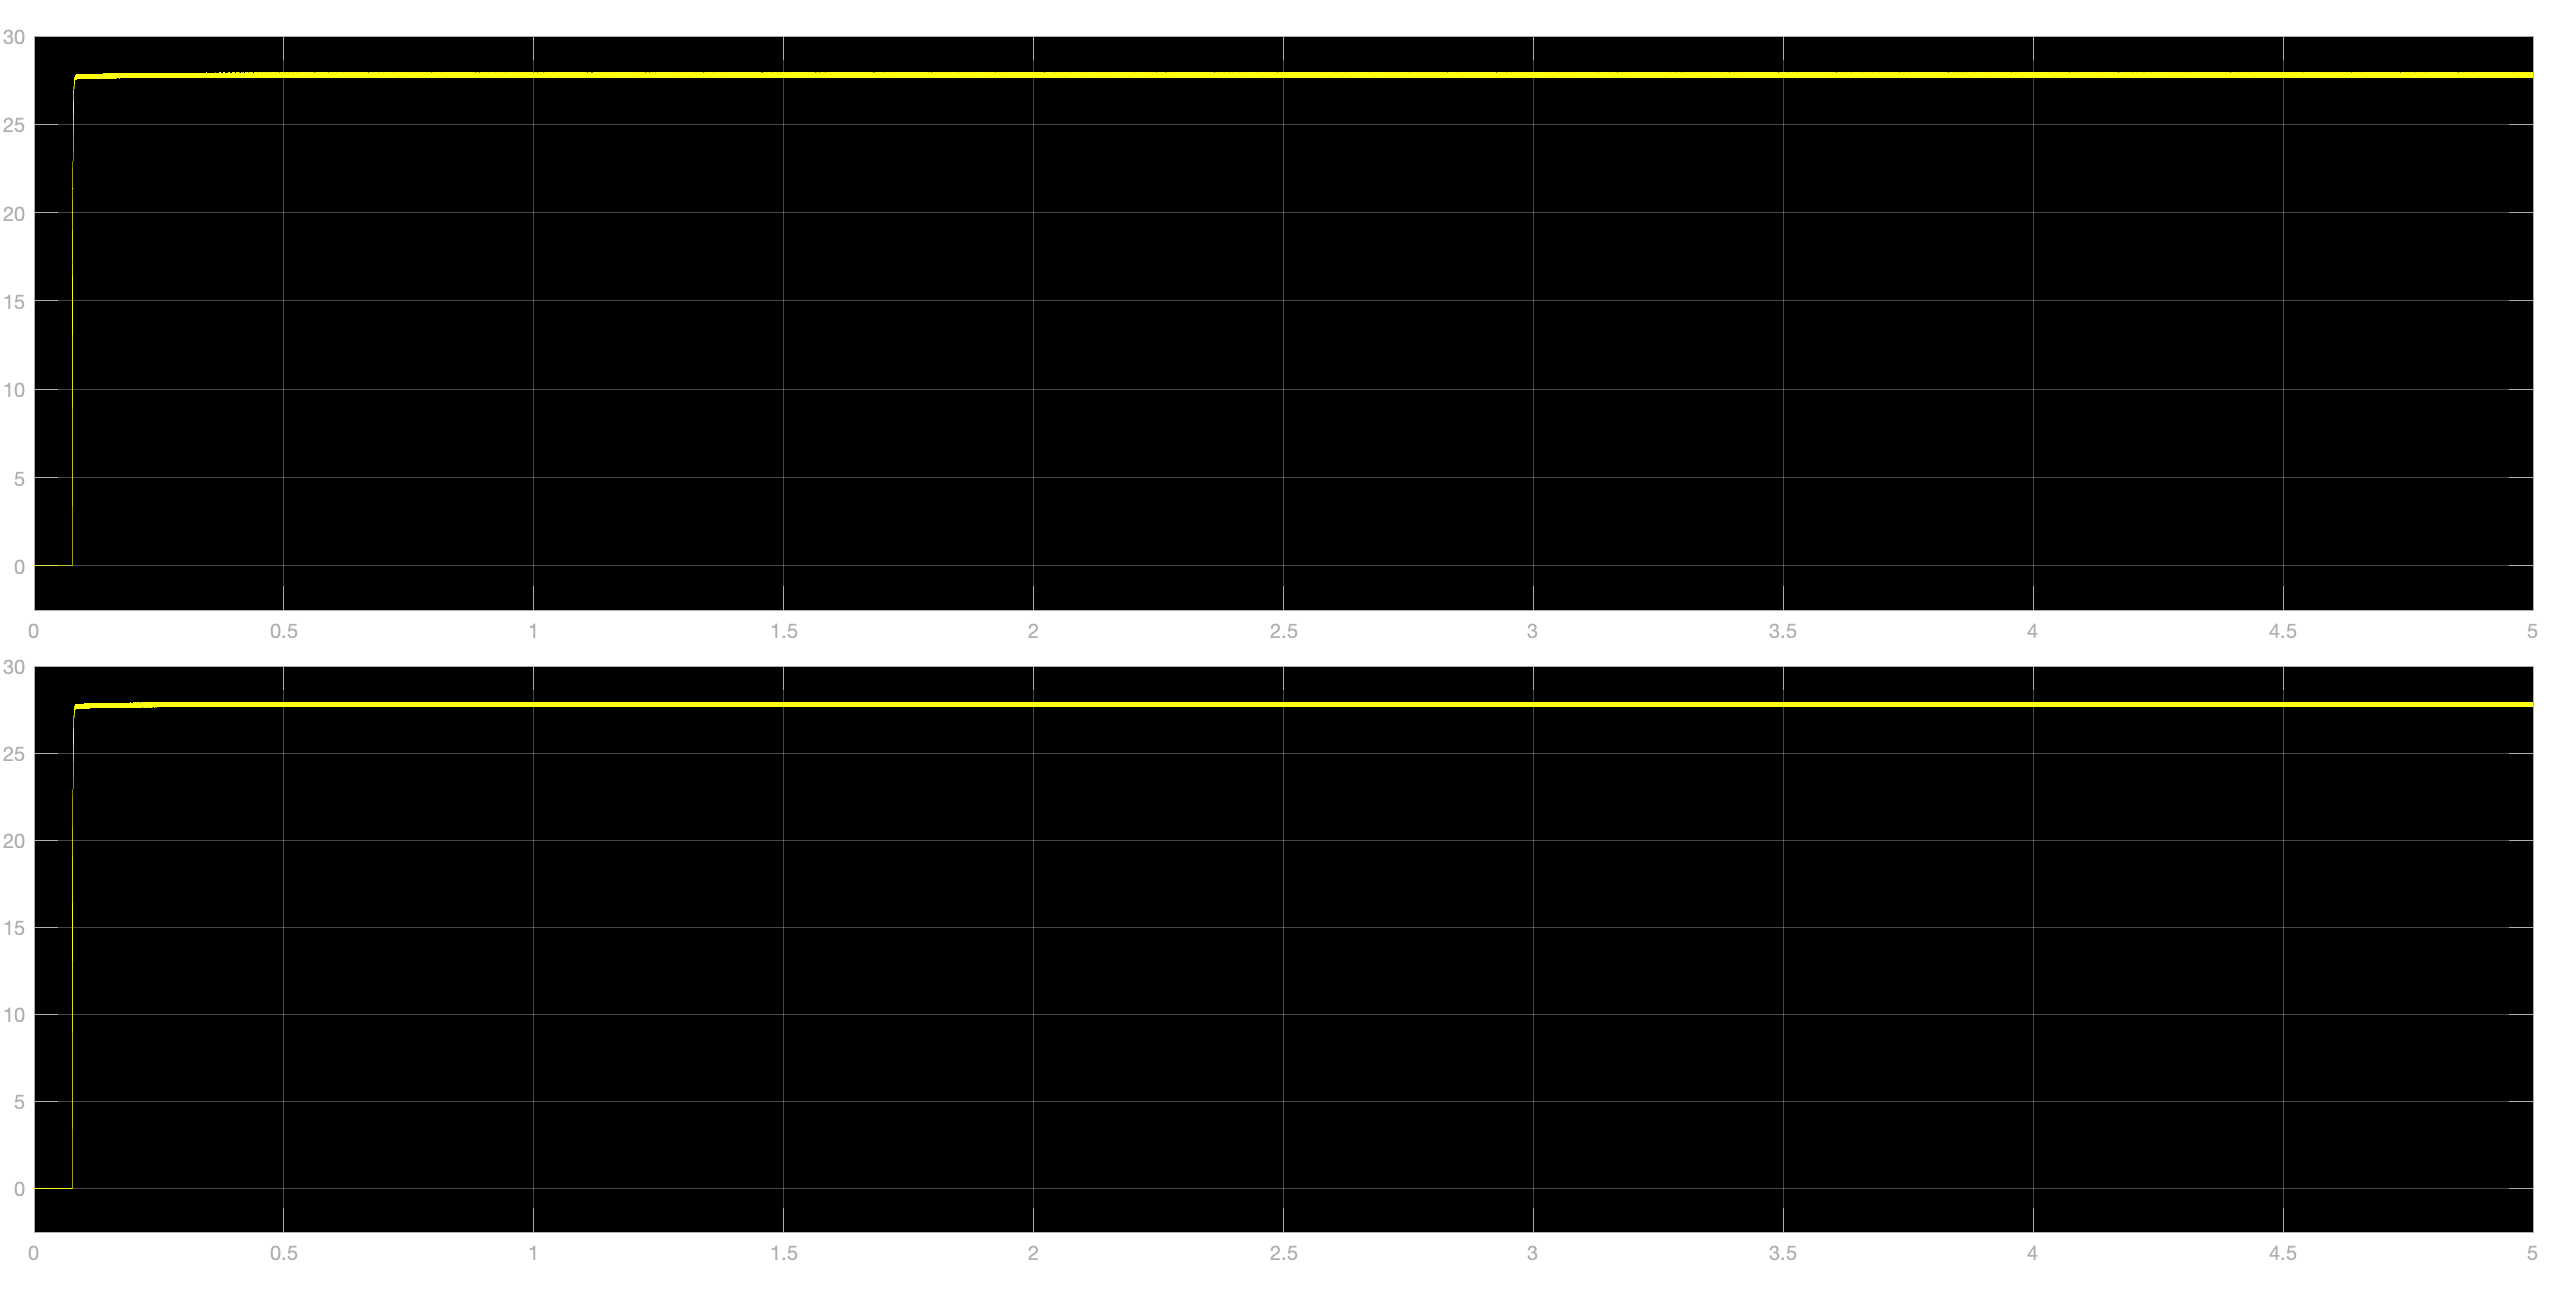
\includegraphics[trim= 0 0.255\imageheight{} 0 0, clip, width = 0.185\imageheight{}]{all_powered_load2.png}
\begin{center}
\small{Figure 2.2.3 Right DC Load Waveform}
\end{center}
\begin{center}
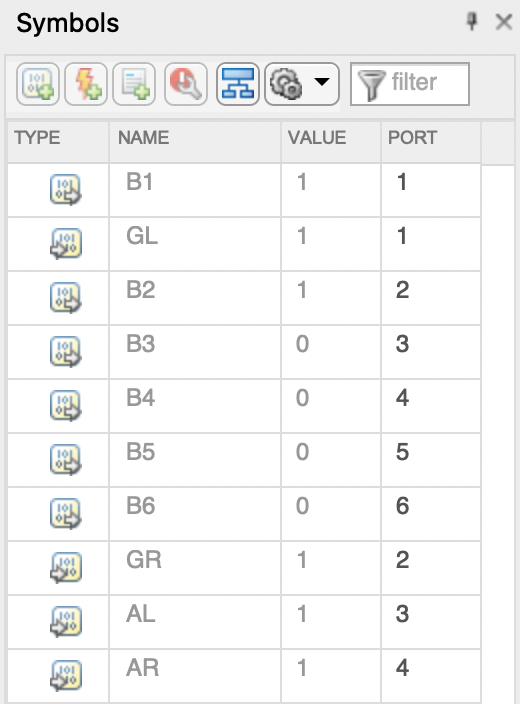
\includegraphics[width=4.25cm]{all_powered_signals.png}
\end{center}
\begin{center}
\small{Figure 2.2.4 BPCU Output Control Signals}
\end{center}
\begin{center}
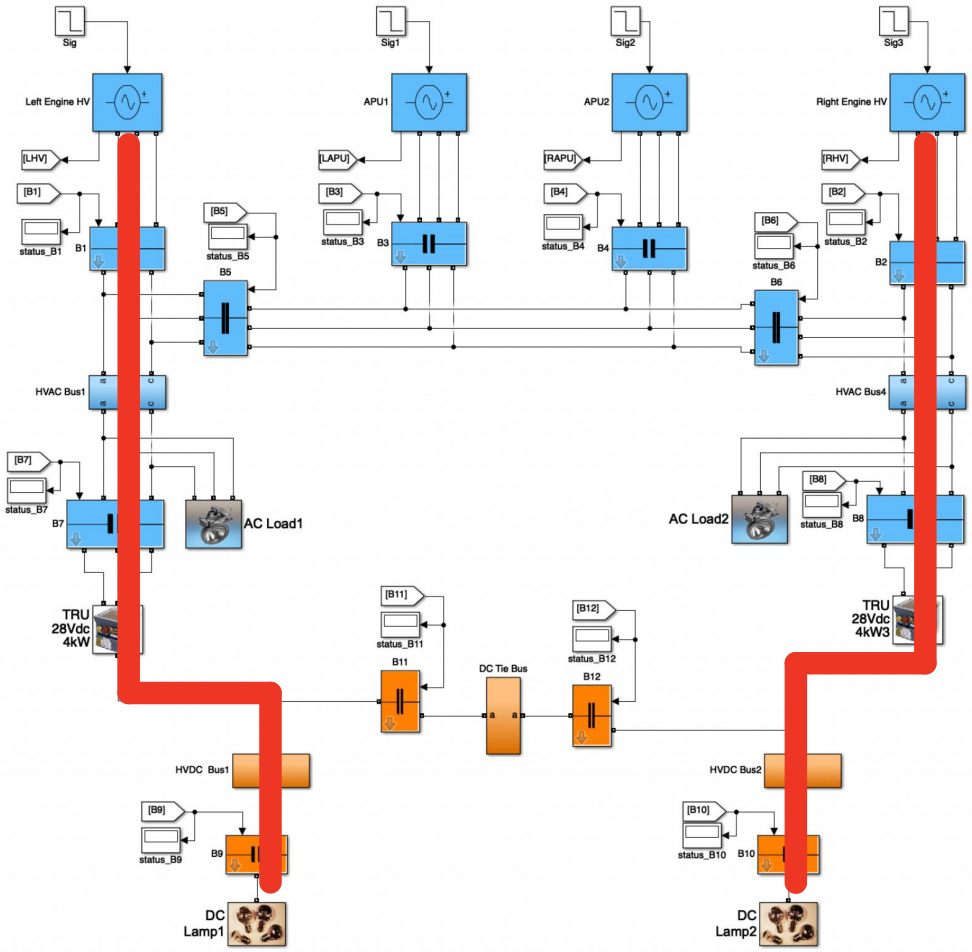
\includegraphics[width=13.5cm]{all_powered.png}
\end{center}
\begin{center}
\small{Figure 2.2.5 EPS Connection}
\end{center}
Under normal conditions, GL empowers the left AC bus, GR empowers the right AC bus. 
\pagebreak

\subsection{Case 2: GR Not Working}
\settowidth{\imageheight}{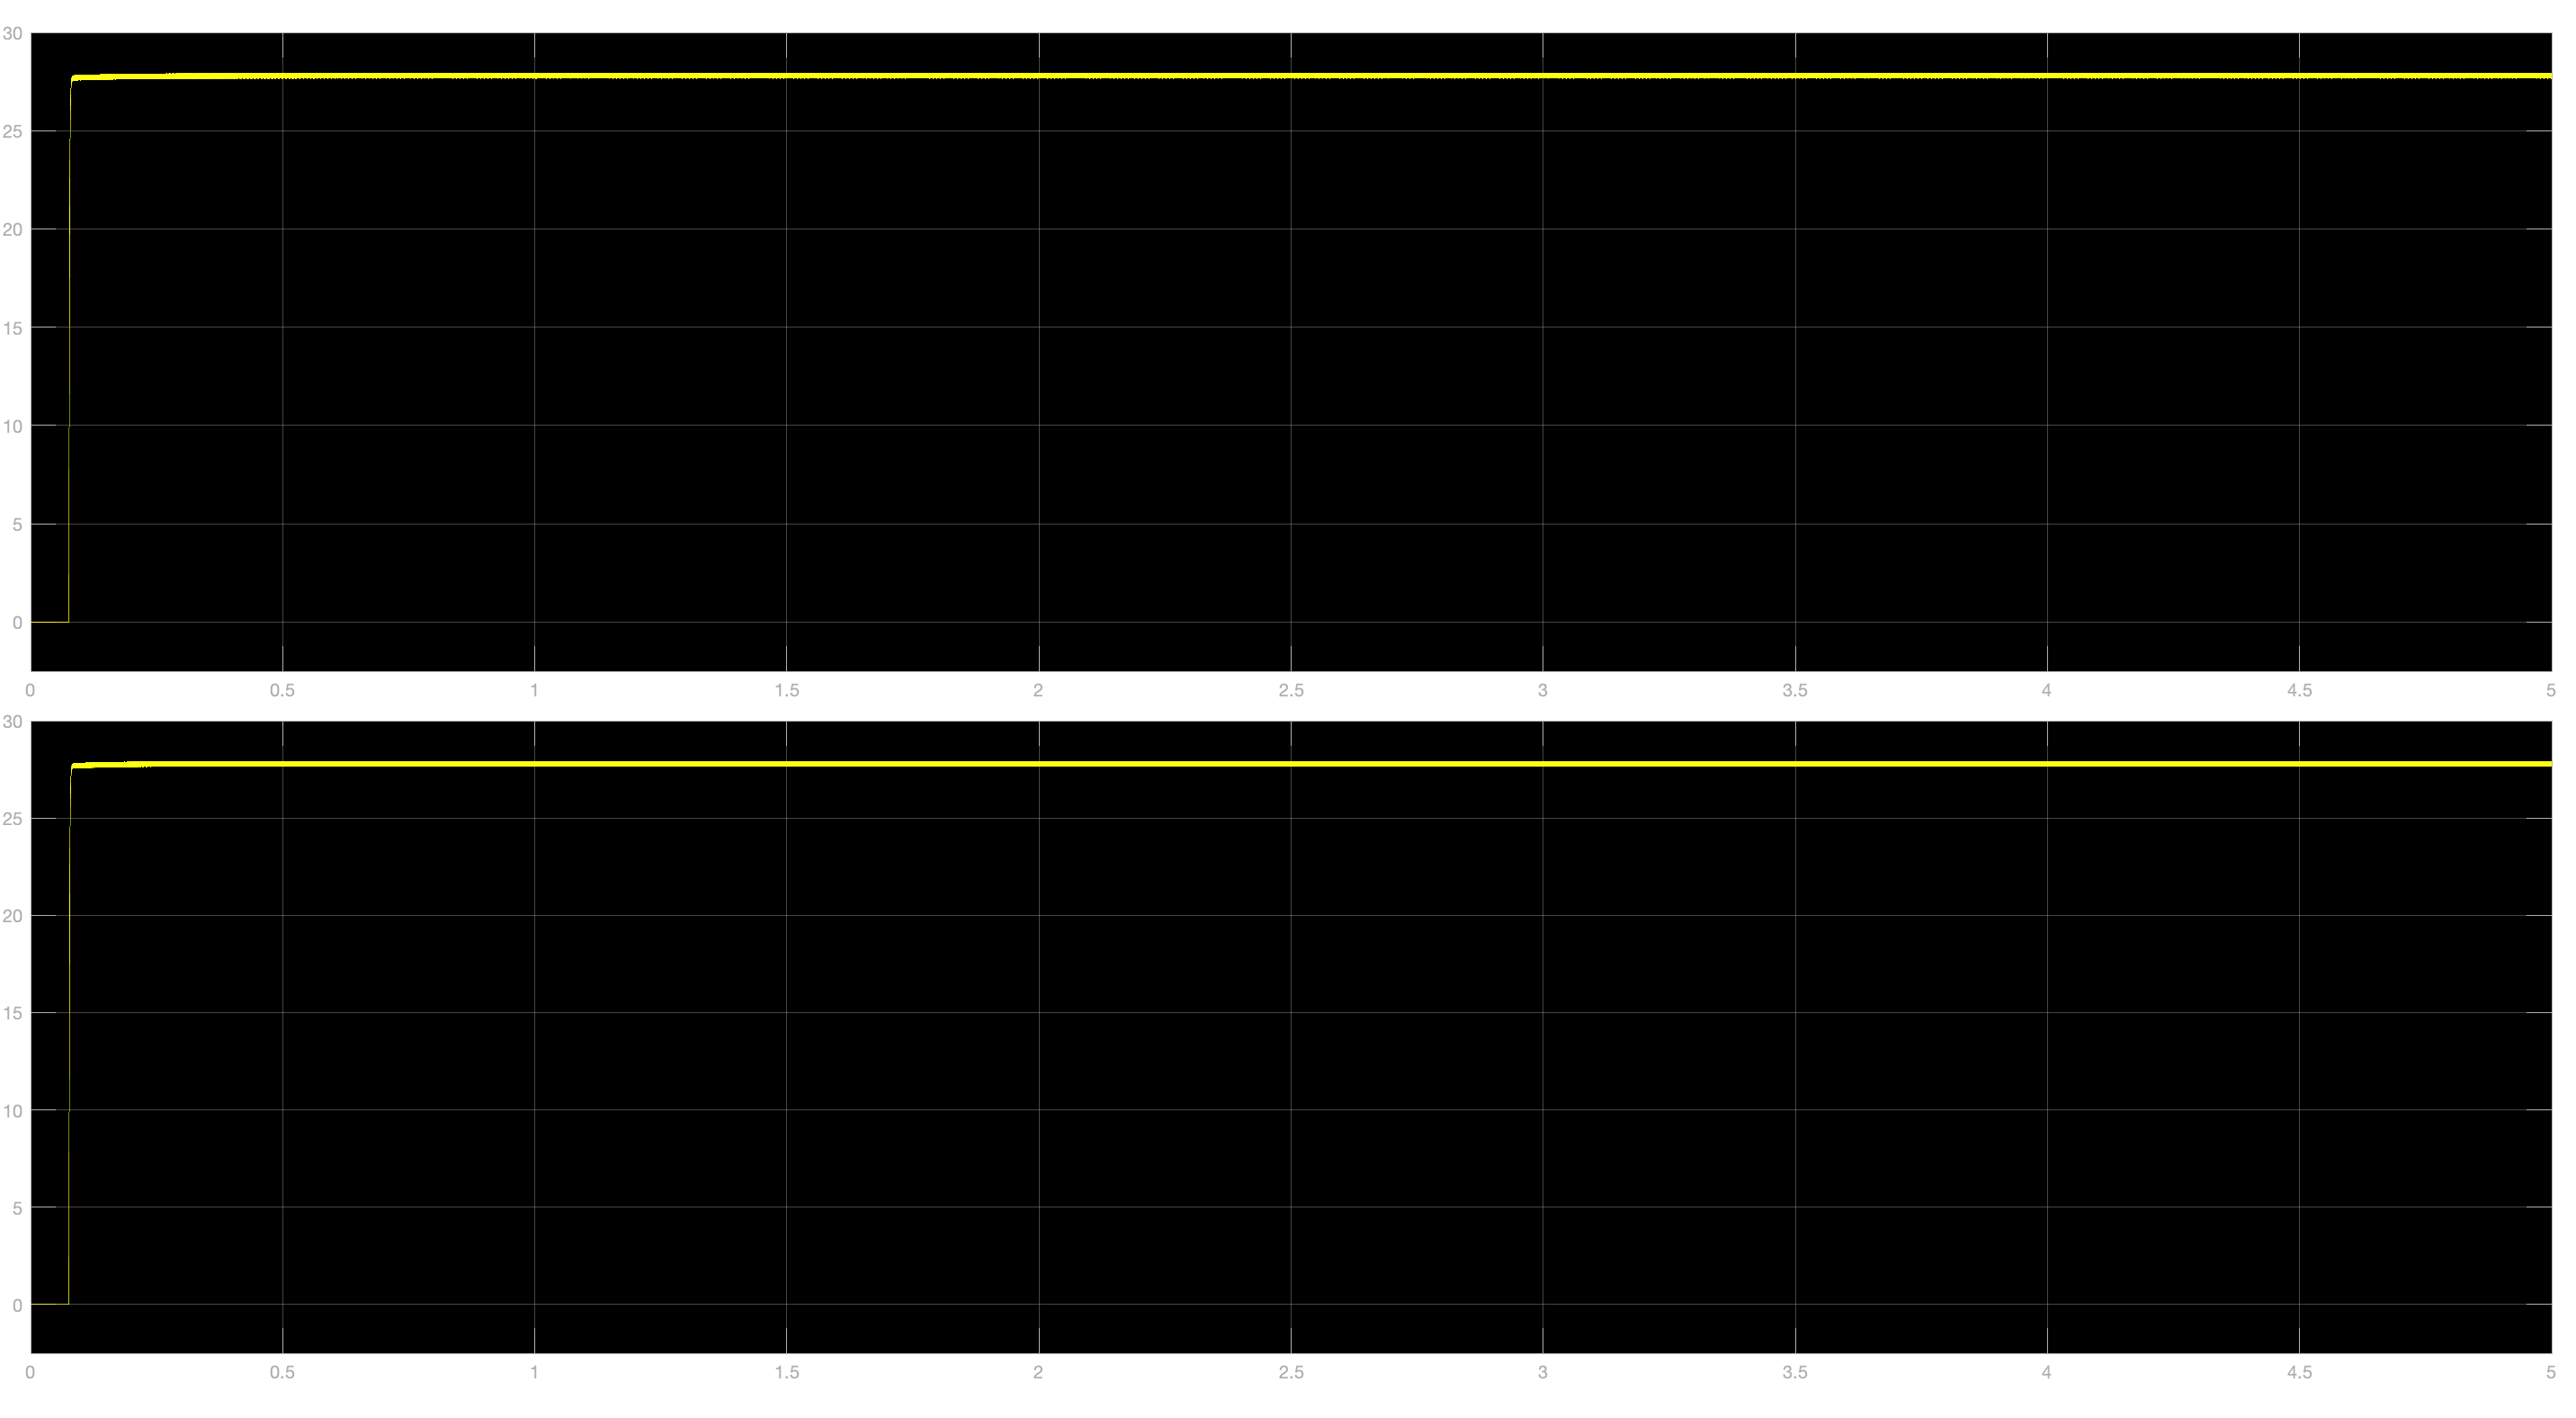
\includegraphics{gr_down_load1.png}}
\begin{center}
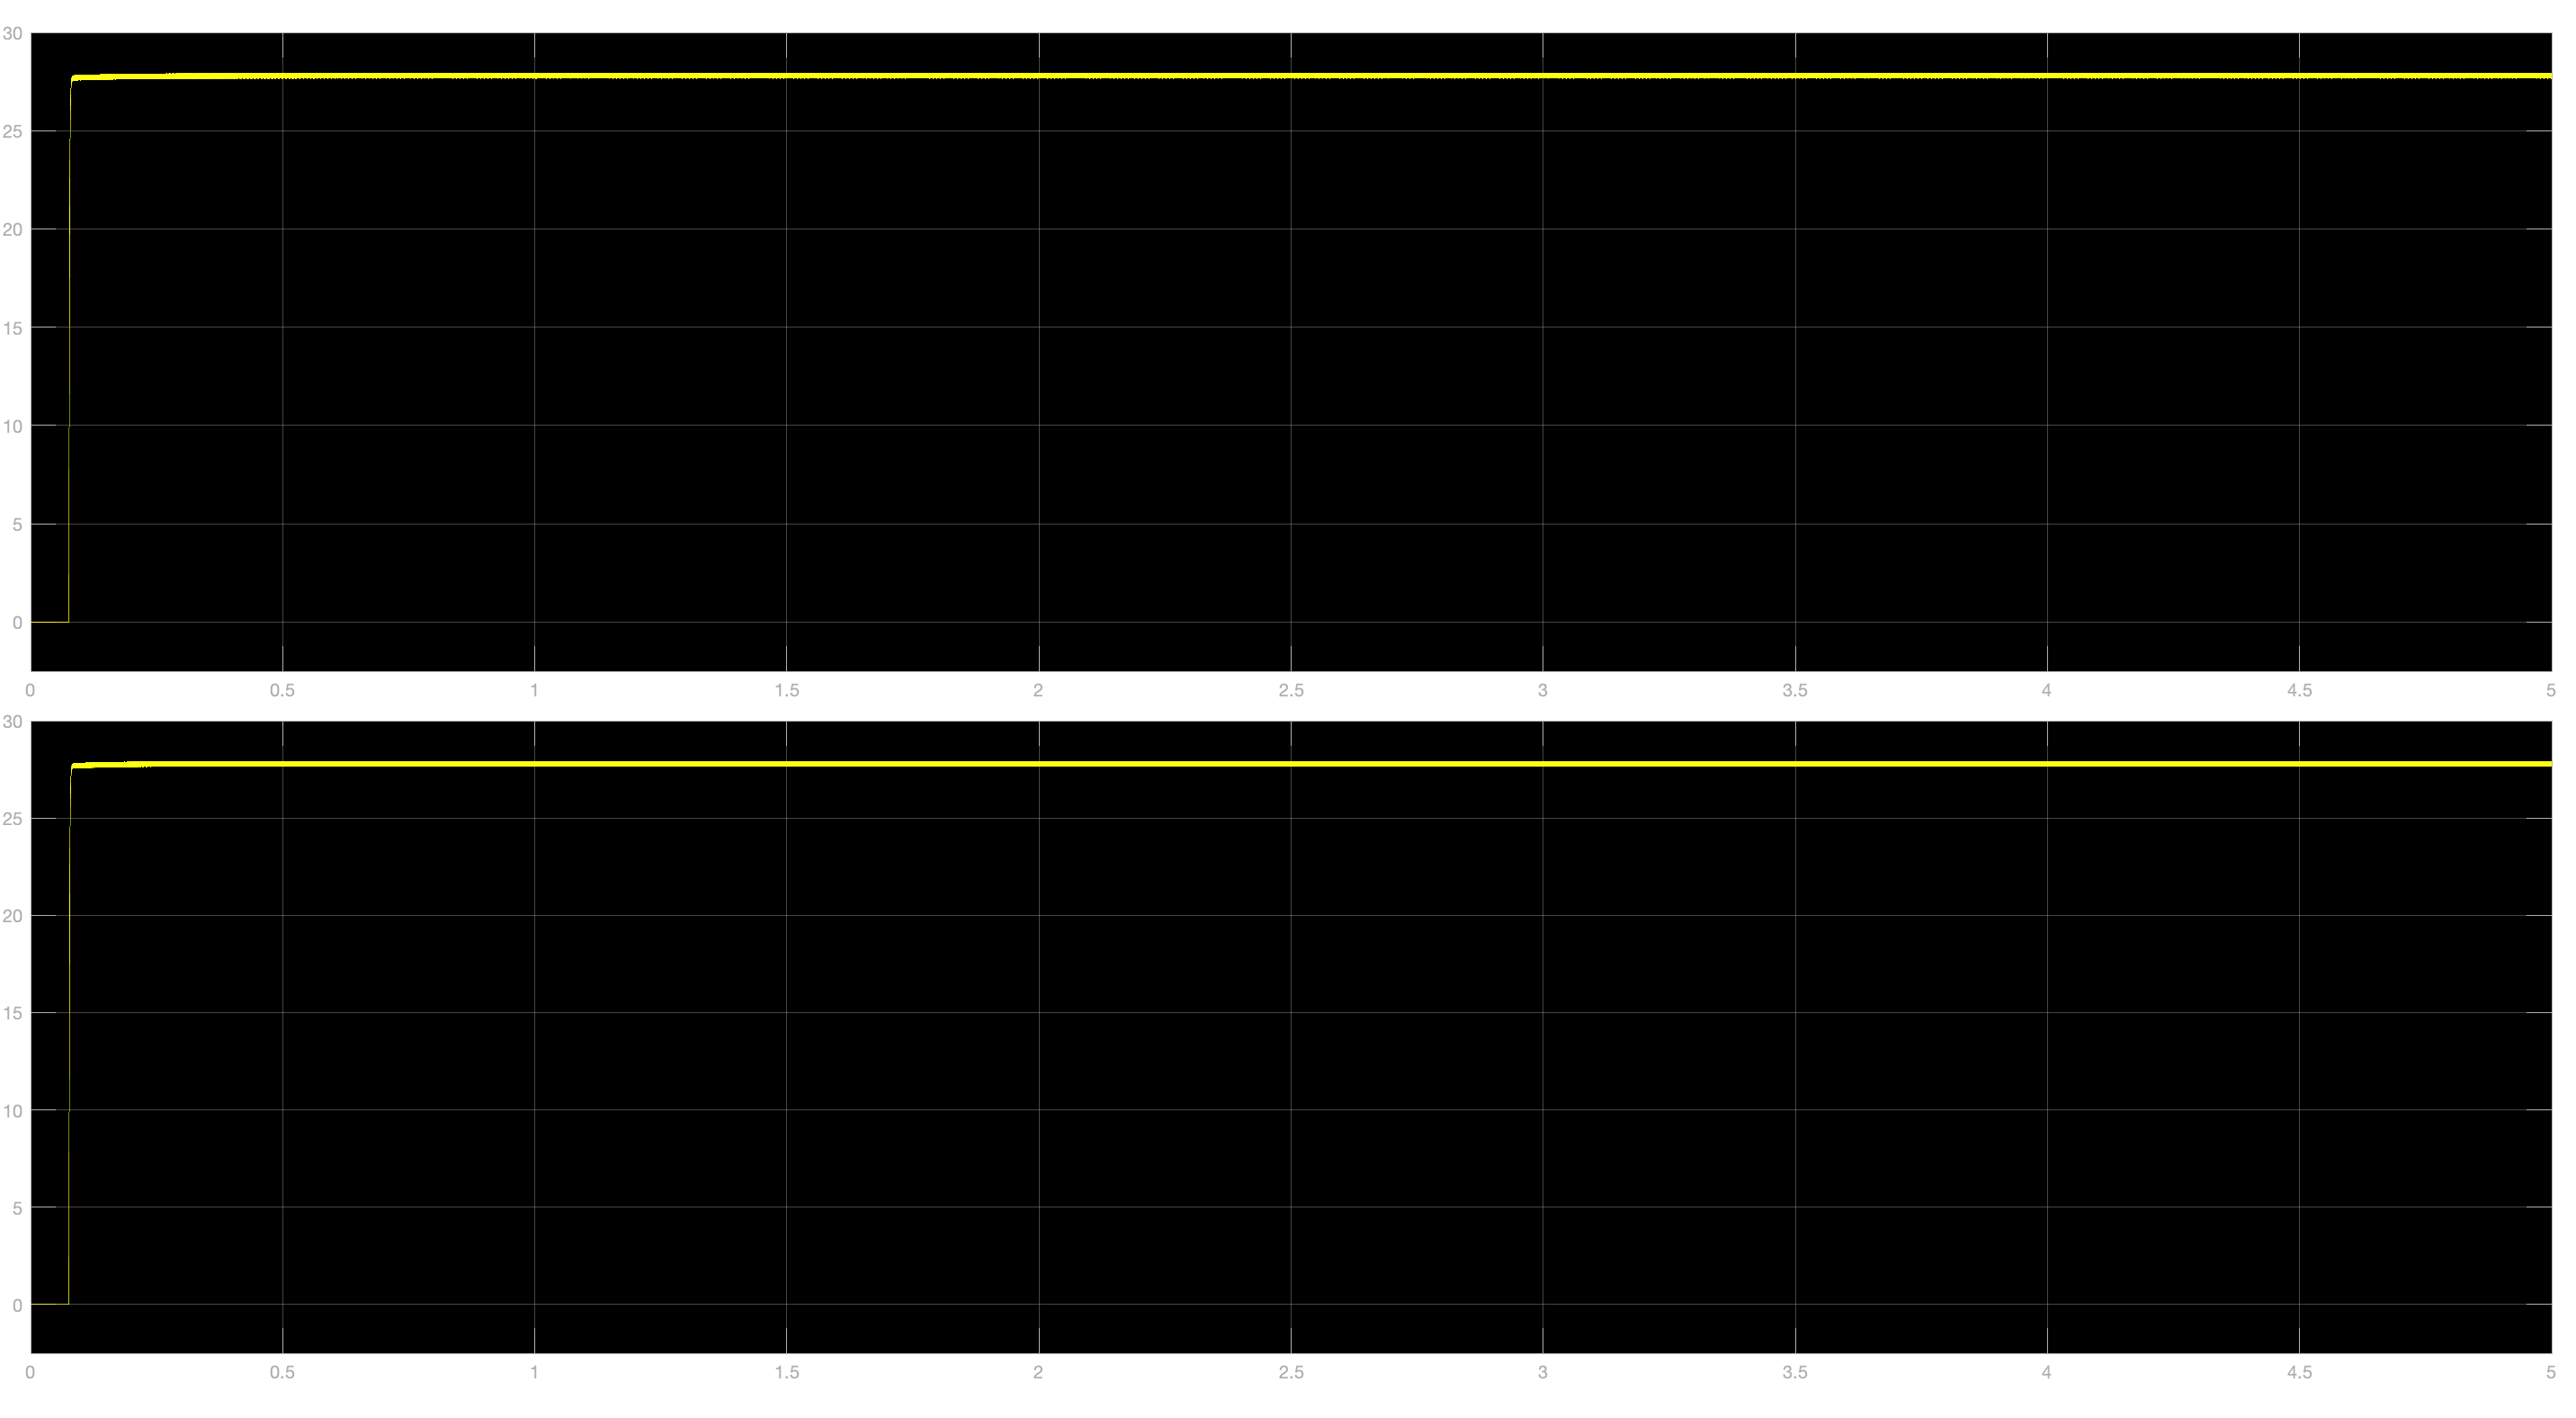
\includegraphics[trim= 0 0.28\imageheight{} 0 0, clip, width = 0.165\imageheight{}]{gr_down_load1.png}
\end{center}
\begin{center}
\small{Figure 2.3.1 Left DC Load Waveform}
\end{center}
\settowidth{\imageheight}{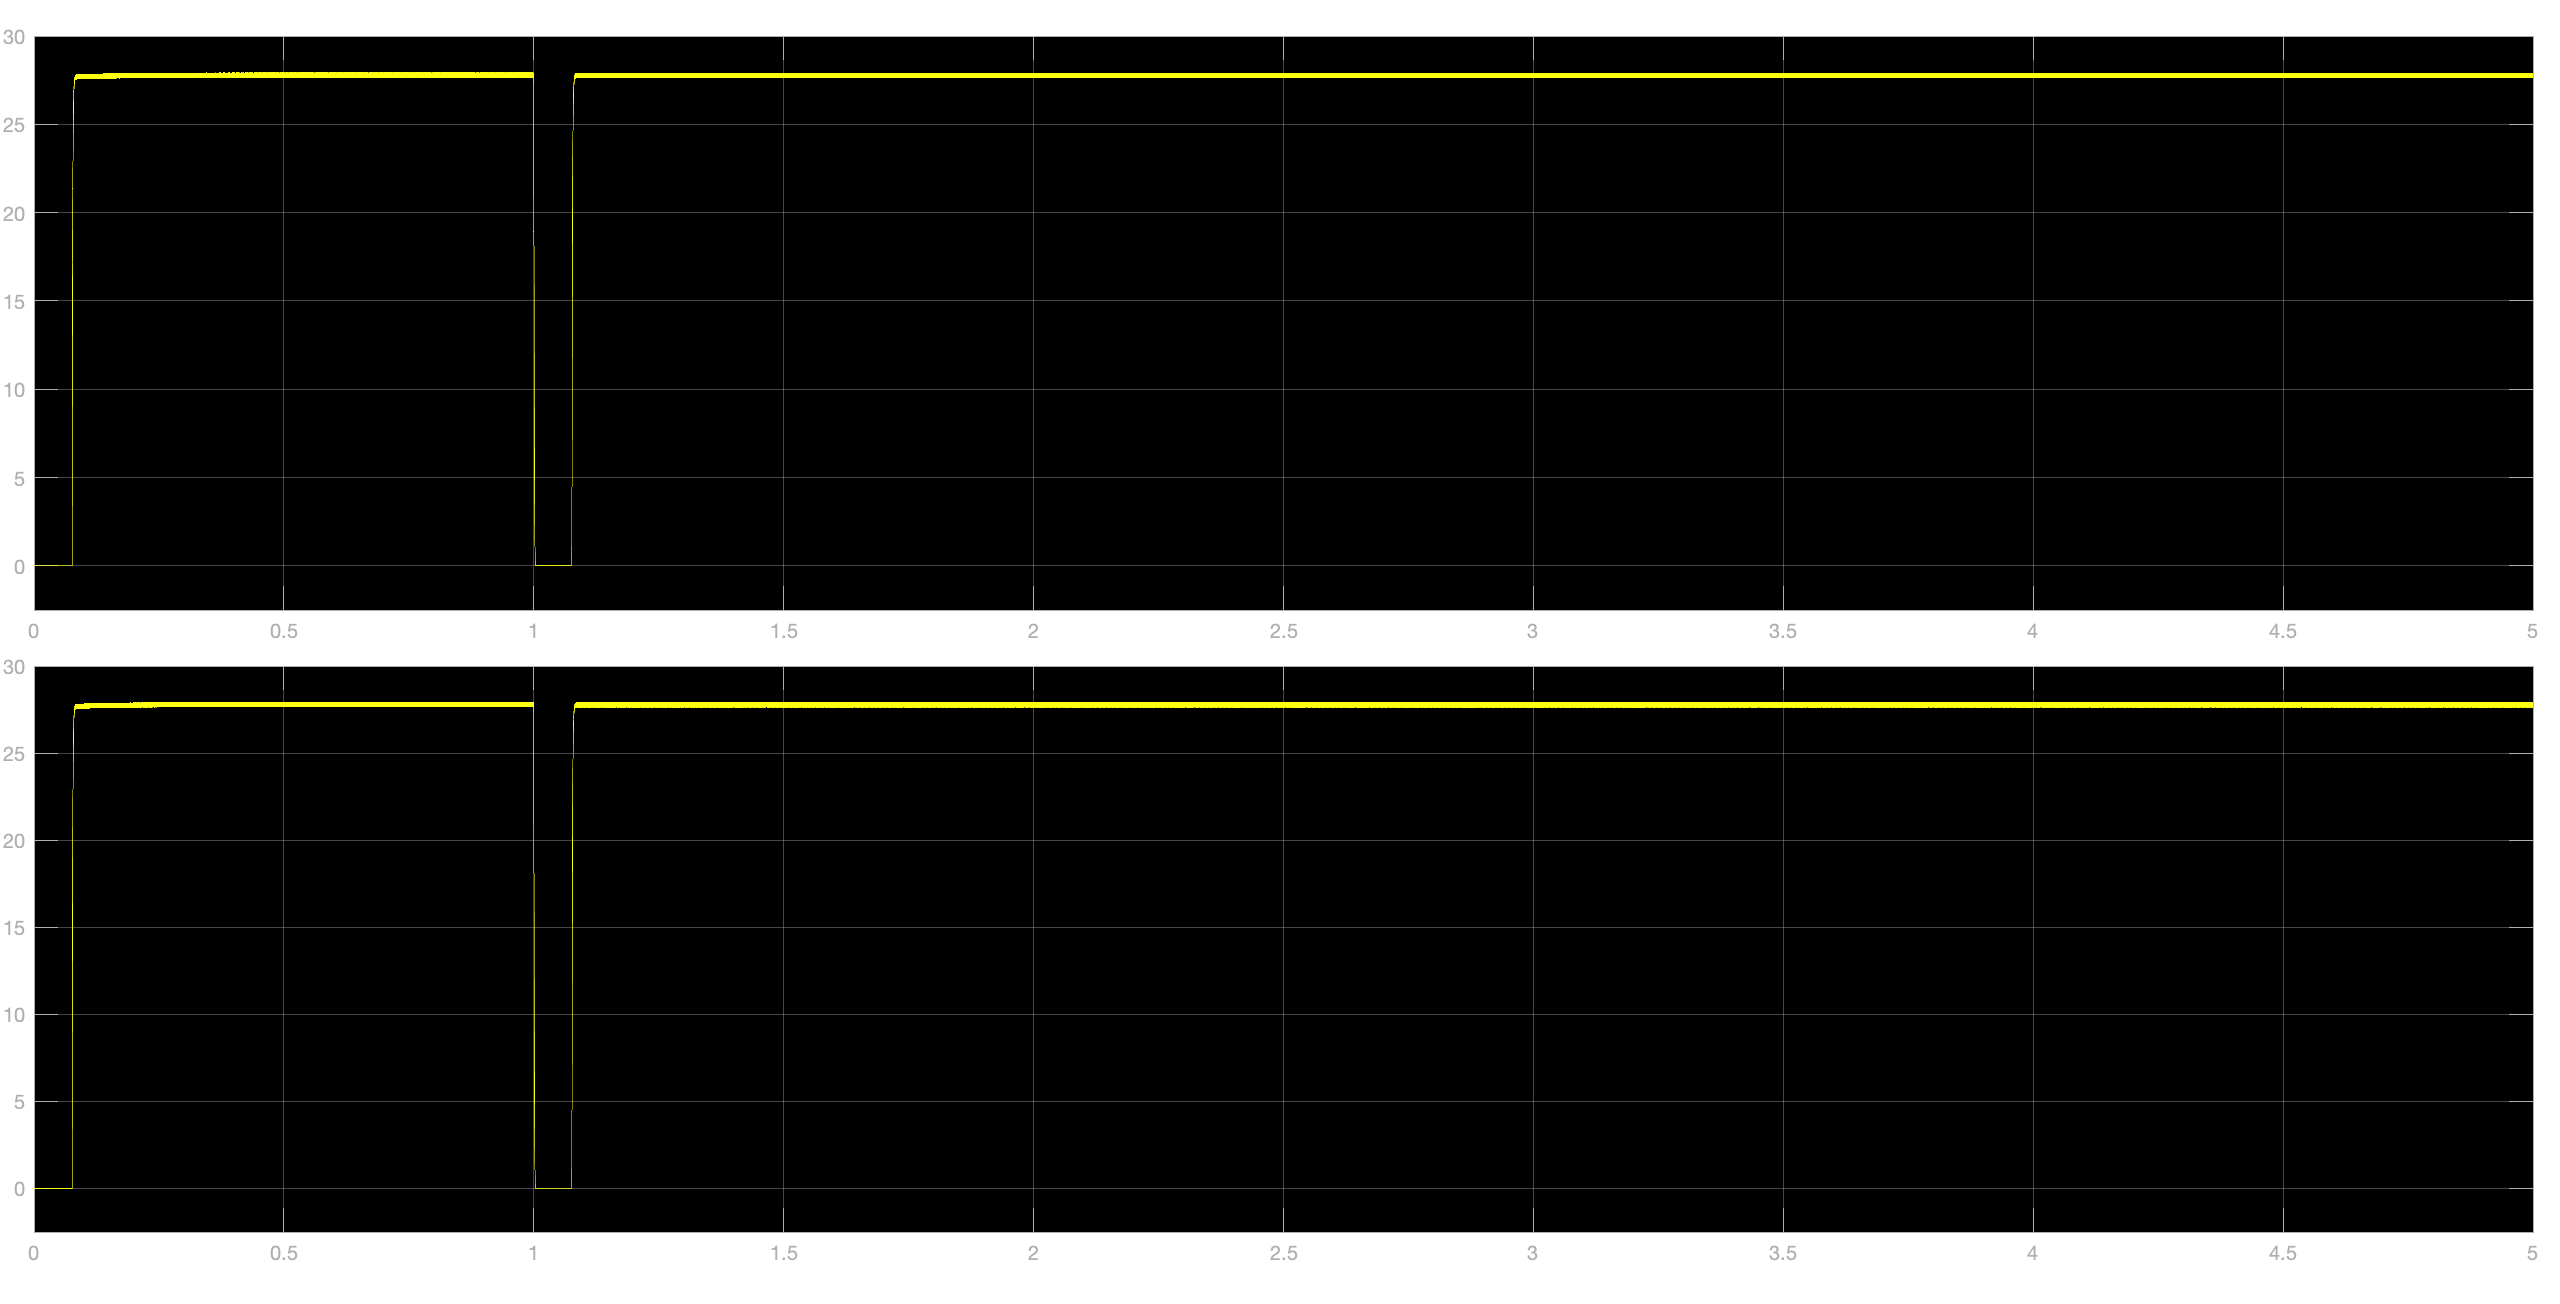
\includegraphics{gr_down_load2.png}}
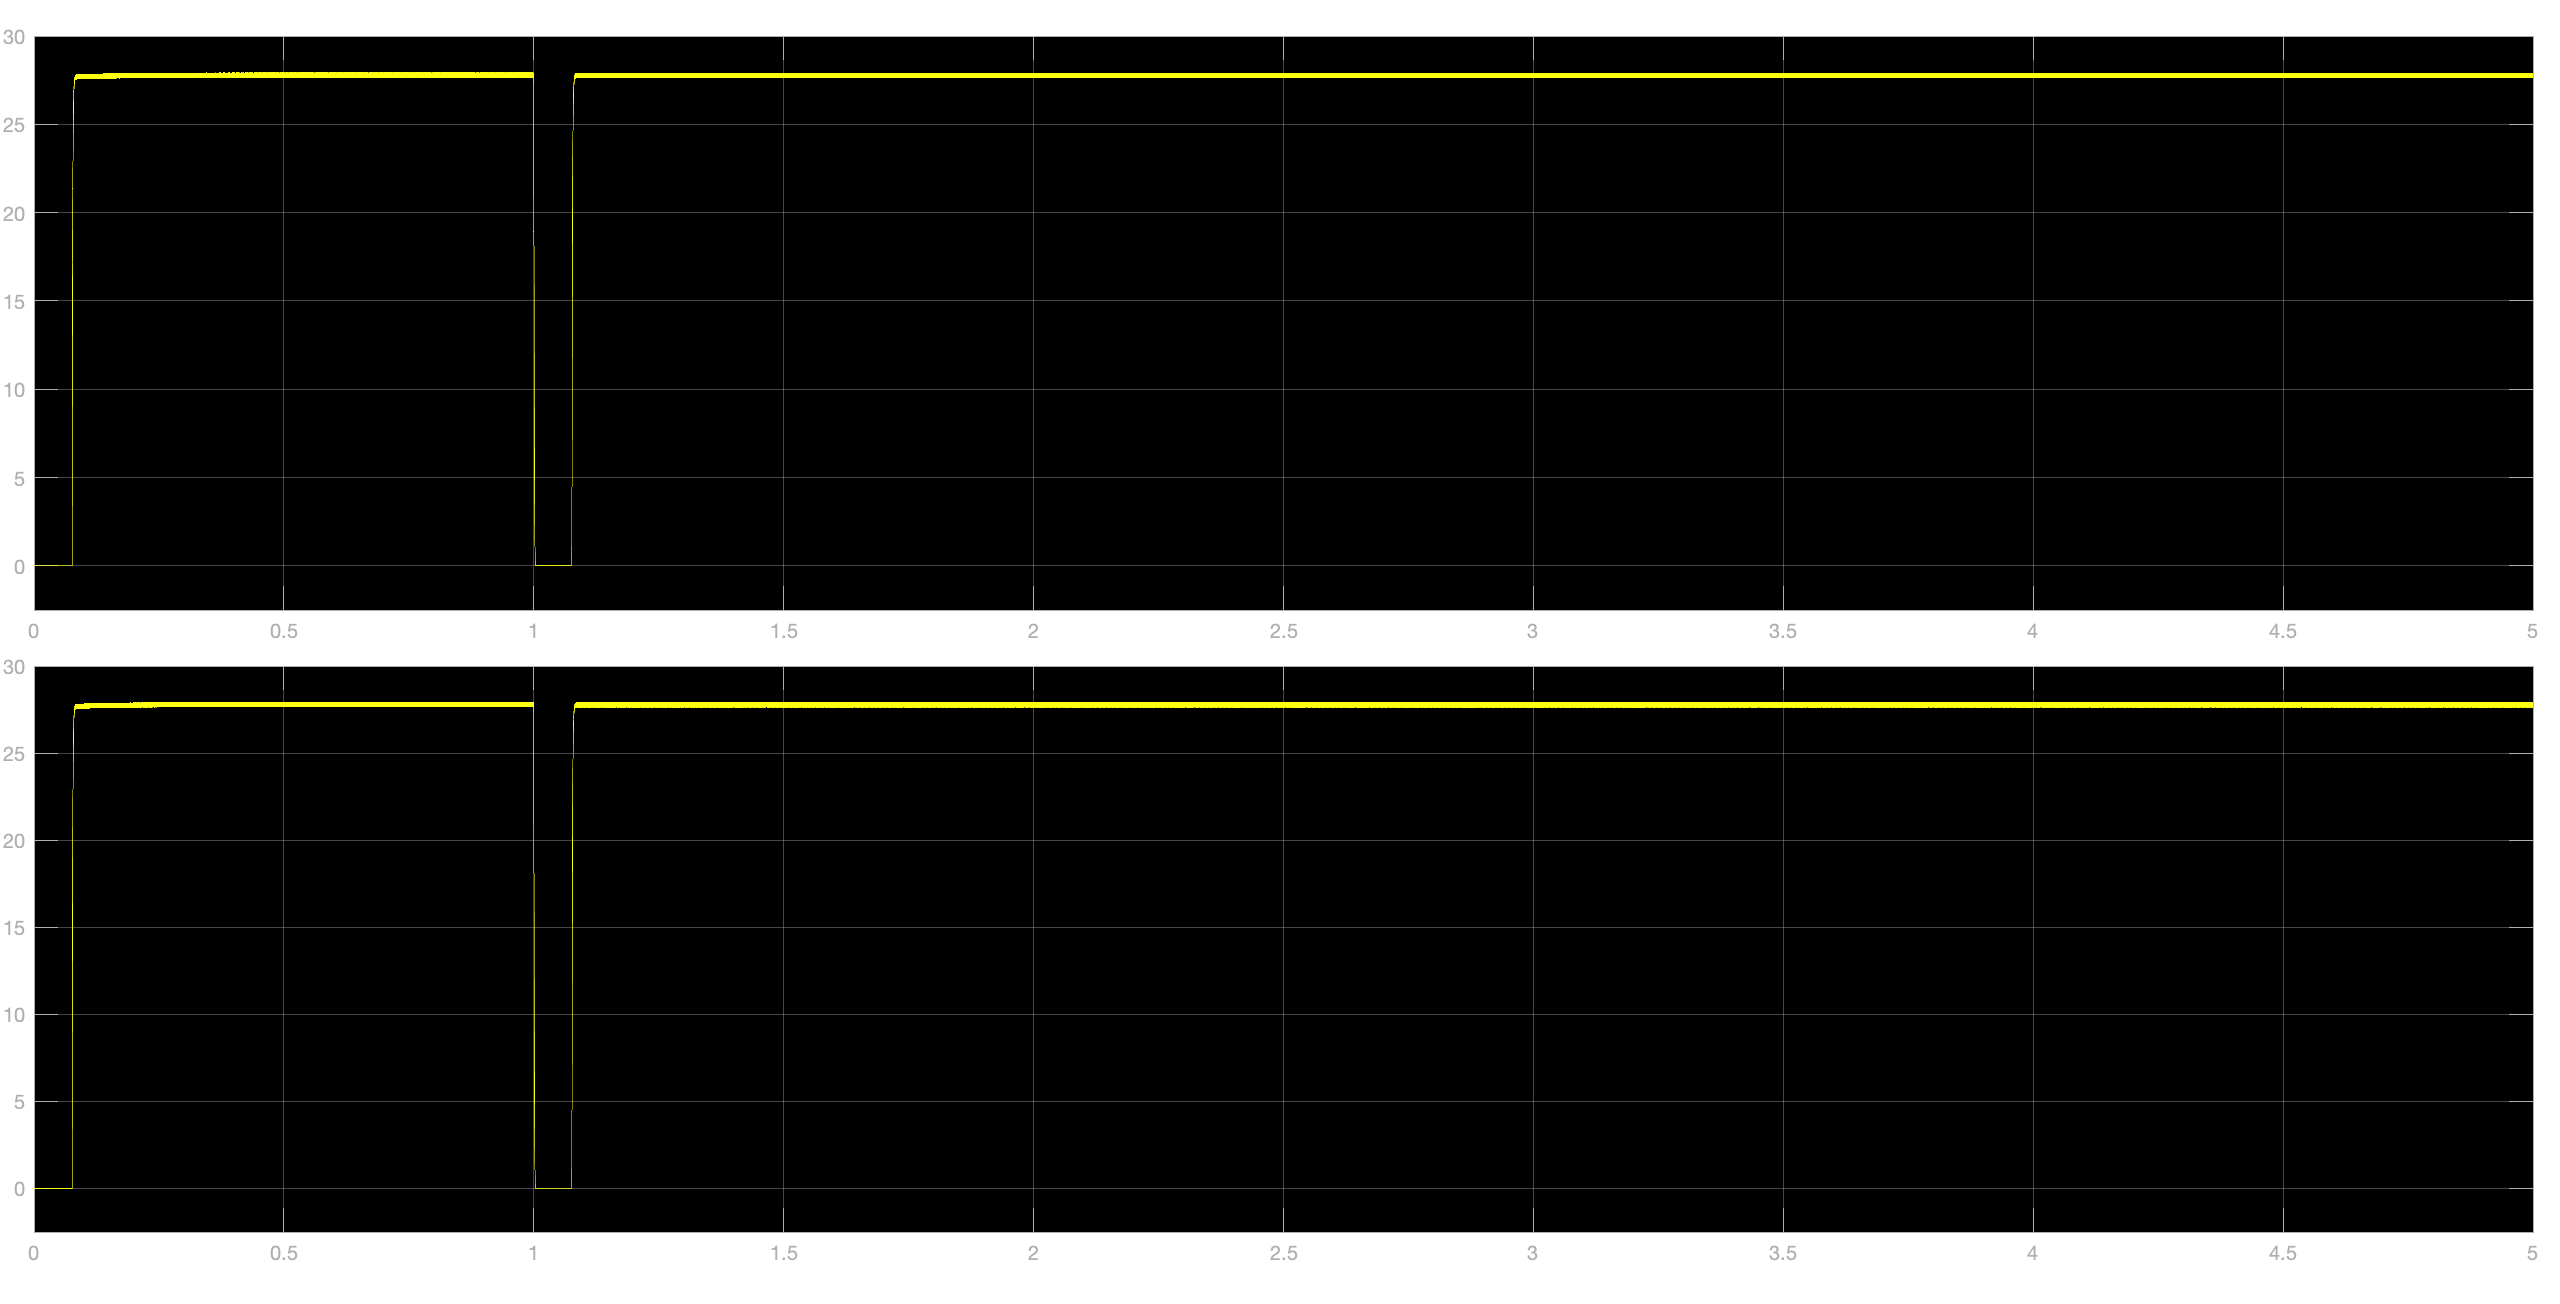
\includegraphics[trim= 0 0.255\imageheight{} 0 0, clip, width = 0.185\imageheight{}]{gr_down_load2.png}
\begin{center}
\small{Figure 2.3.2 Right DC Load Waveform}
\end{center}
\begin{center}
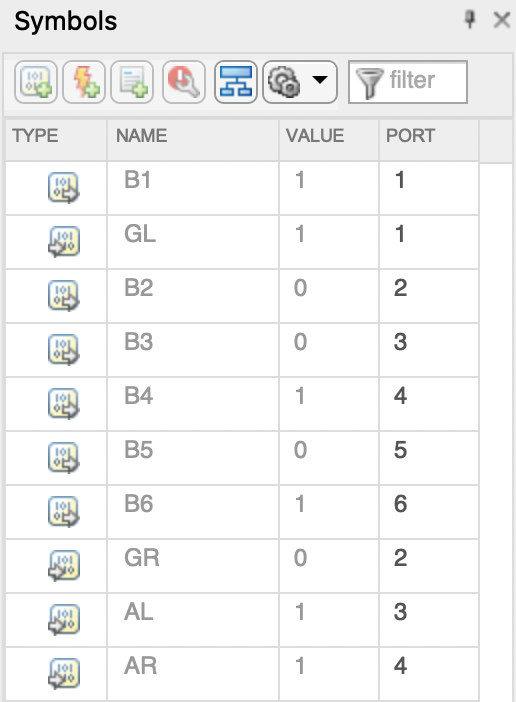
\includegraphics[width=4.5cm]{gr_down_signals.png}
\end{center}
\begin{center}
\small{Figure 2.3.3 BPCU Output Control Signals}
\end{center}
\begin{center}
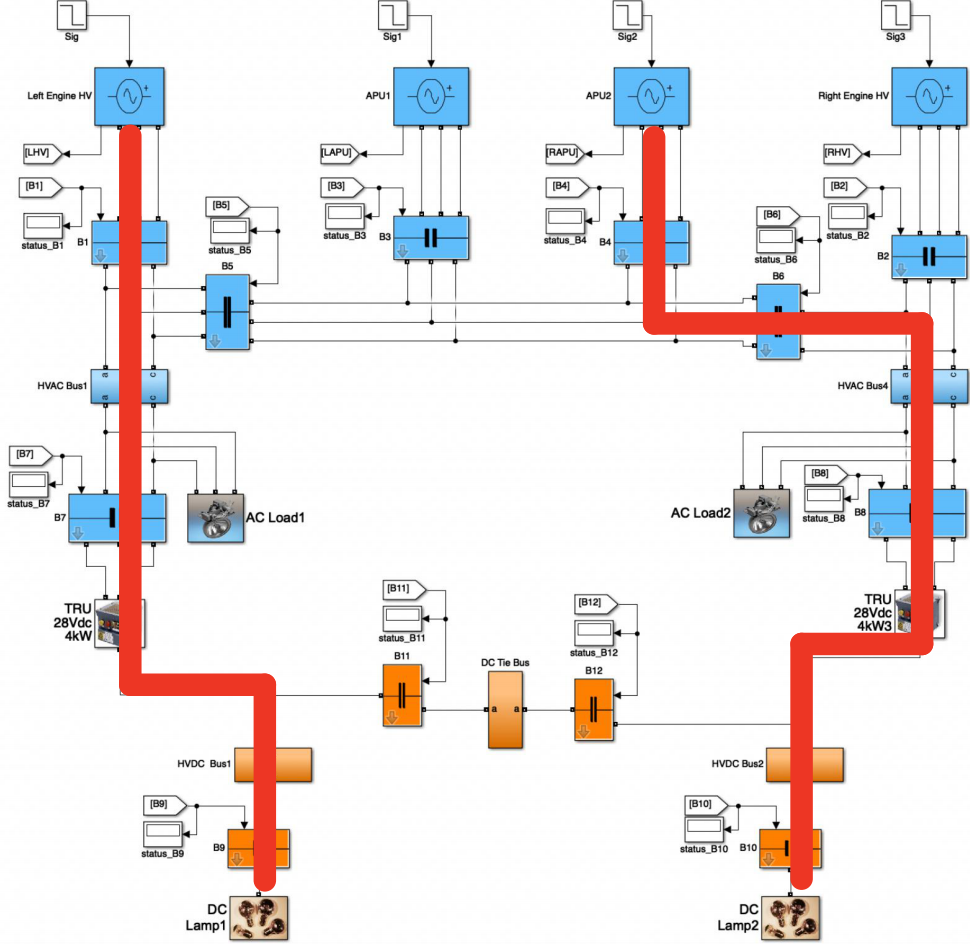
\includegraphics[width=14.5cm]{gr_down.png}
\end{center}
\begin{center}
\small{Figure 2.3.4 EPS Connection}
\end{center}
When only GR fails,  the rightmost available power supply AR empowers the right AC bus based on system guarantee G8. Only one APU, AR, is used based on system guarantee G4.
\pagebreak

\subsection{Case 3: GL Not Working}
\settowidth{\imageheight}{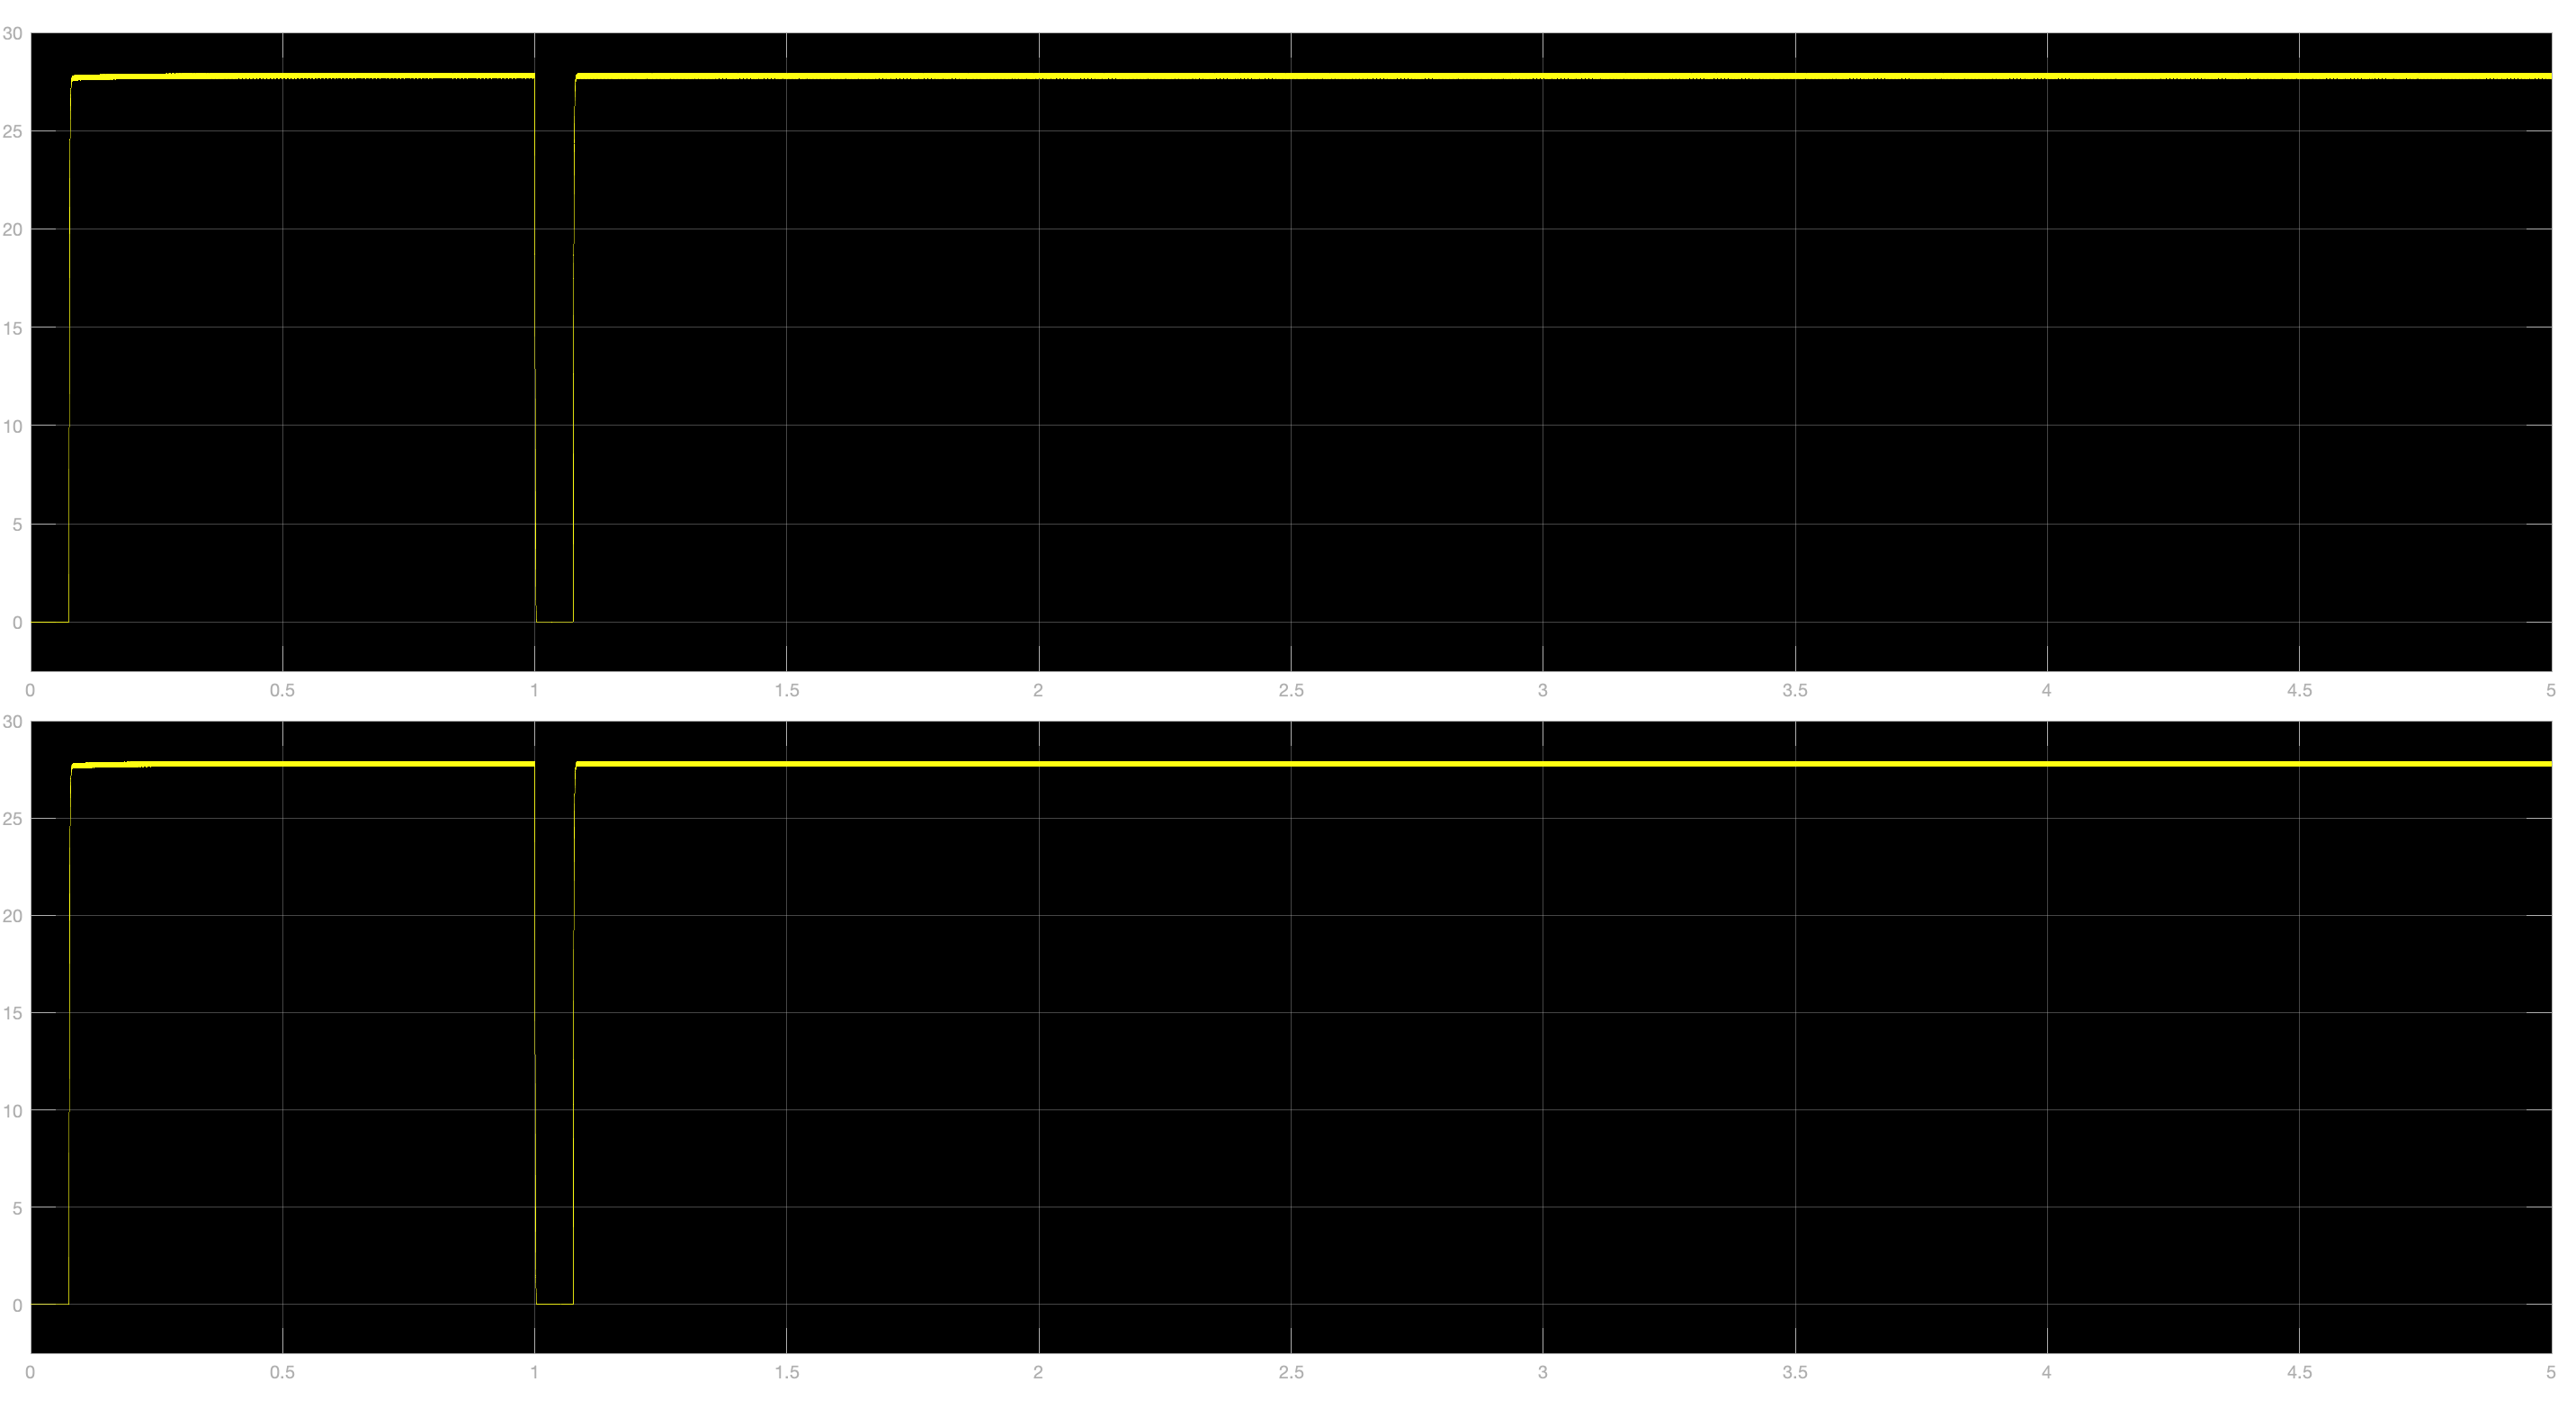
\includegraphics{gl_down_load1.png}}
\begin{center}
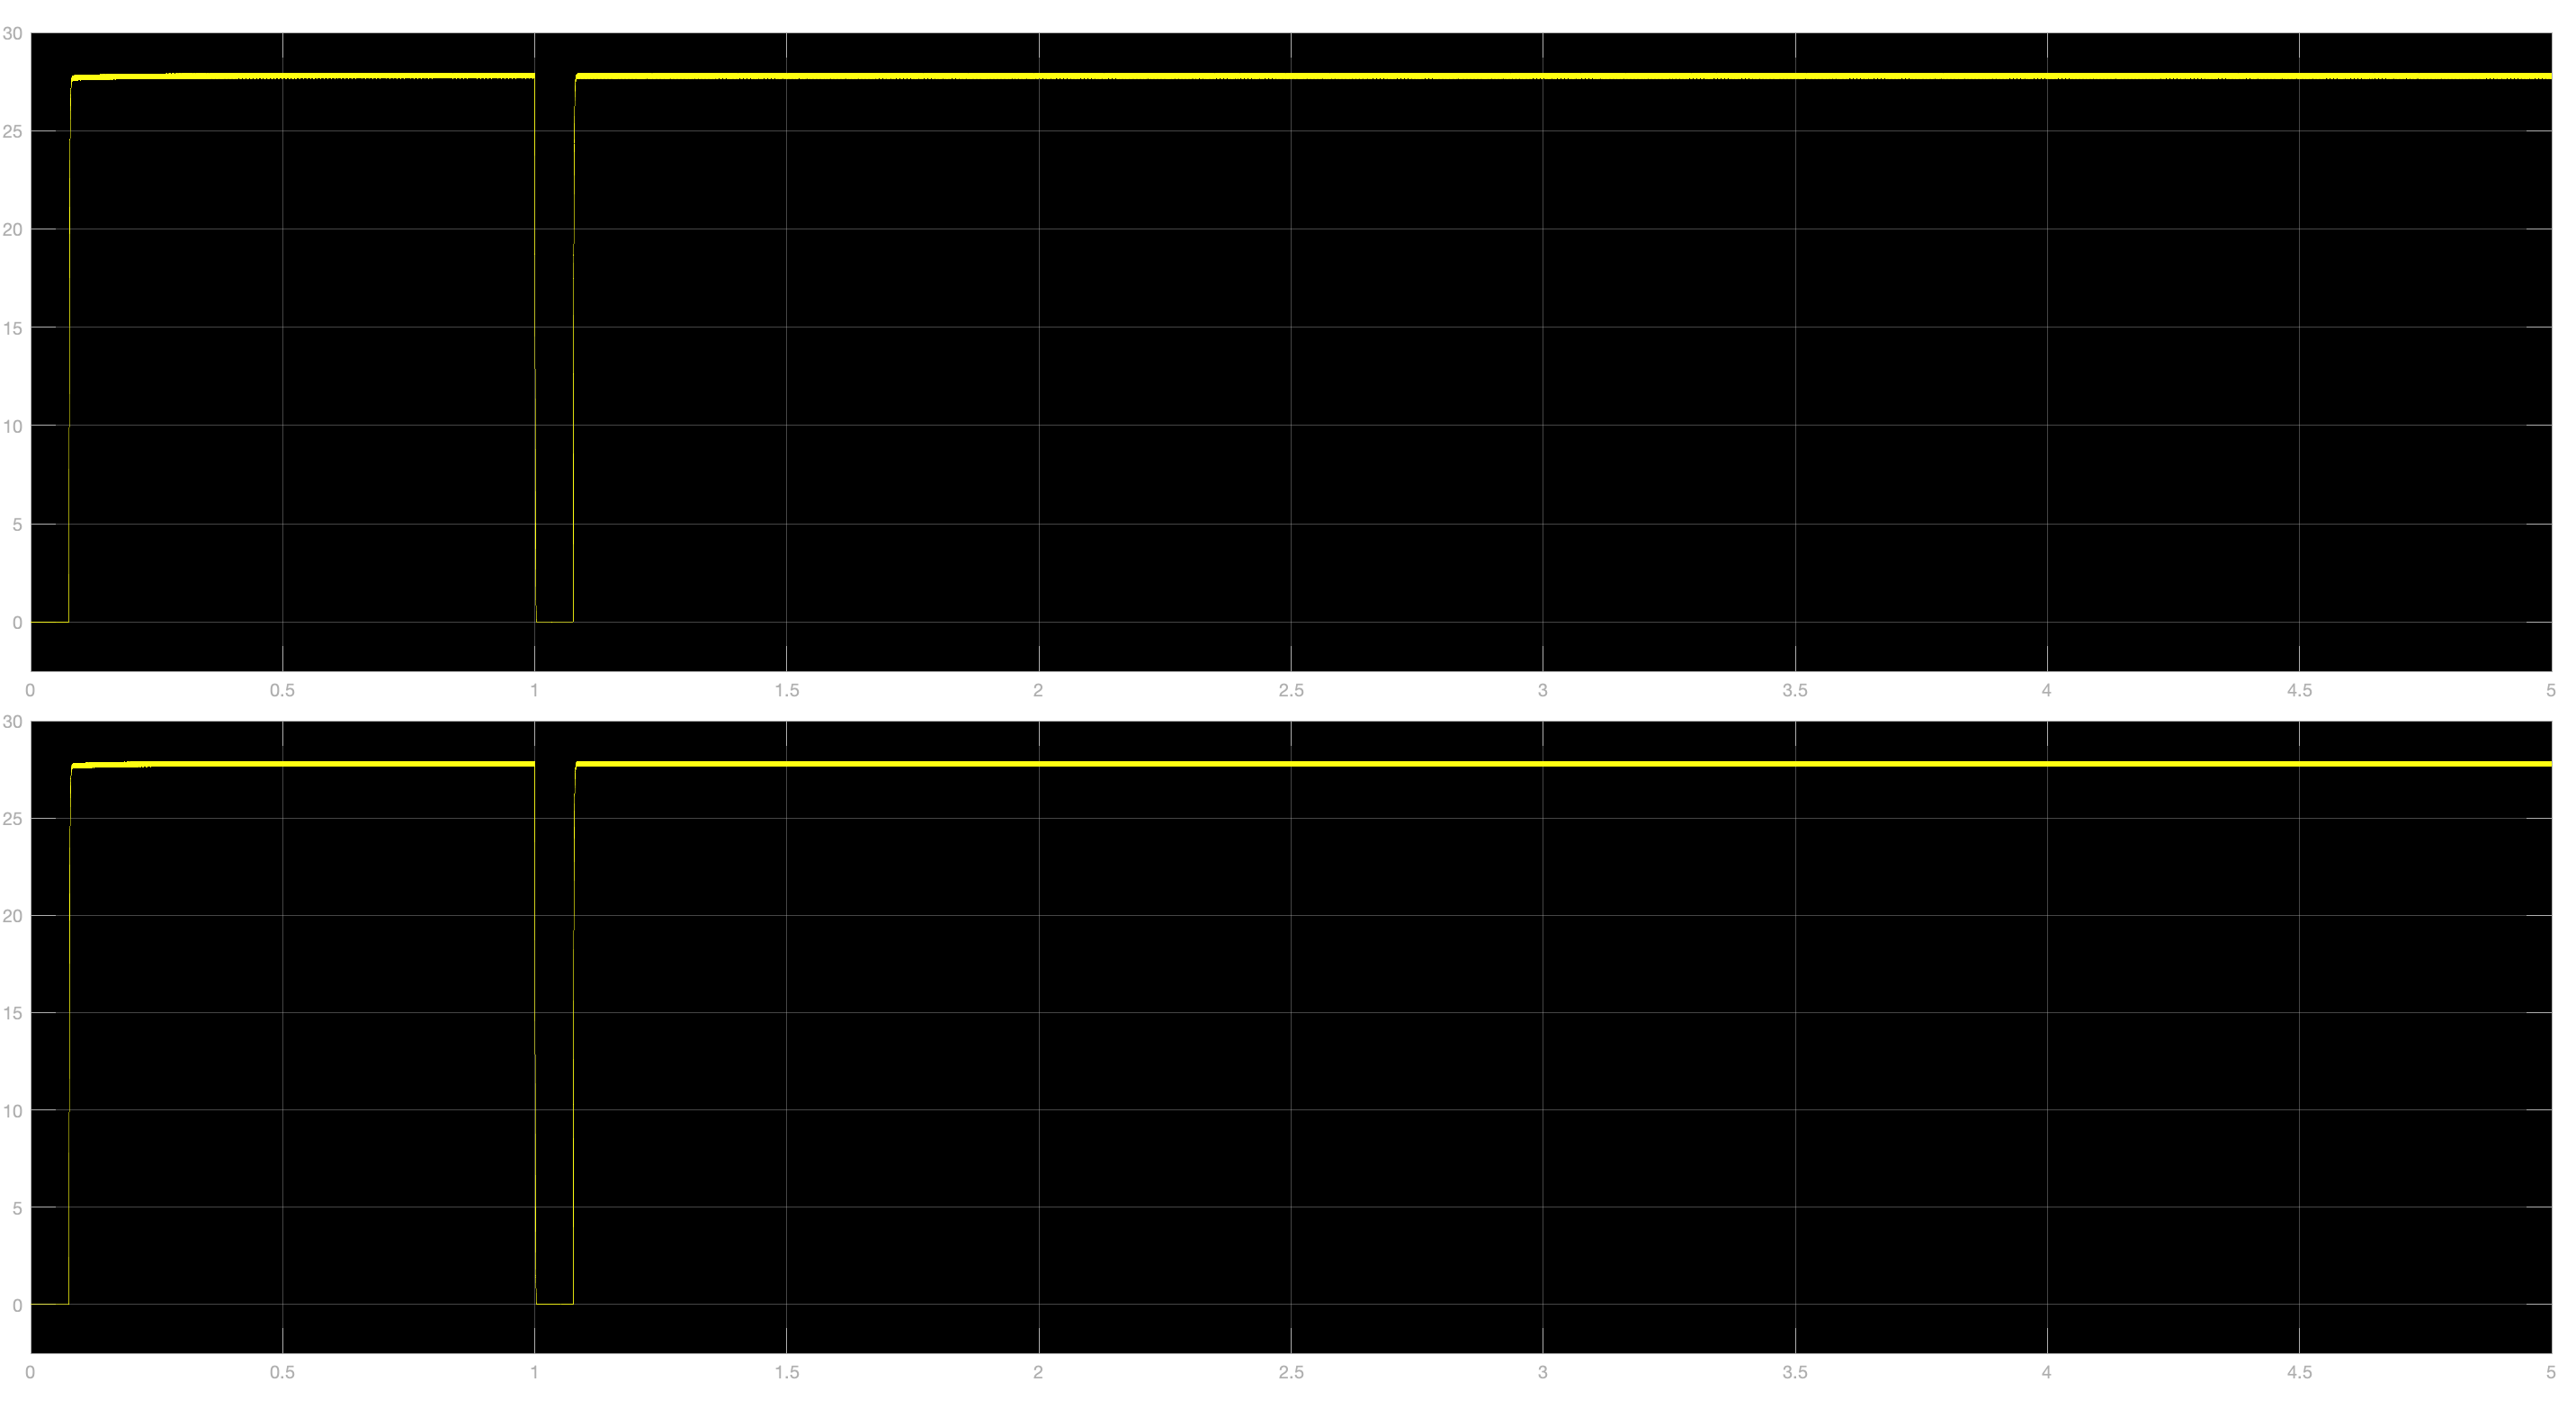
\includegraphics[trim= 0 0.28\imageheight{} 0 0, clip, width = 0.165\imageheight{}]{gl_down_load1.png}
\end{center}
\begin{center}
\small{Figure 2.4.1 Left DC Load Waveform}
\end{center}
\settowidth{\imageheight}{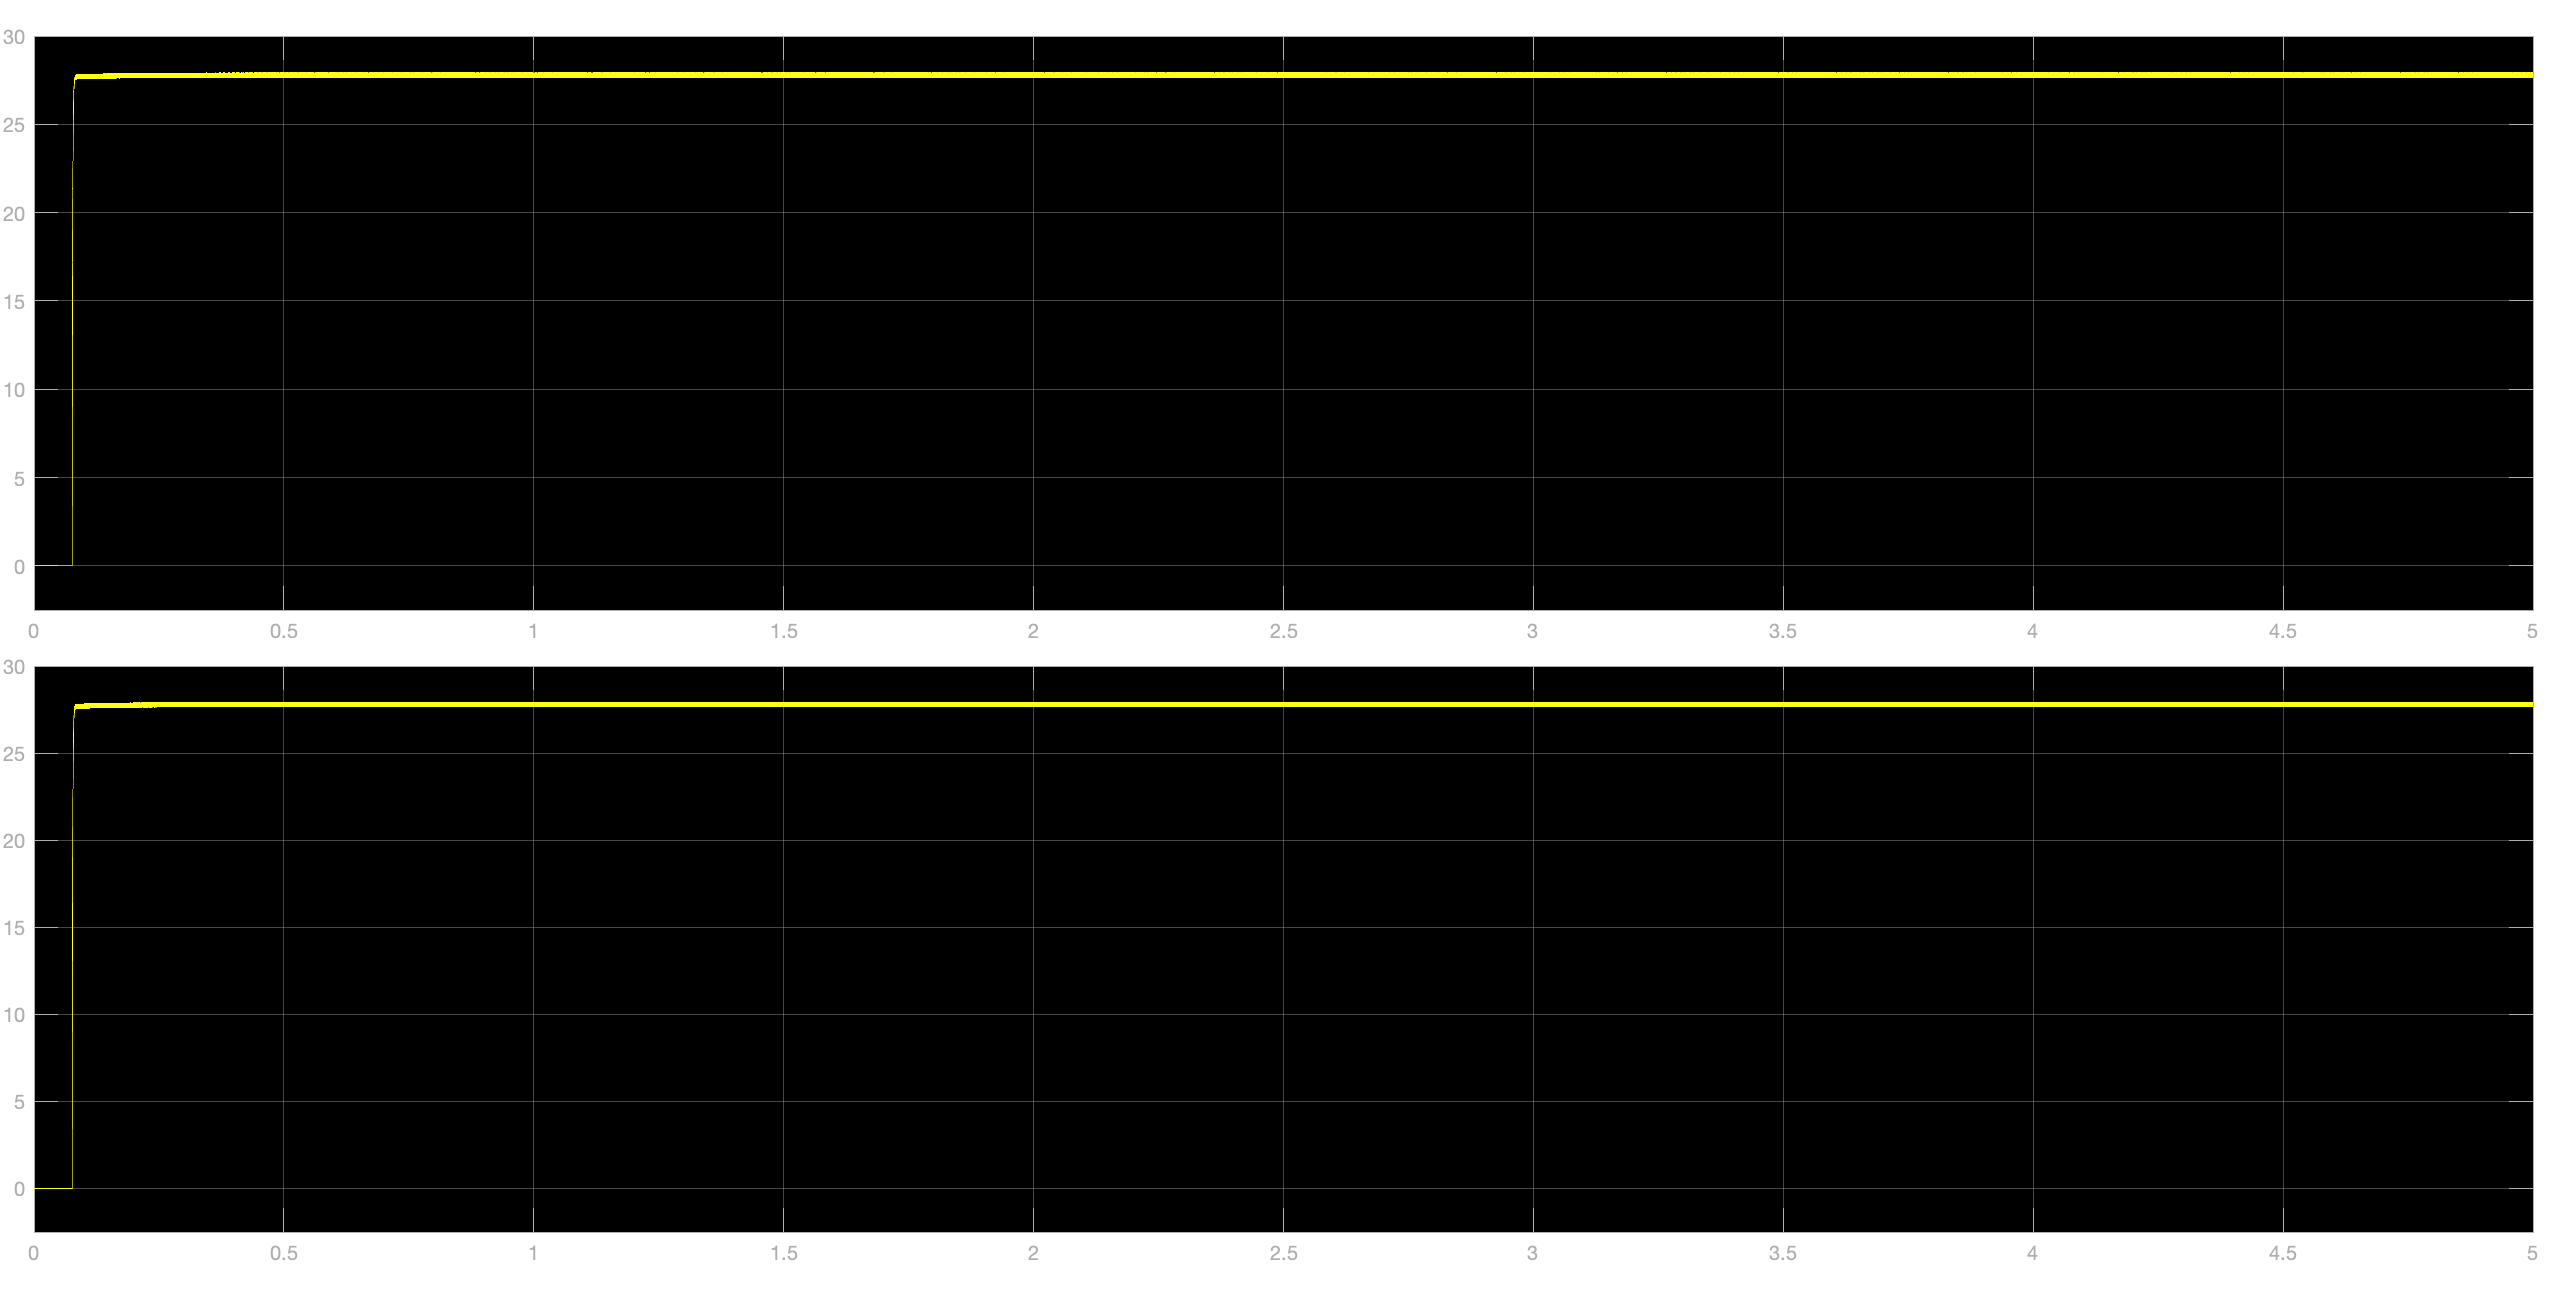
\includegraphics{gl_down_load2.png}}
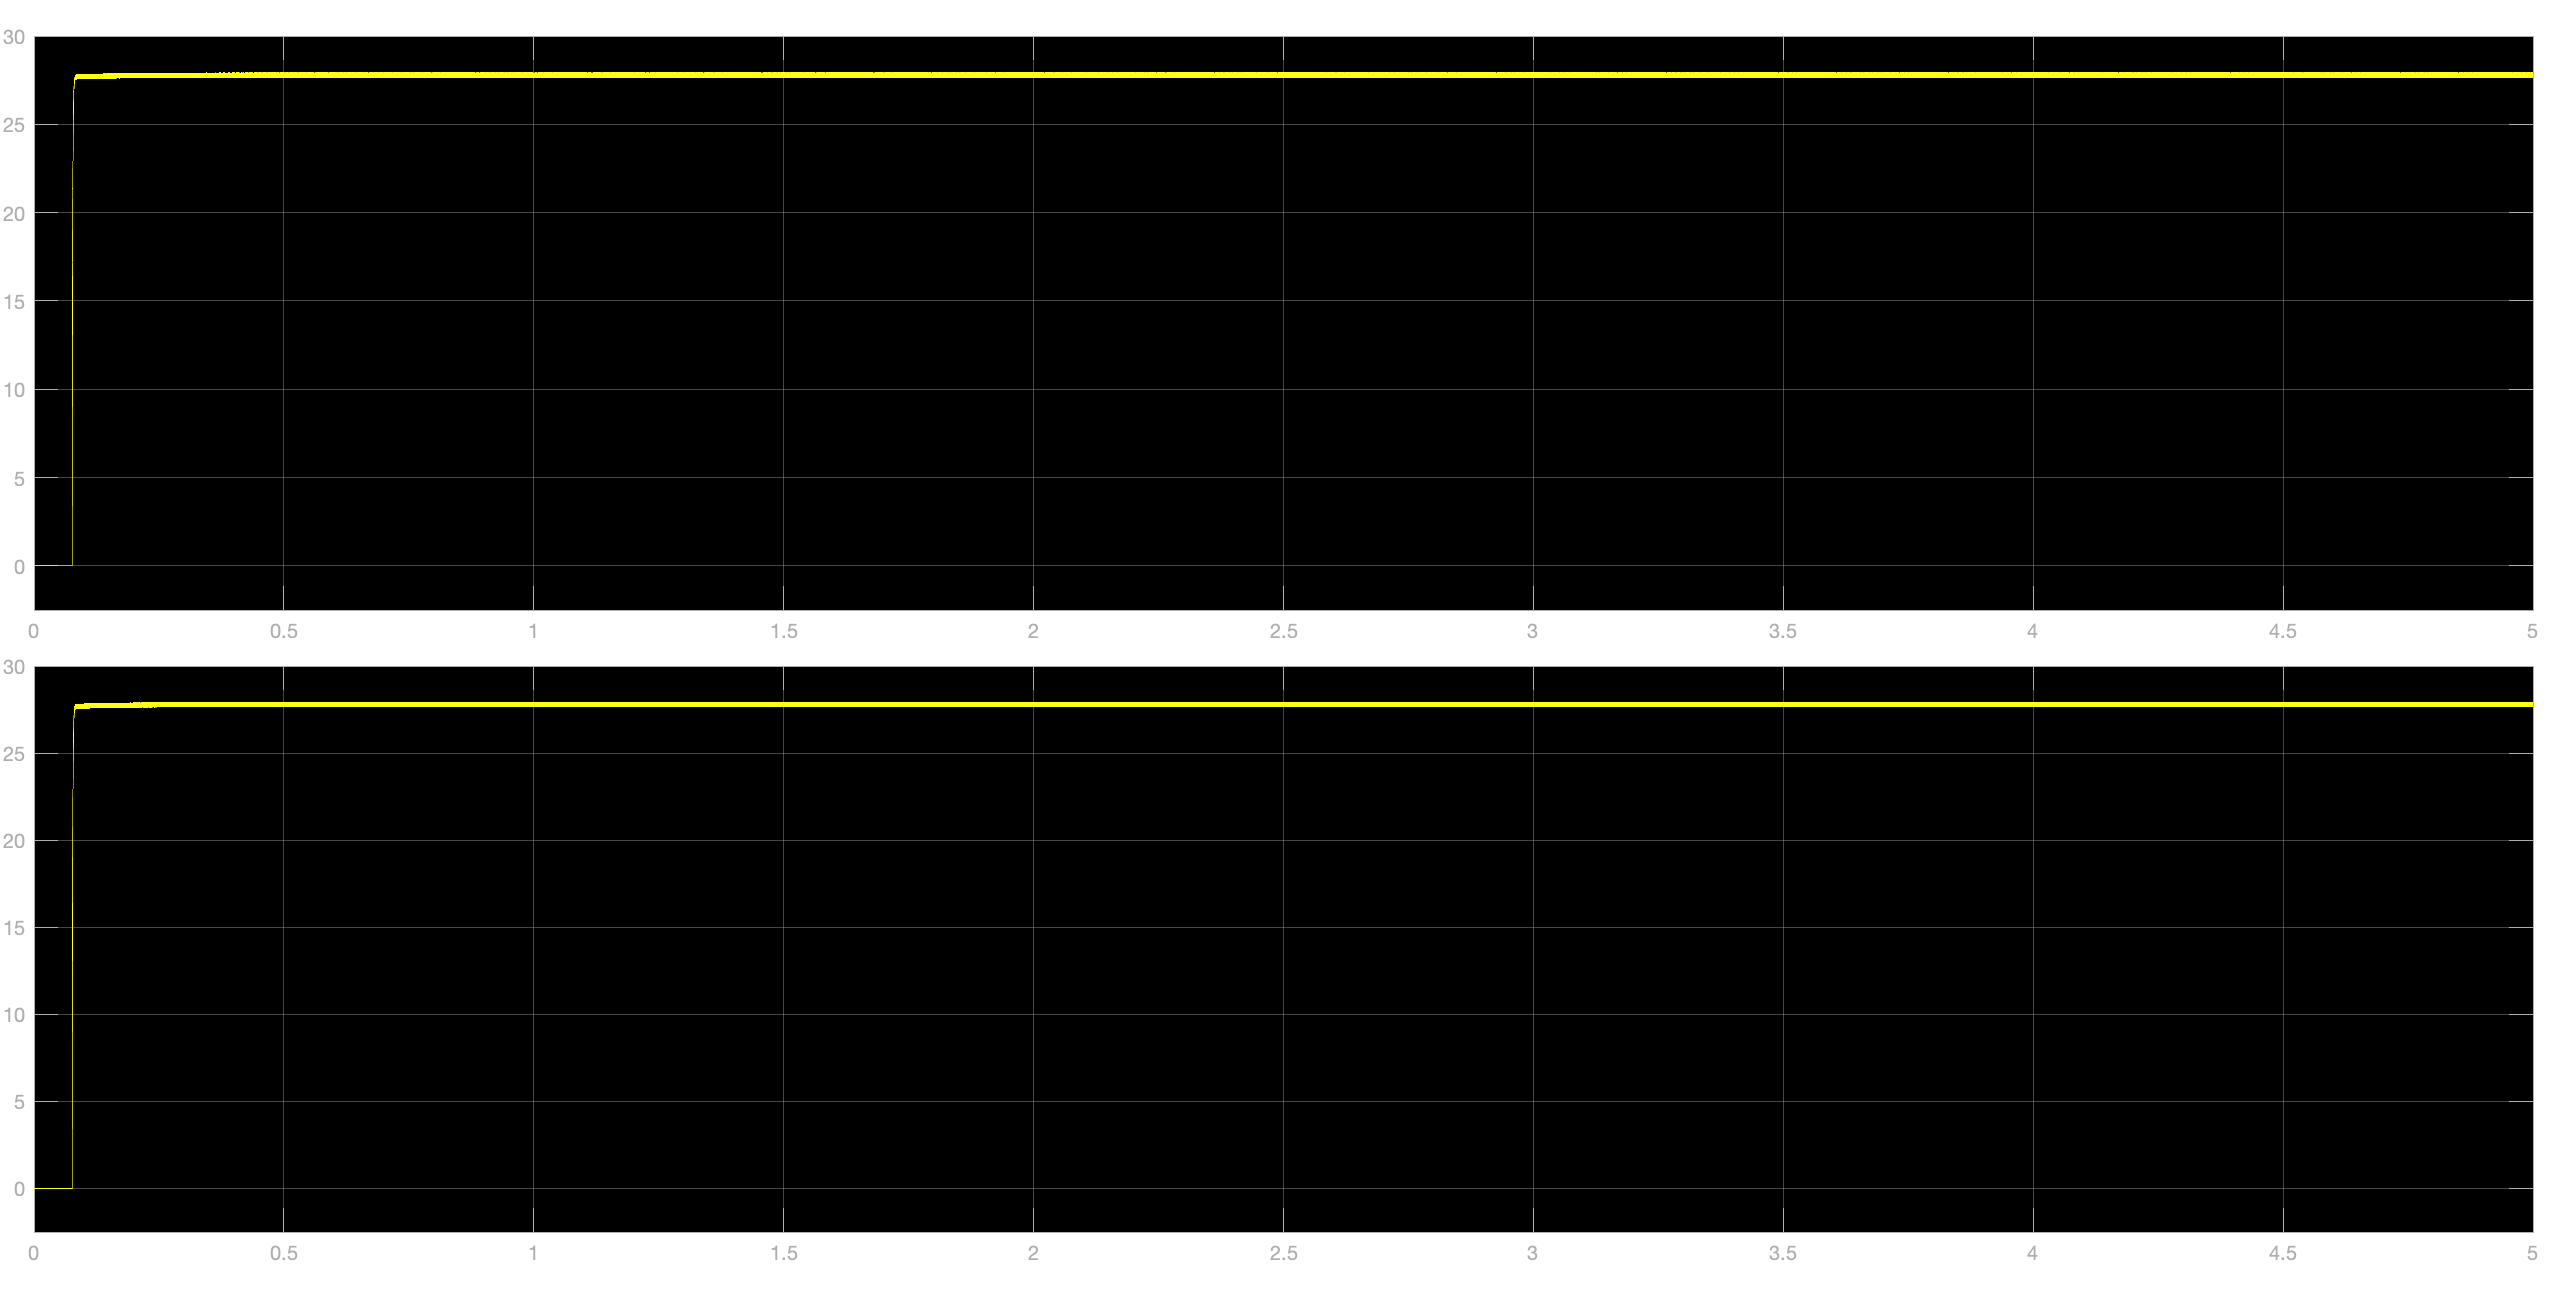
\includegraphics[trim= 0 0.255\imageheight{} 0 0, clip, width = 0.185\imageheight{}]{gl_down_load2.png}
\begin{center}
\small{Figure 2.4.2 Right DC Load Waveform}
\end{center}
\begin{center}
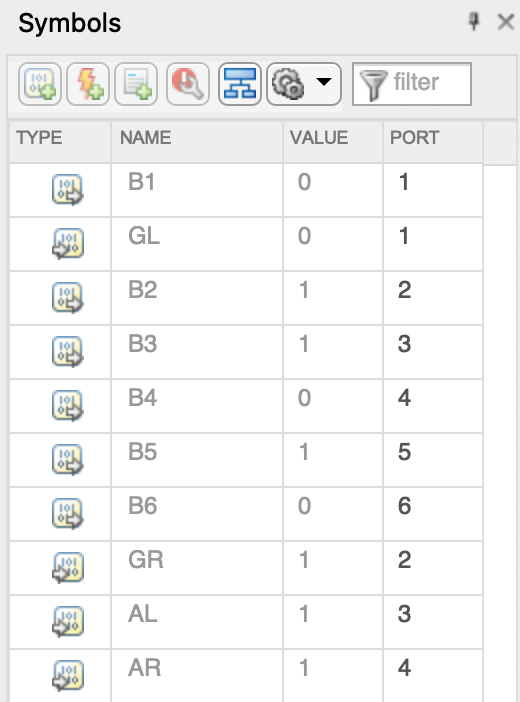
\includegraphics[width=4.5cm]{gl_down_signals.png}
\end{center}
\begin{center}
\small{Figure 2.4.3 BPCU Output Control Signals}
\end{center}
\begin{center}
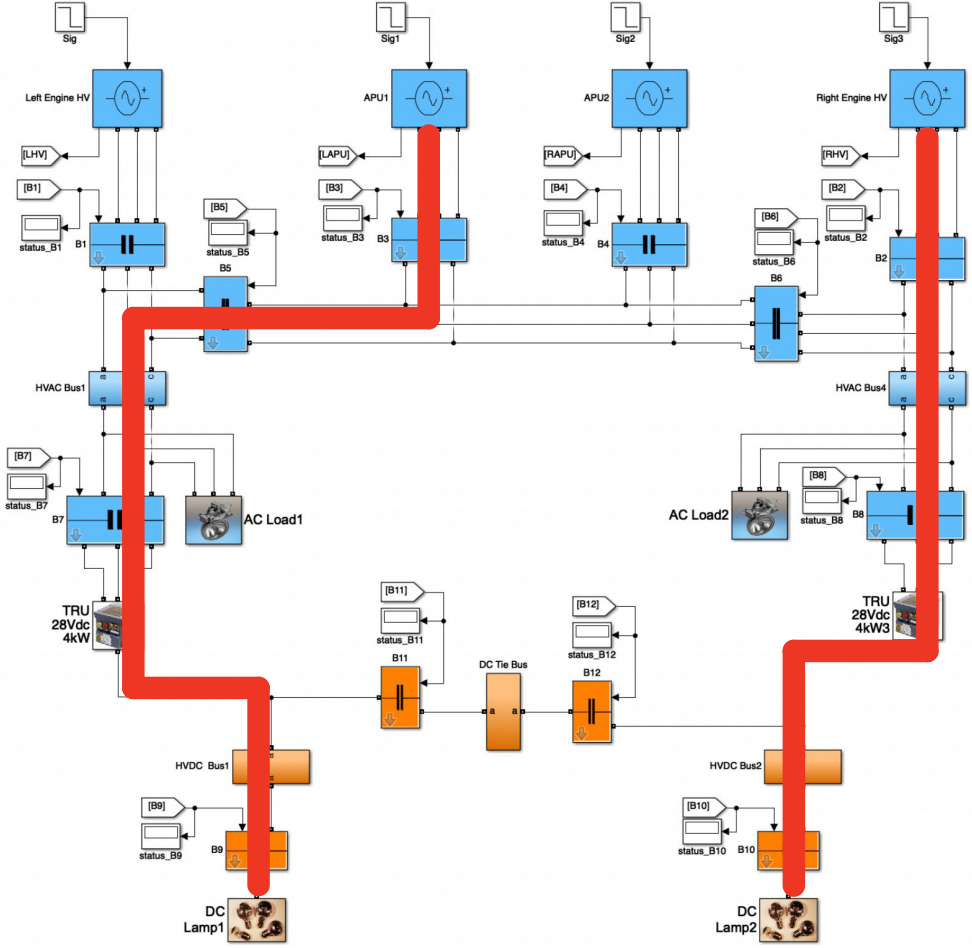
\includegraphics[width=14.5cm]{gl_down.png}
\end{center}
\begin{center}
\small{Figure 2.4.4 EPS Connection}
\end{center}
When only GL fails,  the leftmost available power supply AL empowers the left AC bus based on system guarantee G7. Only one APU, AL, is used based on system guarantee G4.
\pagebreak

\subsection{Case 4: GR, AR Not Working}
\settowidth{\imageheight}{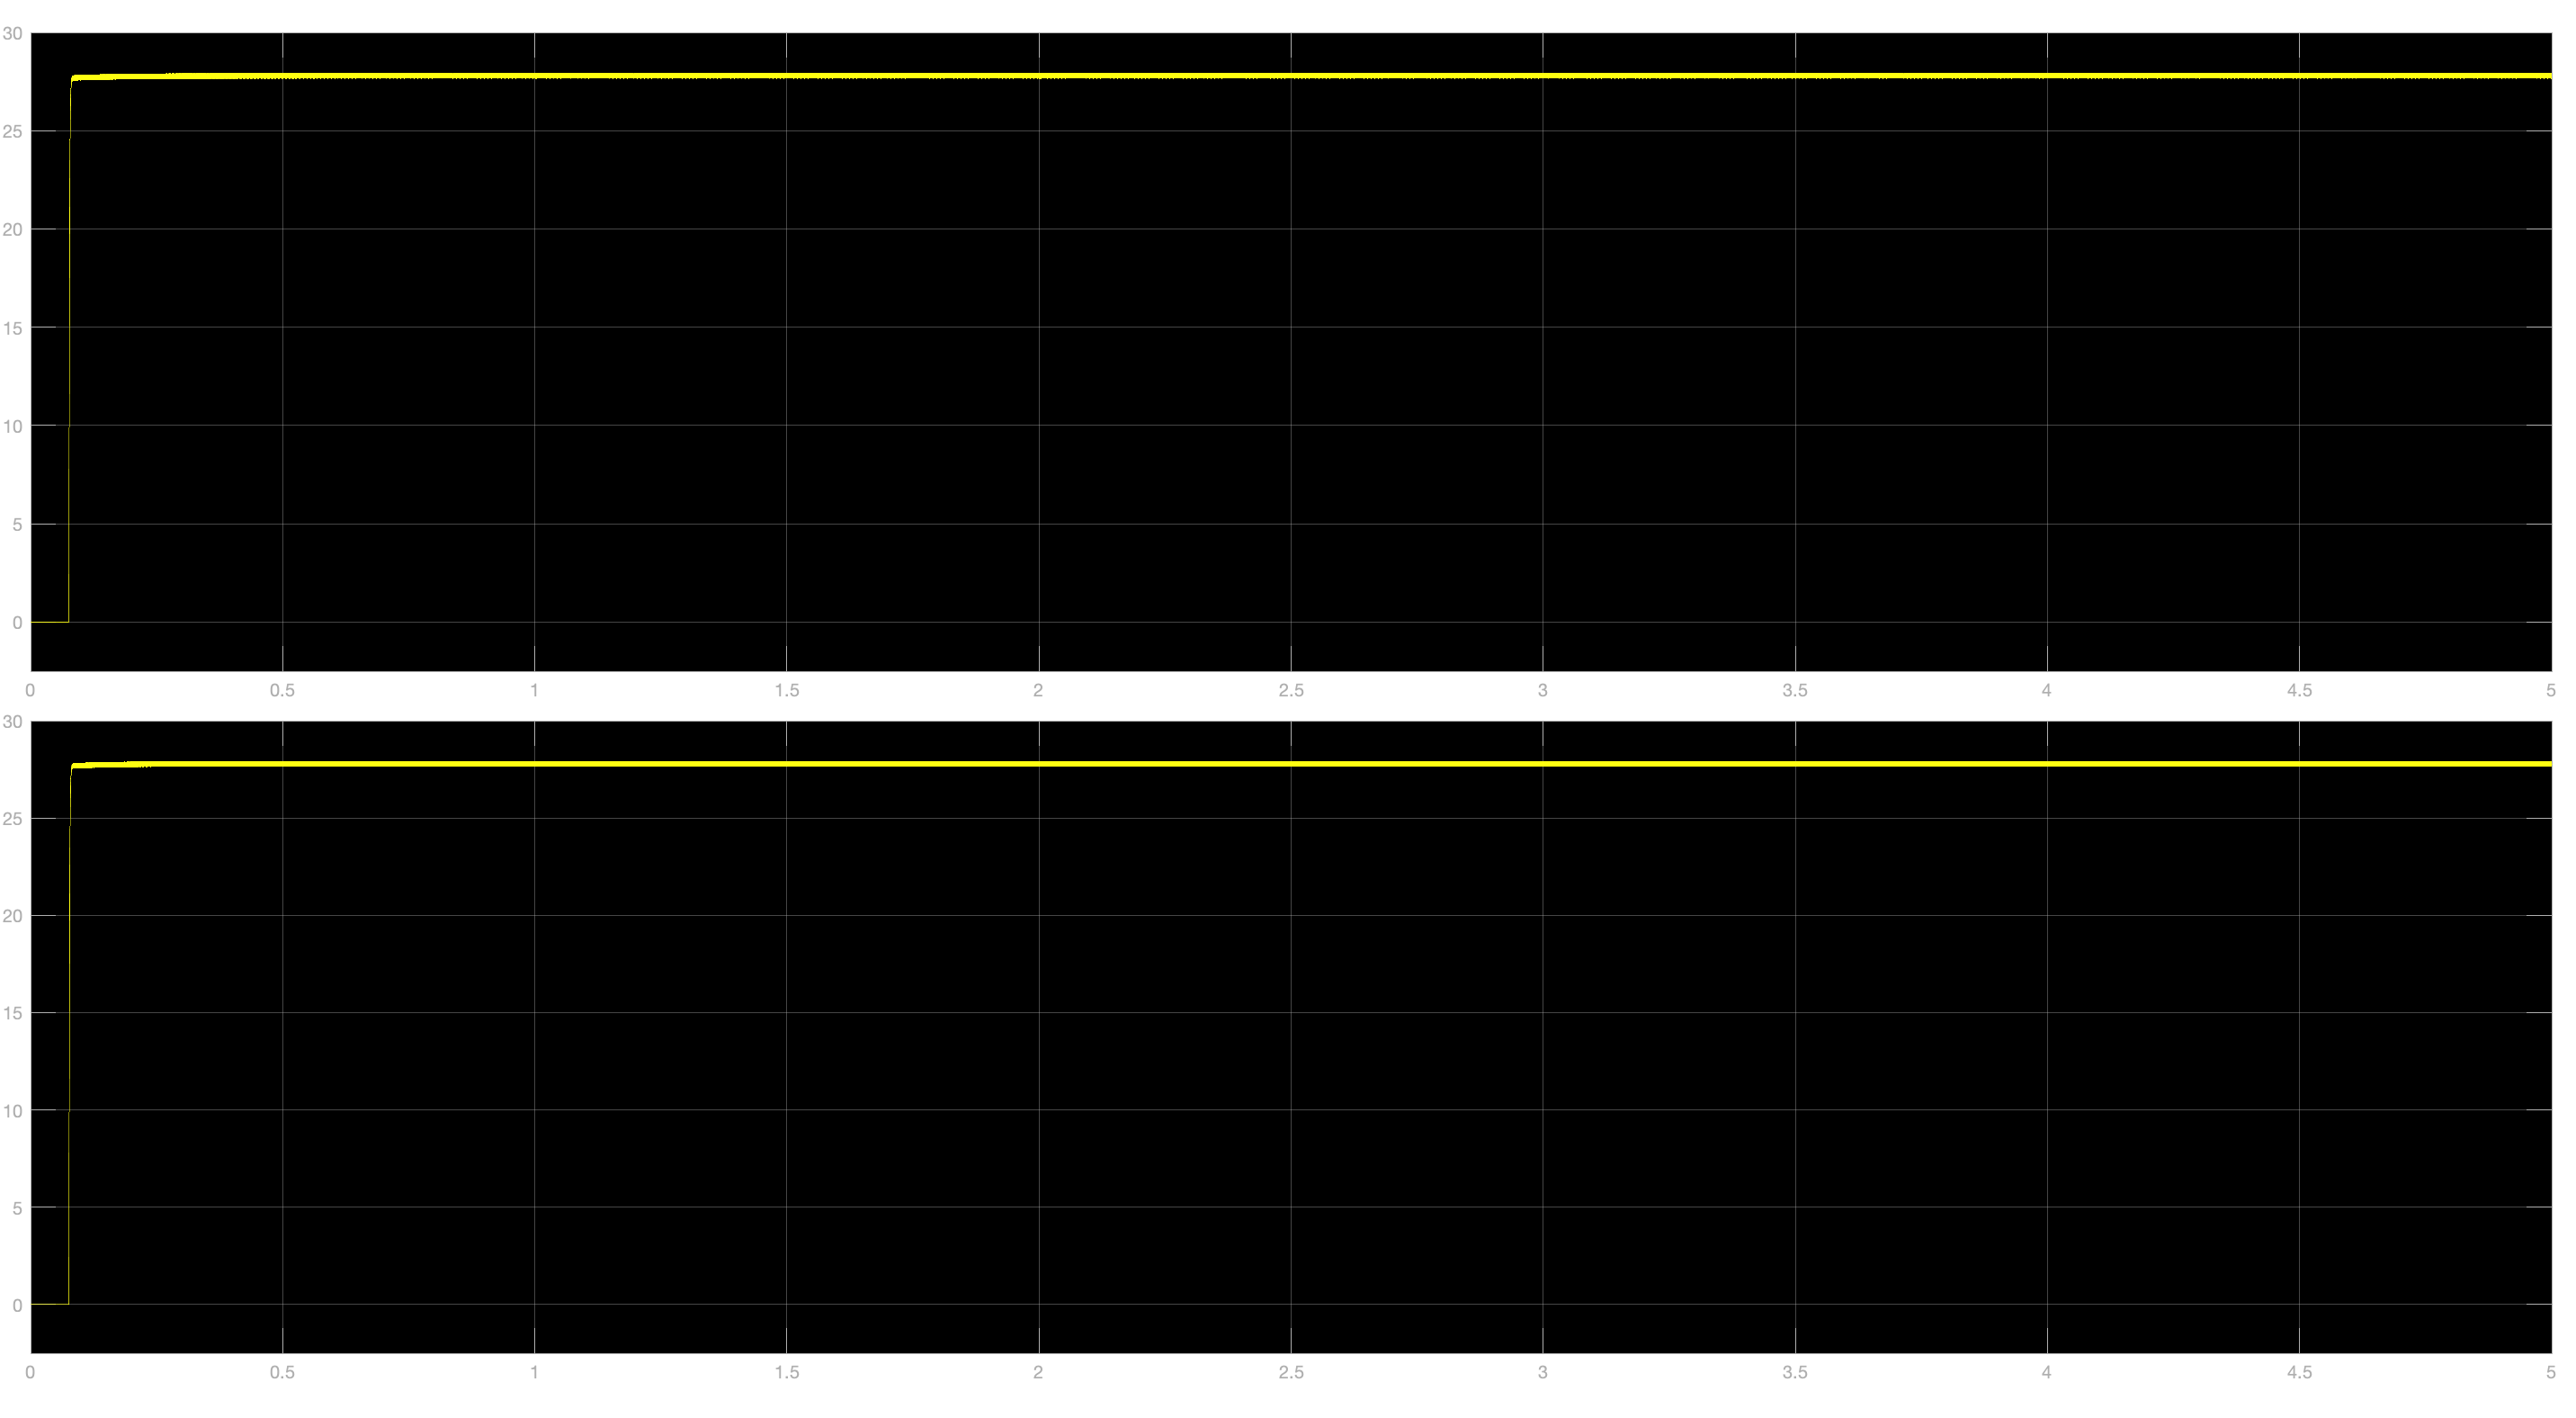
\includegraphics{gr_ar_load1.png}}
\begin{center}
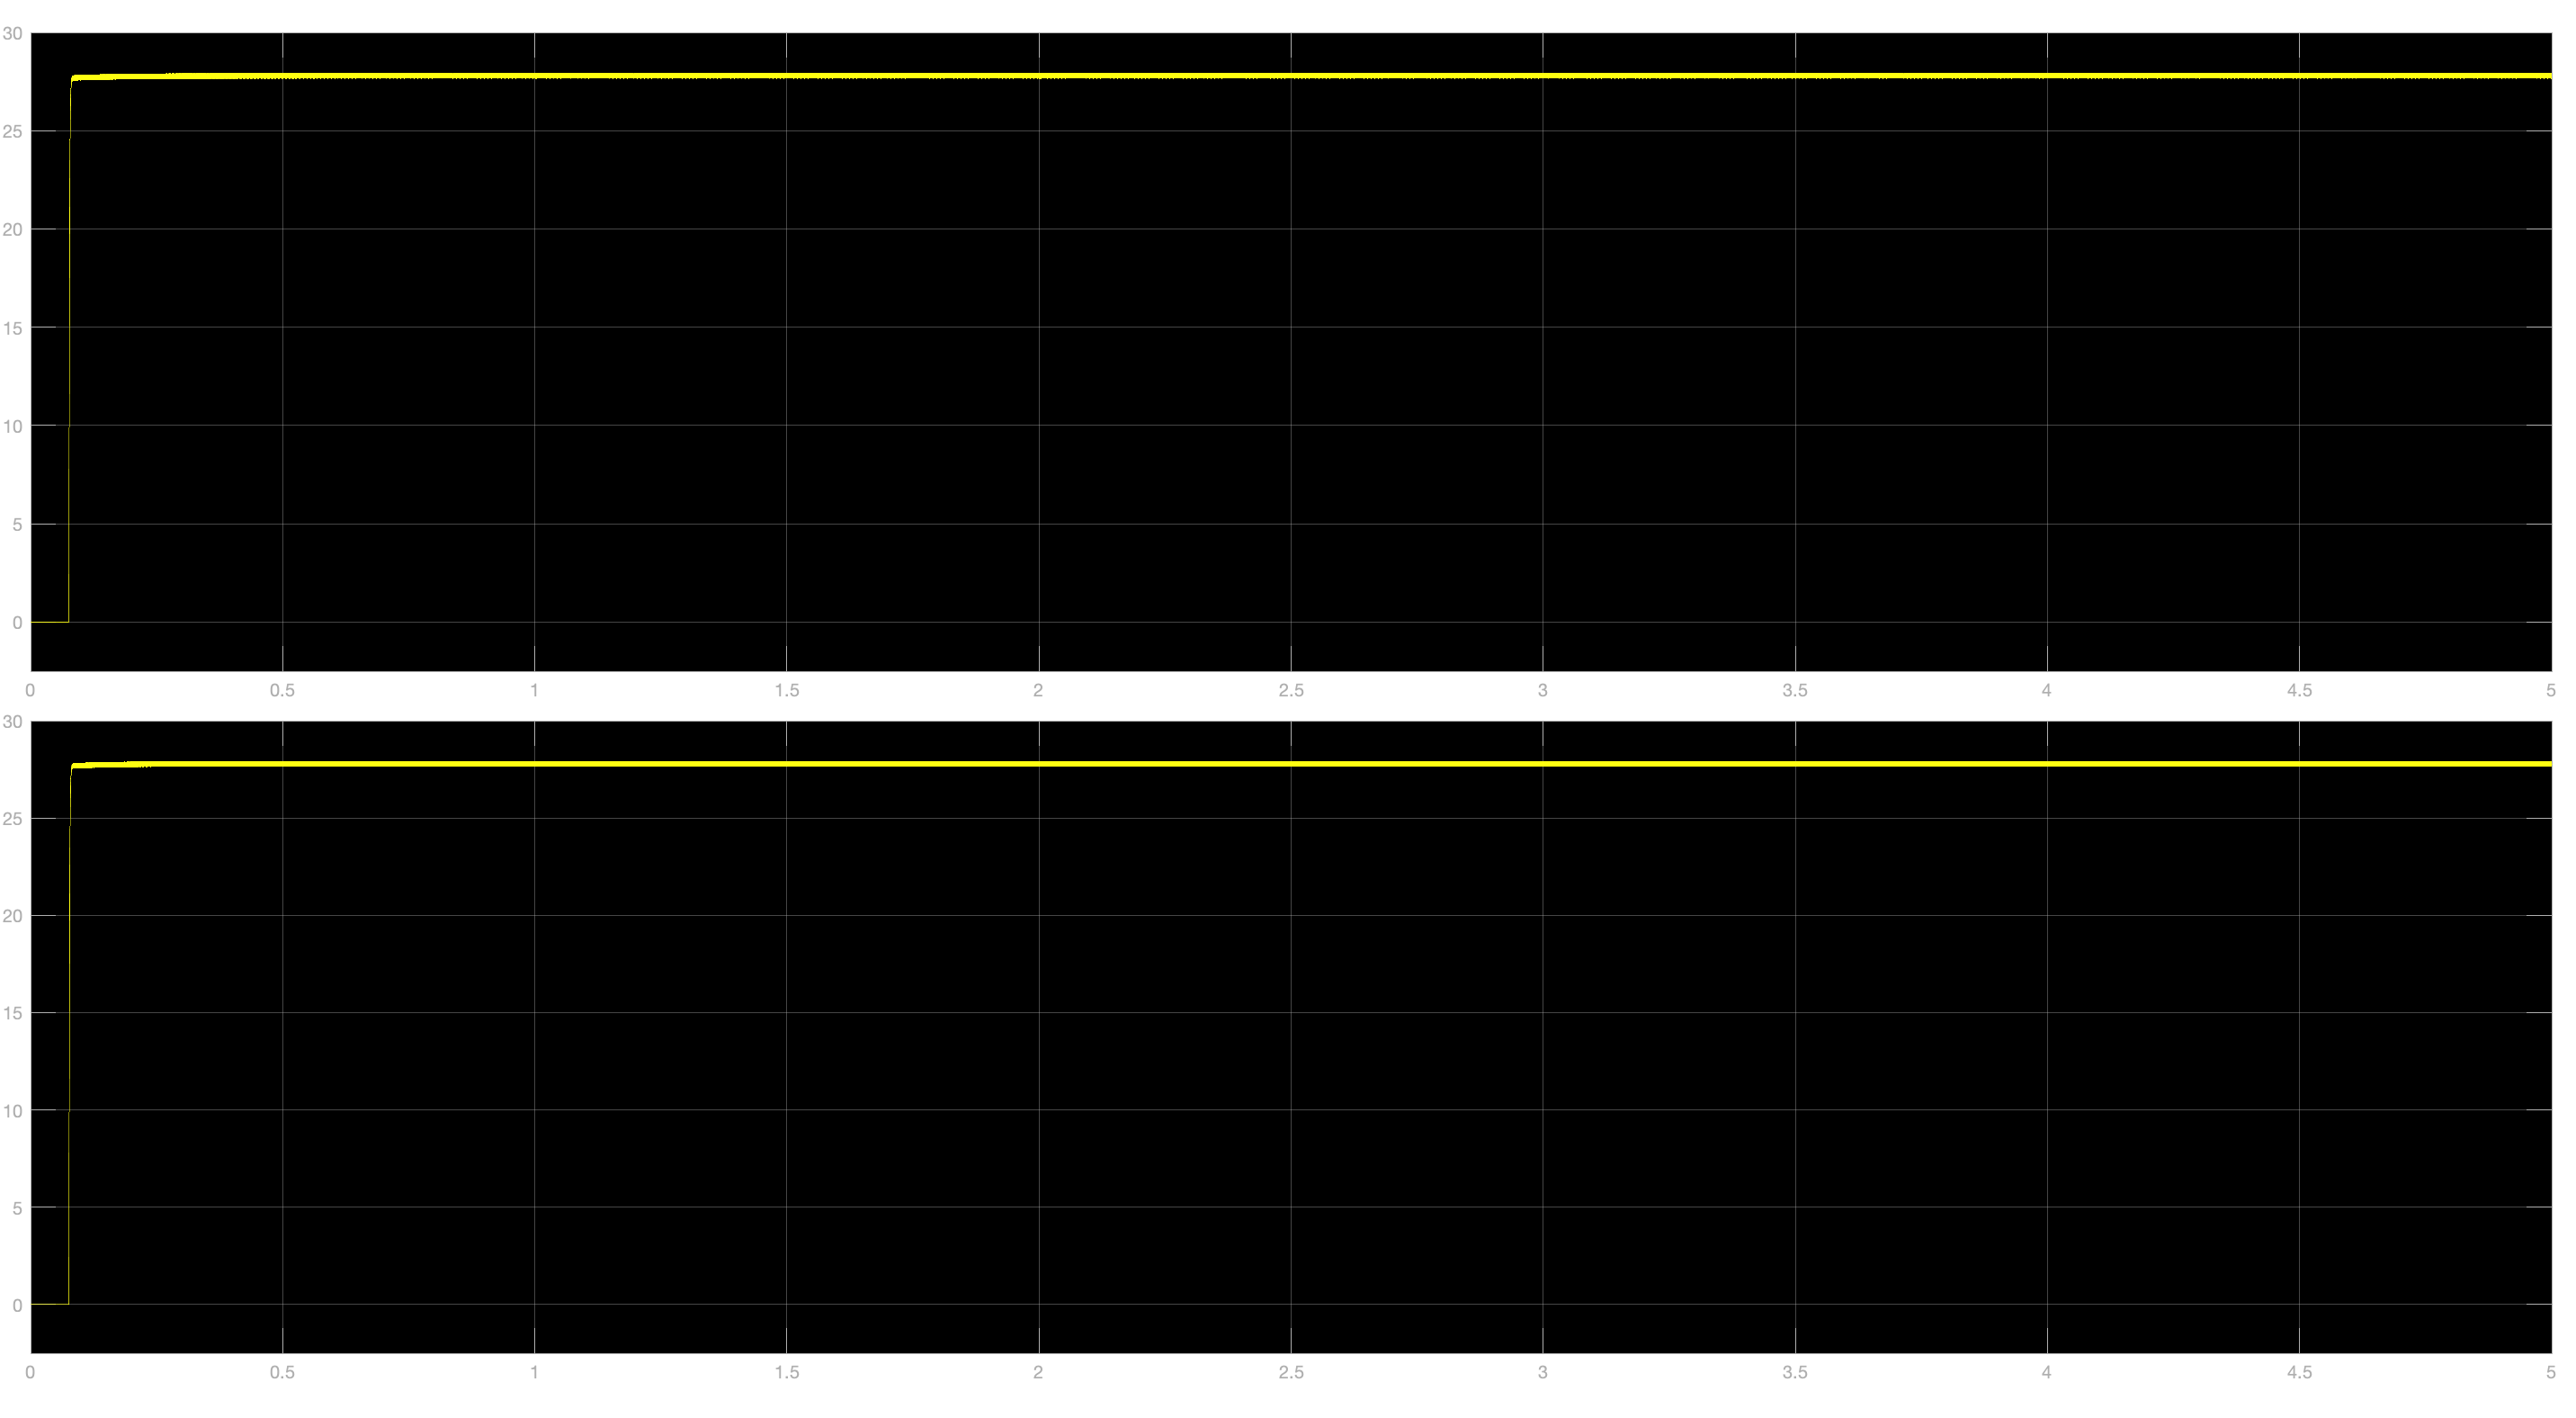
\includegraphics[trim= 0 0.28\imageheight{} 0 0, clip, width = 0.165\imageheight{}]{gr_ar_load1.png}
\end{center}
\begin{center}
\small{Figure 2.5.1 Left DC Load Waveform}
\end{center}
\settowidth{\imageheight}{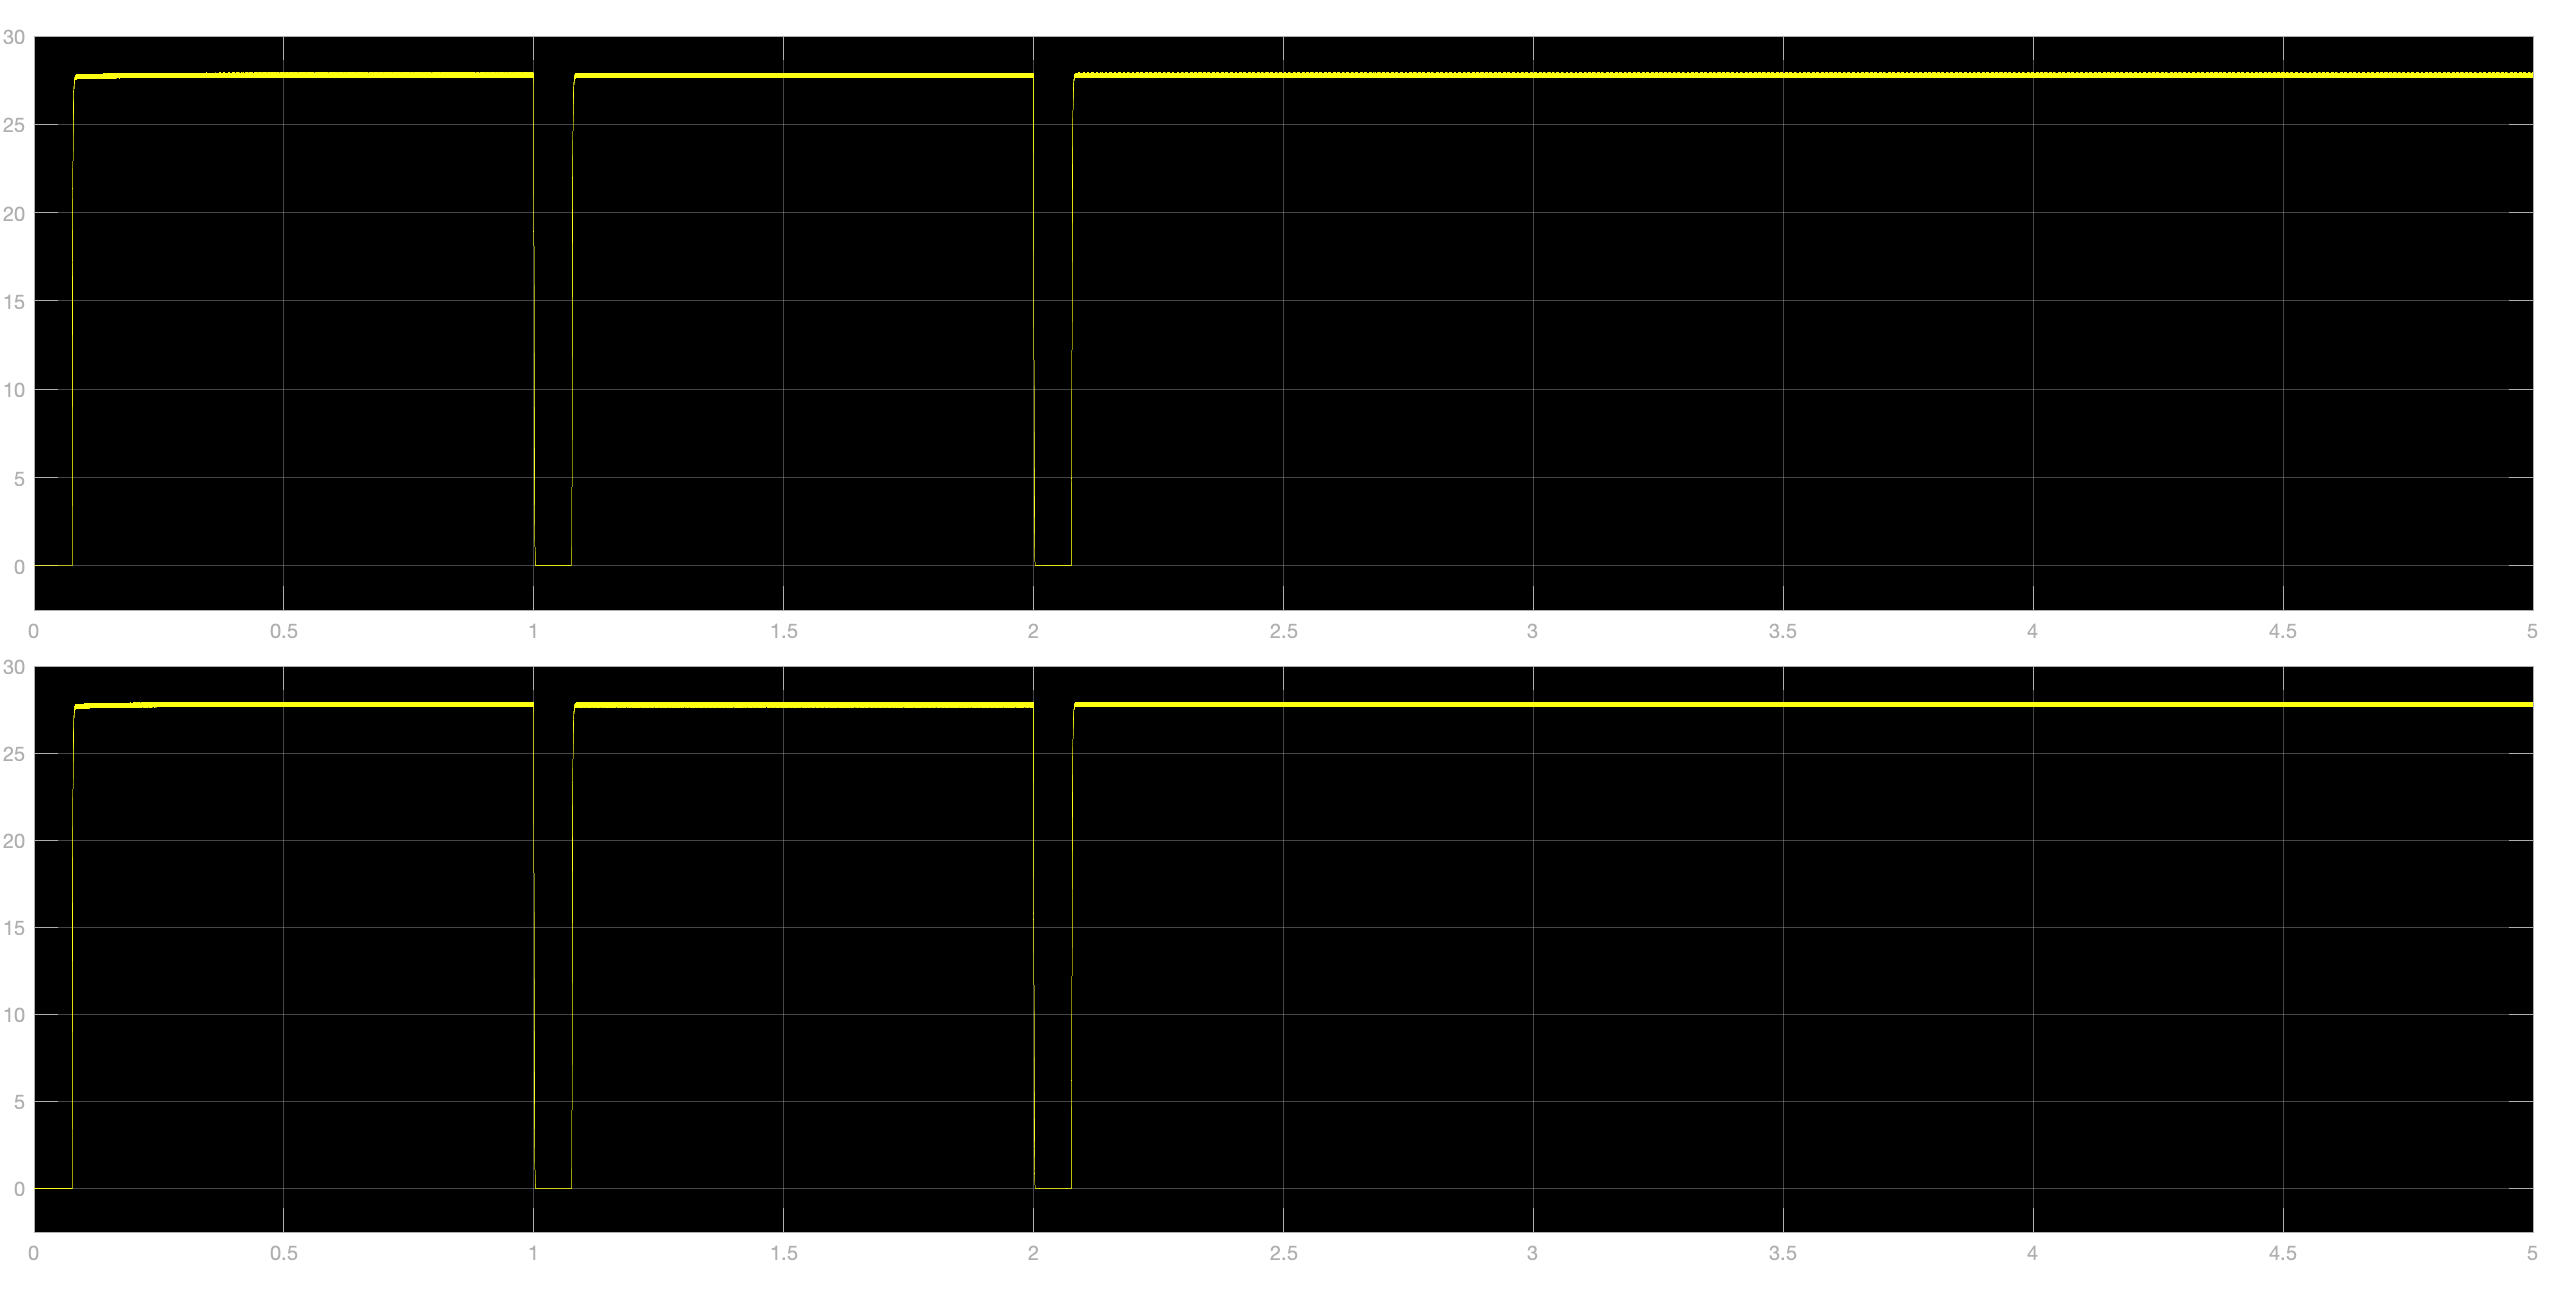
\includegraphics{gr_ar_load2.png}}
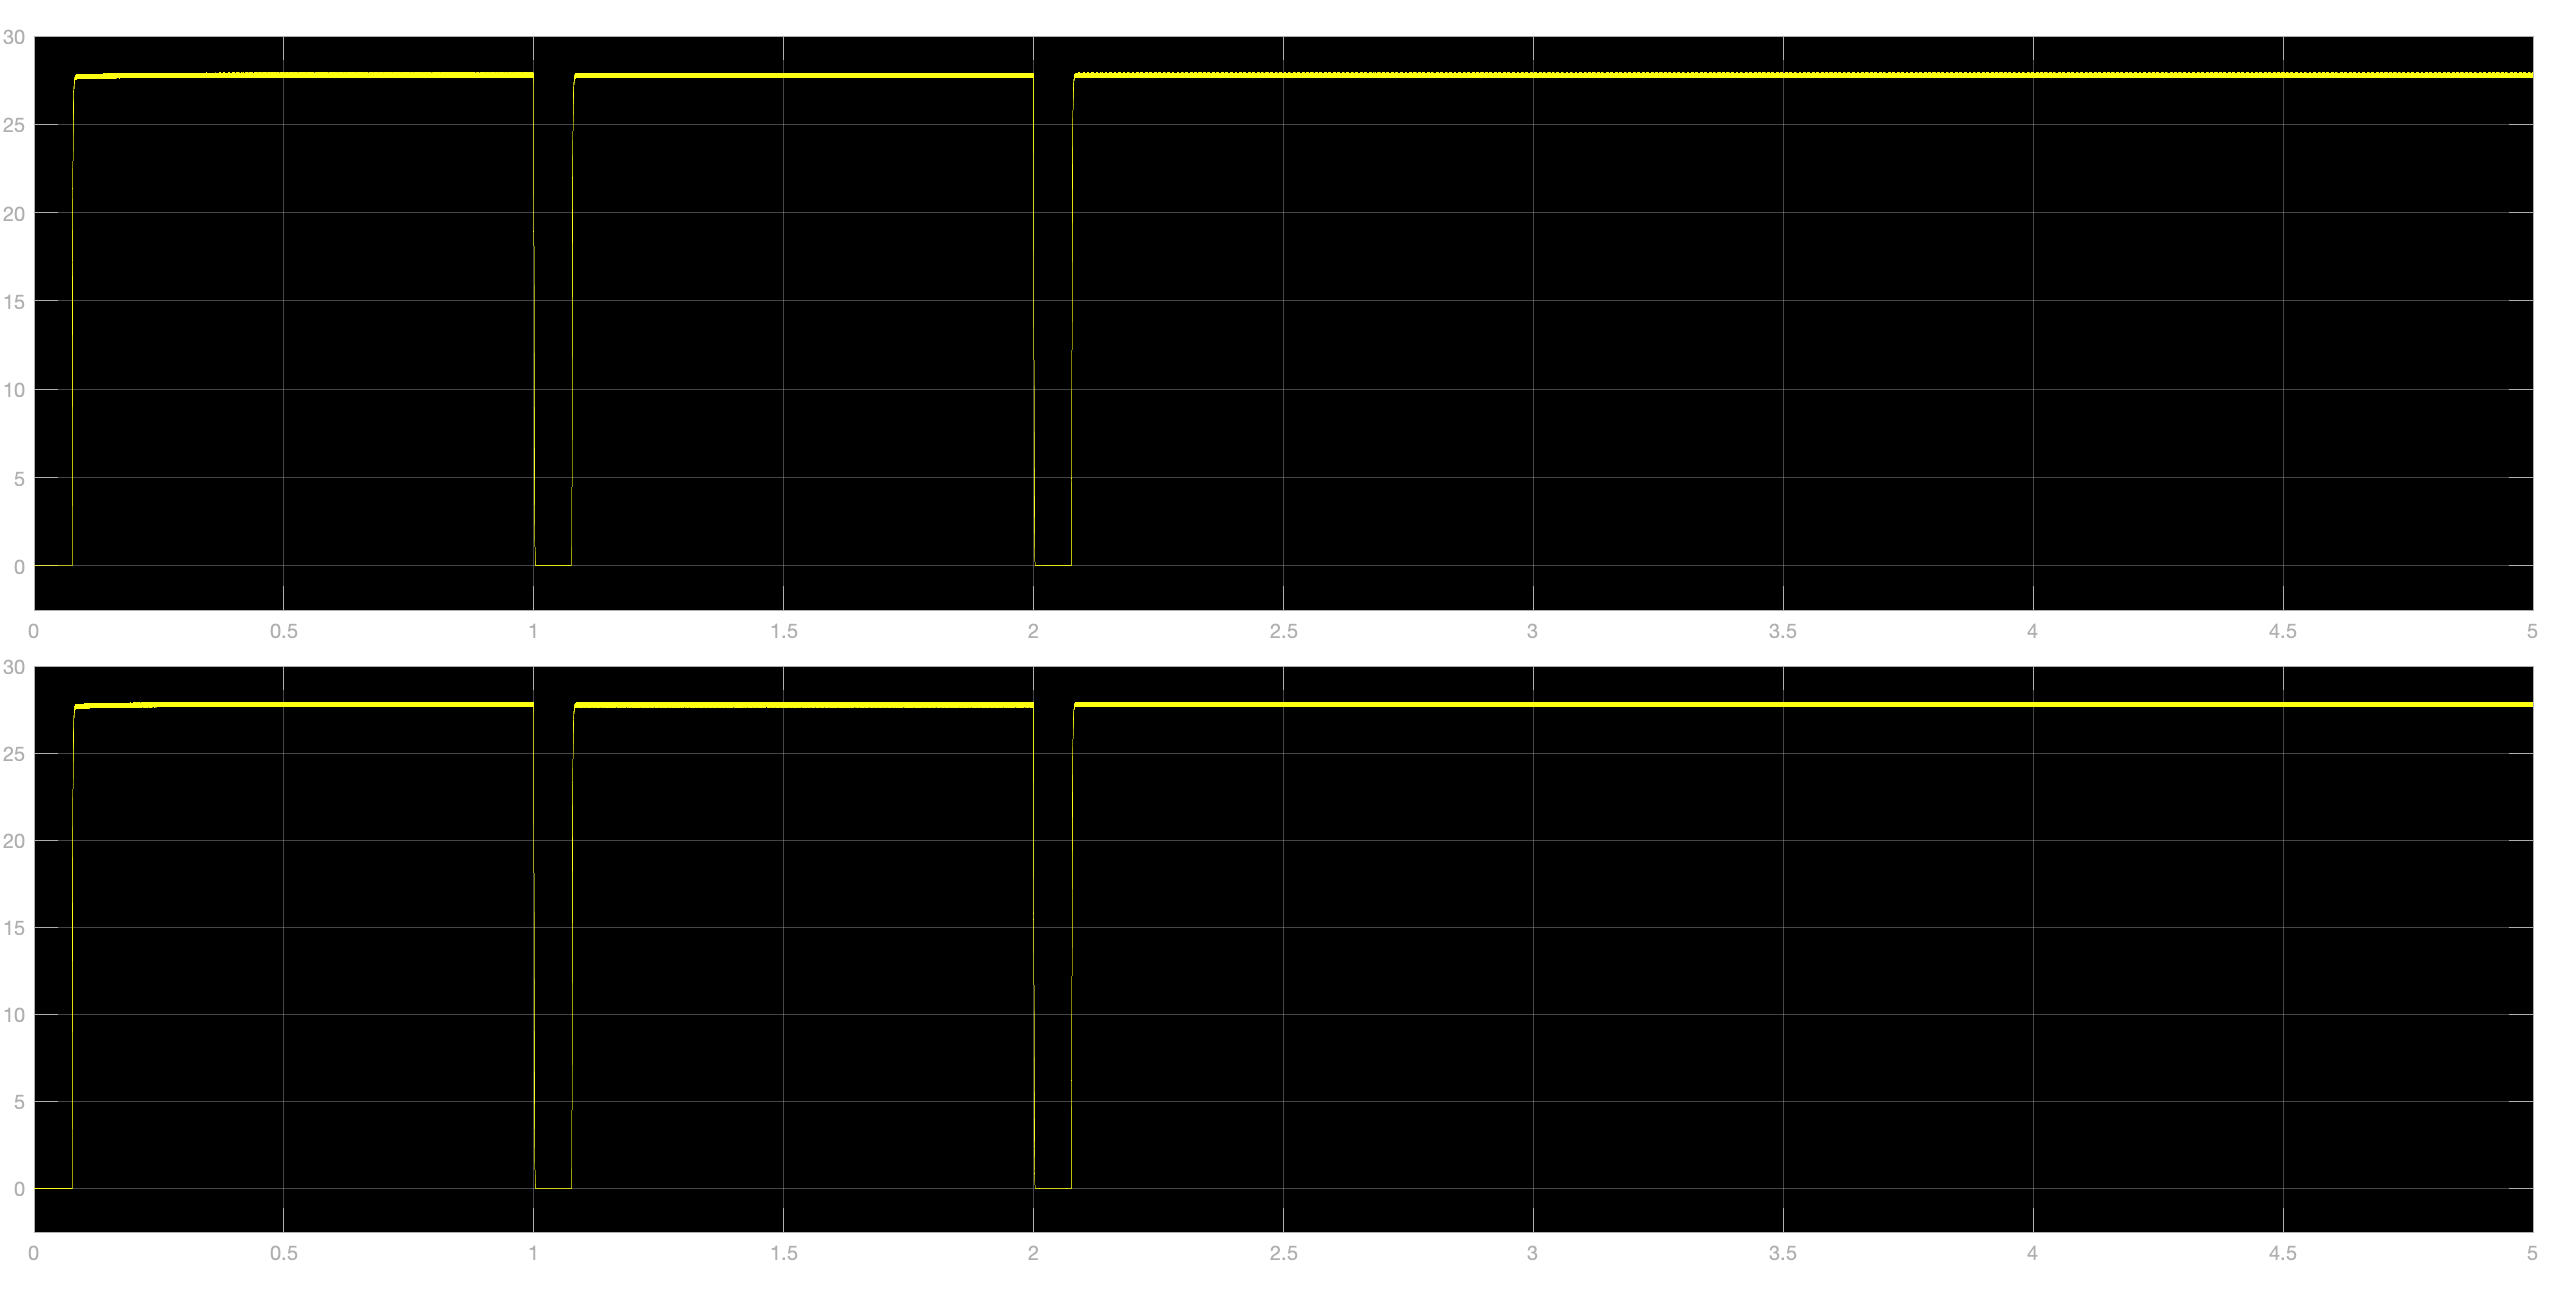
\includegraphics[trim= 0 0.255\imageheight{} 0 0, clip, width = 0.185\imageheight{}]{gr_ar_load2.png}
\begin{center}
\small{Figure 2.5.2 Right DC Load Waveform}
\end{center}
\begin{center}
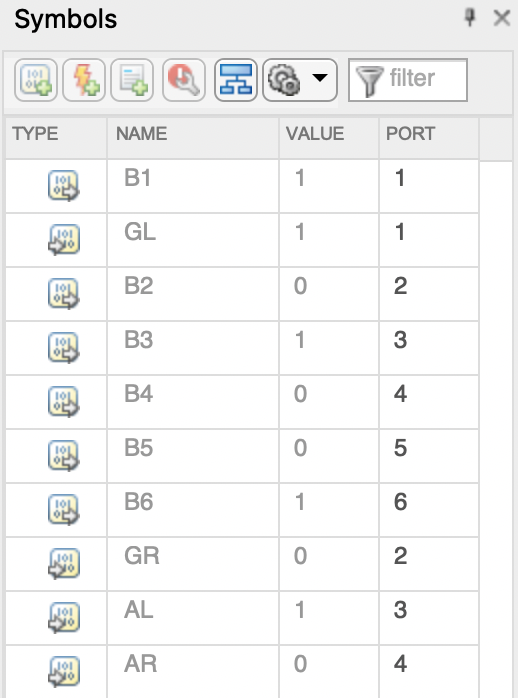
\includegraphics[width=4.5cm]{gr_ar_signals.png}
\end{center}
\begin{center}
\small{Figure 2.5.3 BPCU Output Control Signals}
\end{center}
\begin{center}
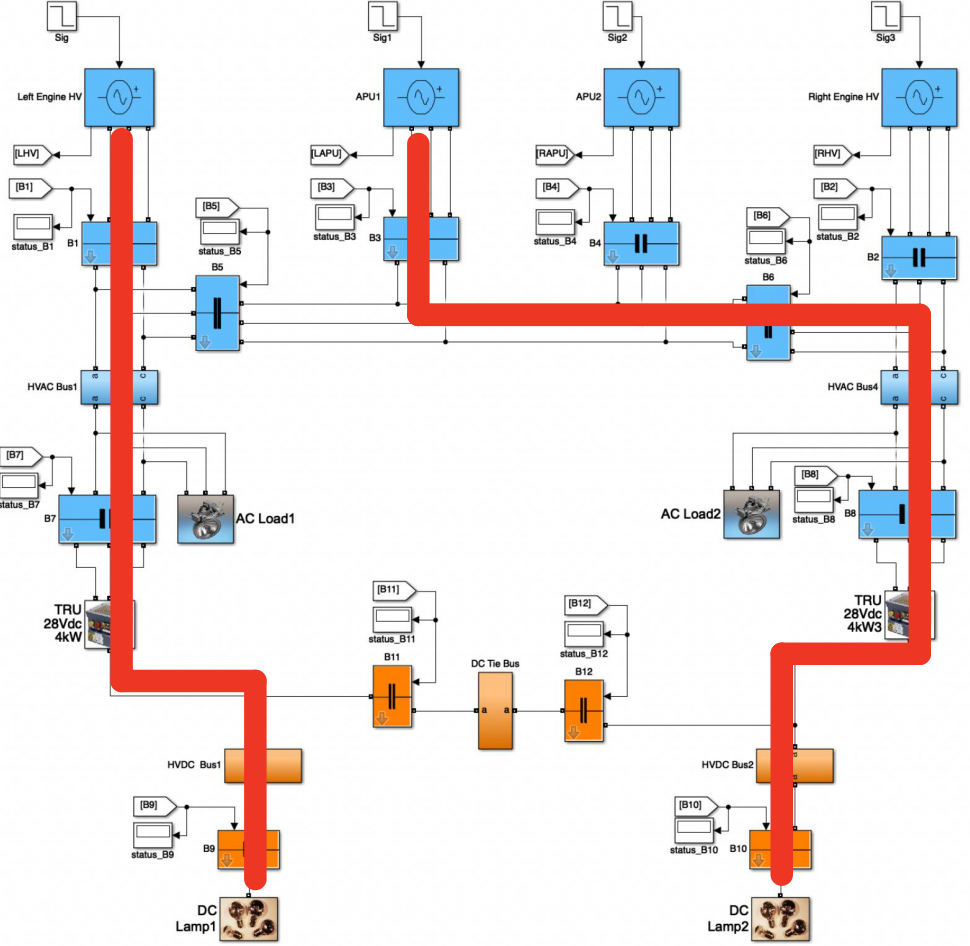
\includegraphics[width=14.5cm]{gr_ar.png}
\end{center}
\begin{center}
\small{Figure 2.5.4 EPS Connection}
\end{center}
When GR and AR fail,  the rightmost available power supply AL empowers the right AC bus based on system guarantee G8. Only one APU, AL, is used based on system guarantee G4.
\pagebreak

\subsection{Case 5: GL, AL Not Working}
\settowidth{\imageheight}{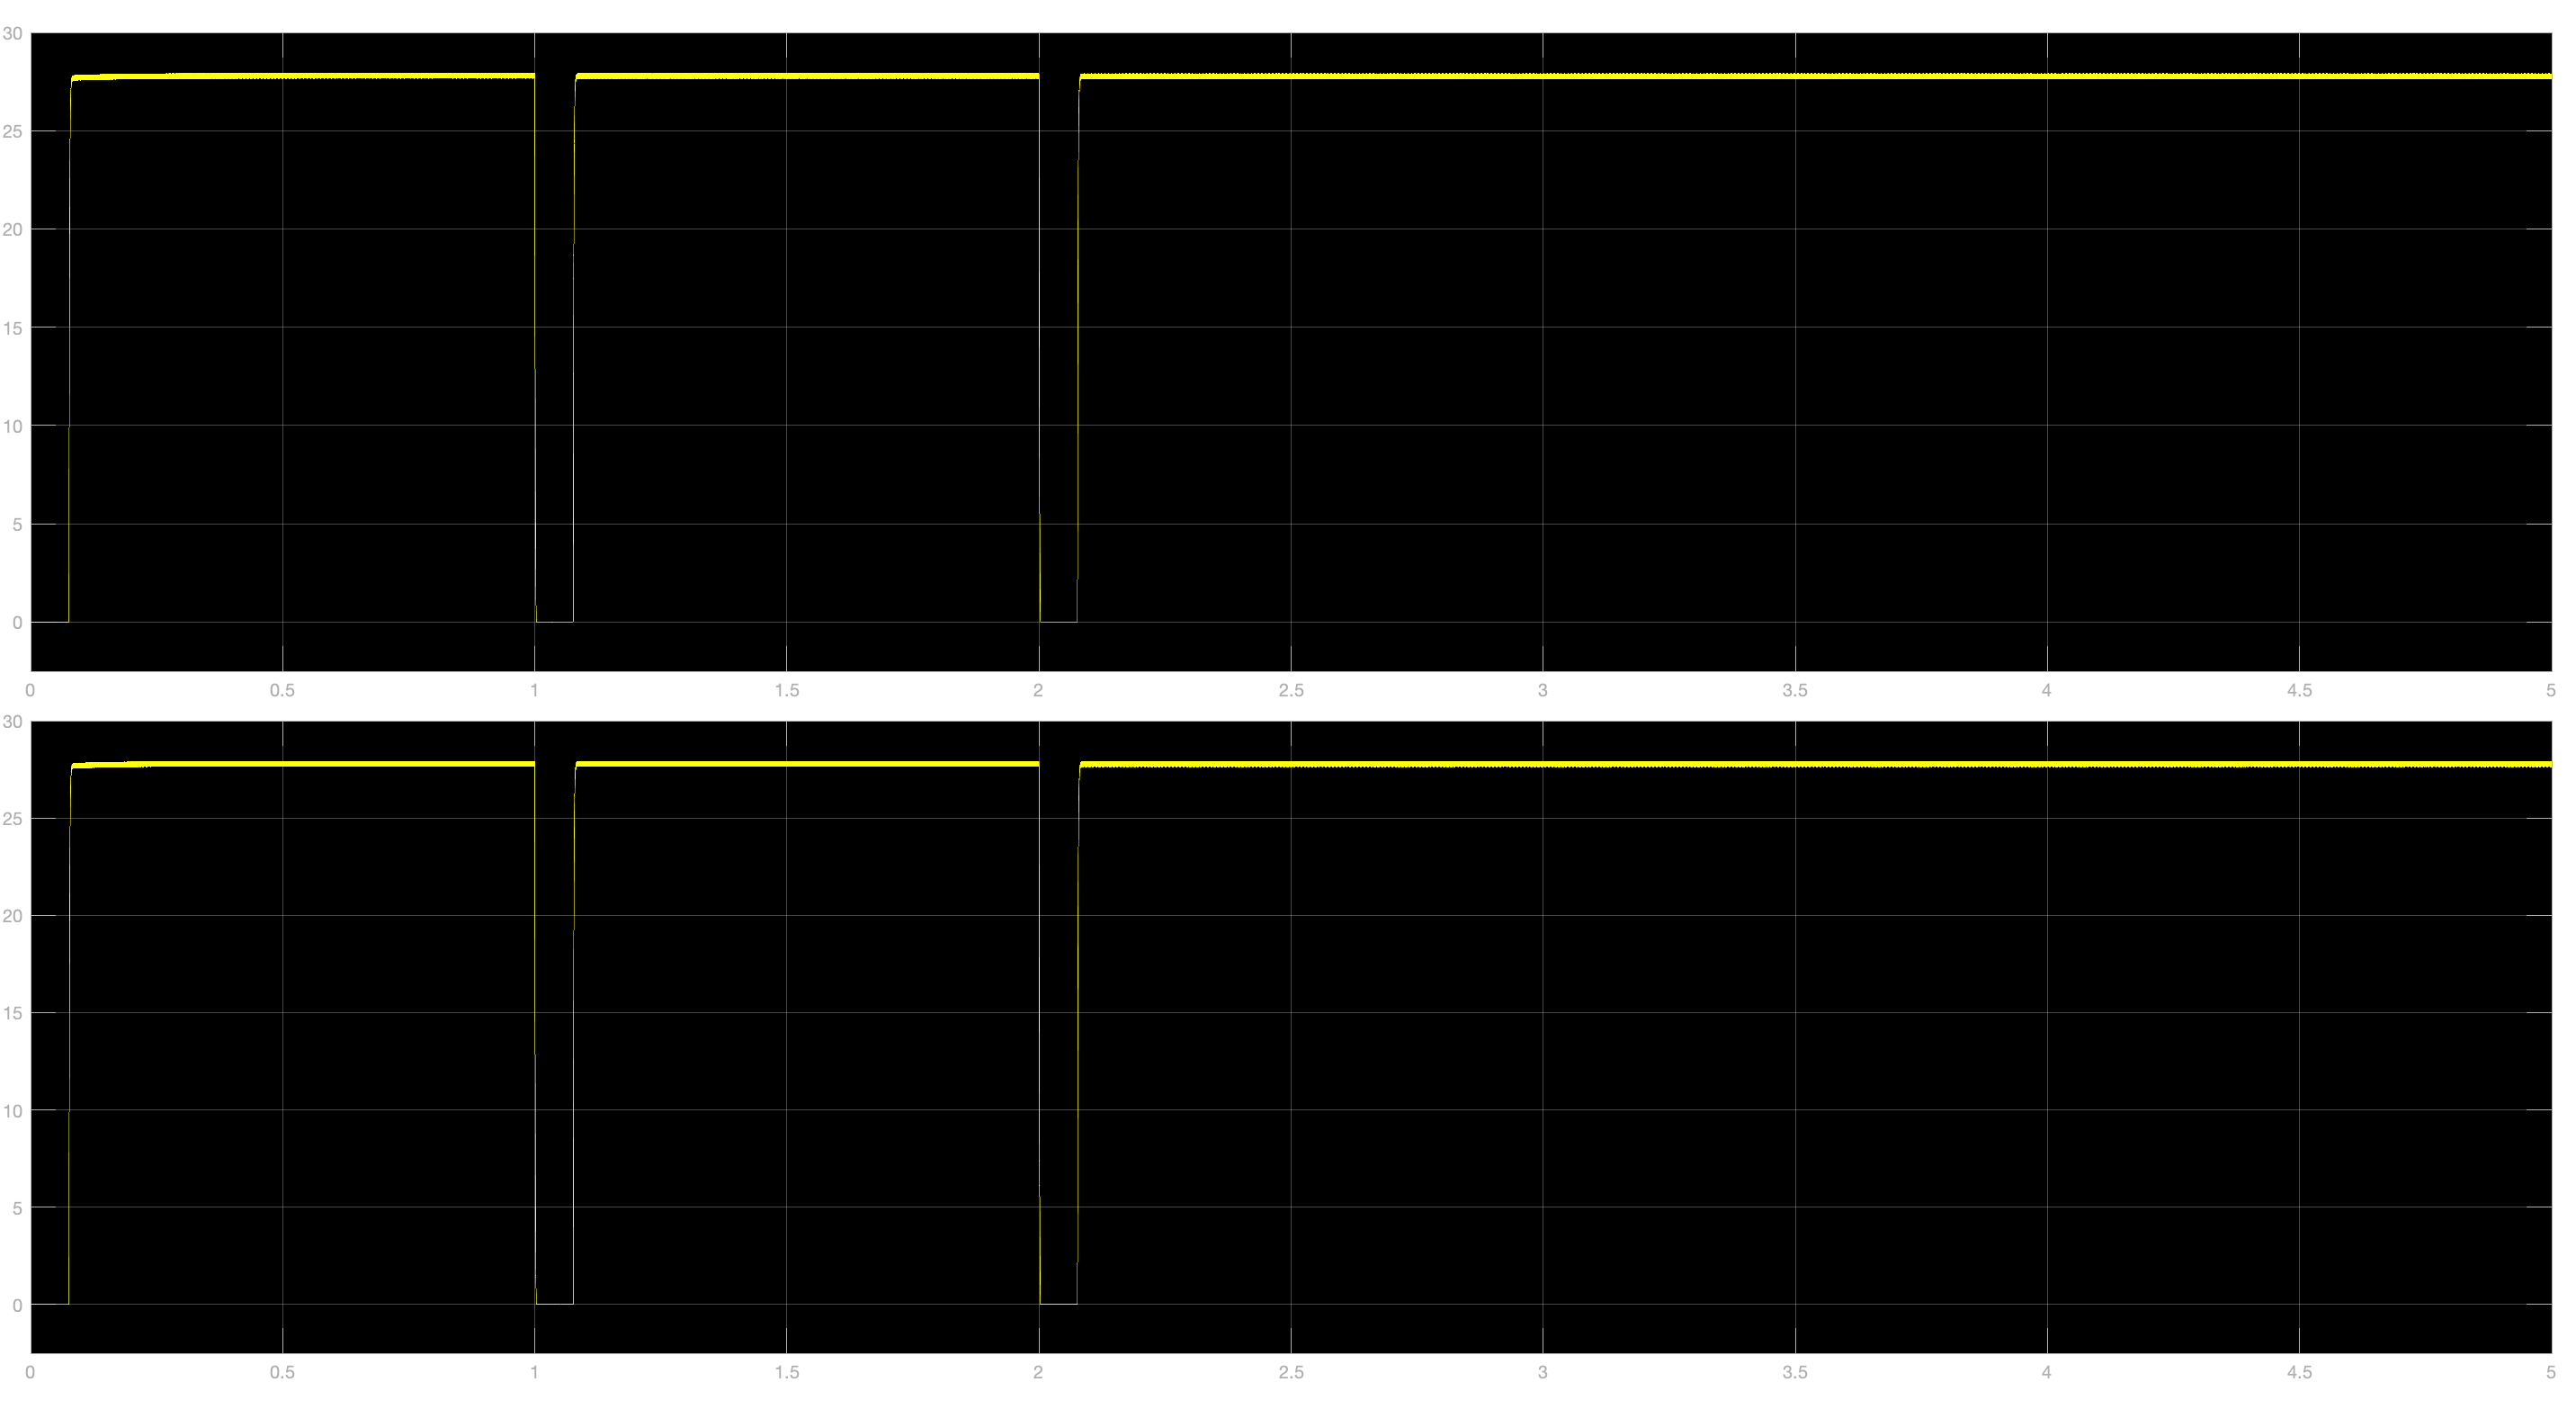
\includegraphics{gl_al_load1.png}}
\begin{center}
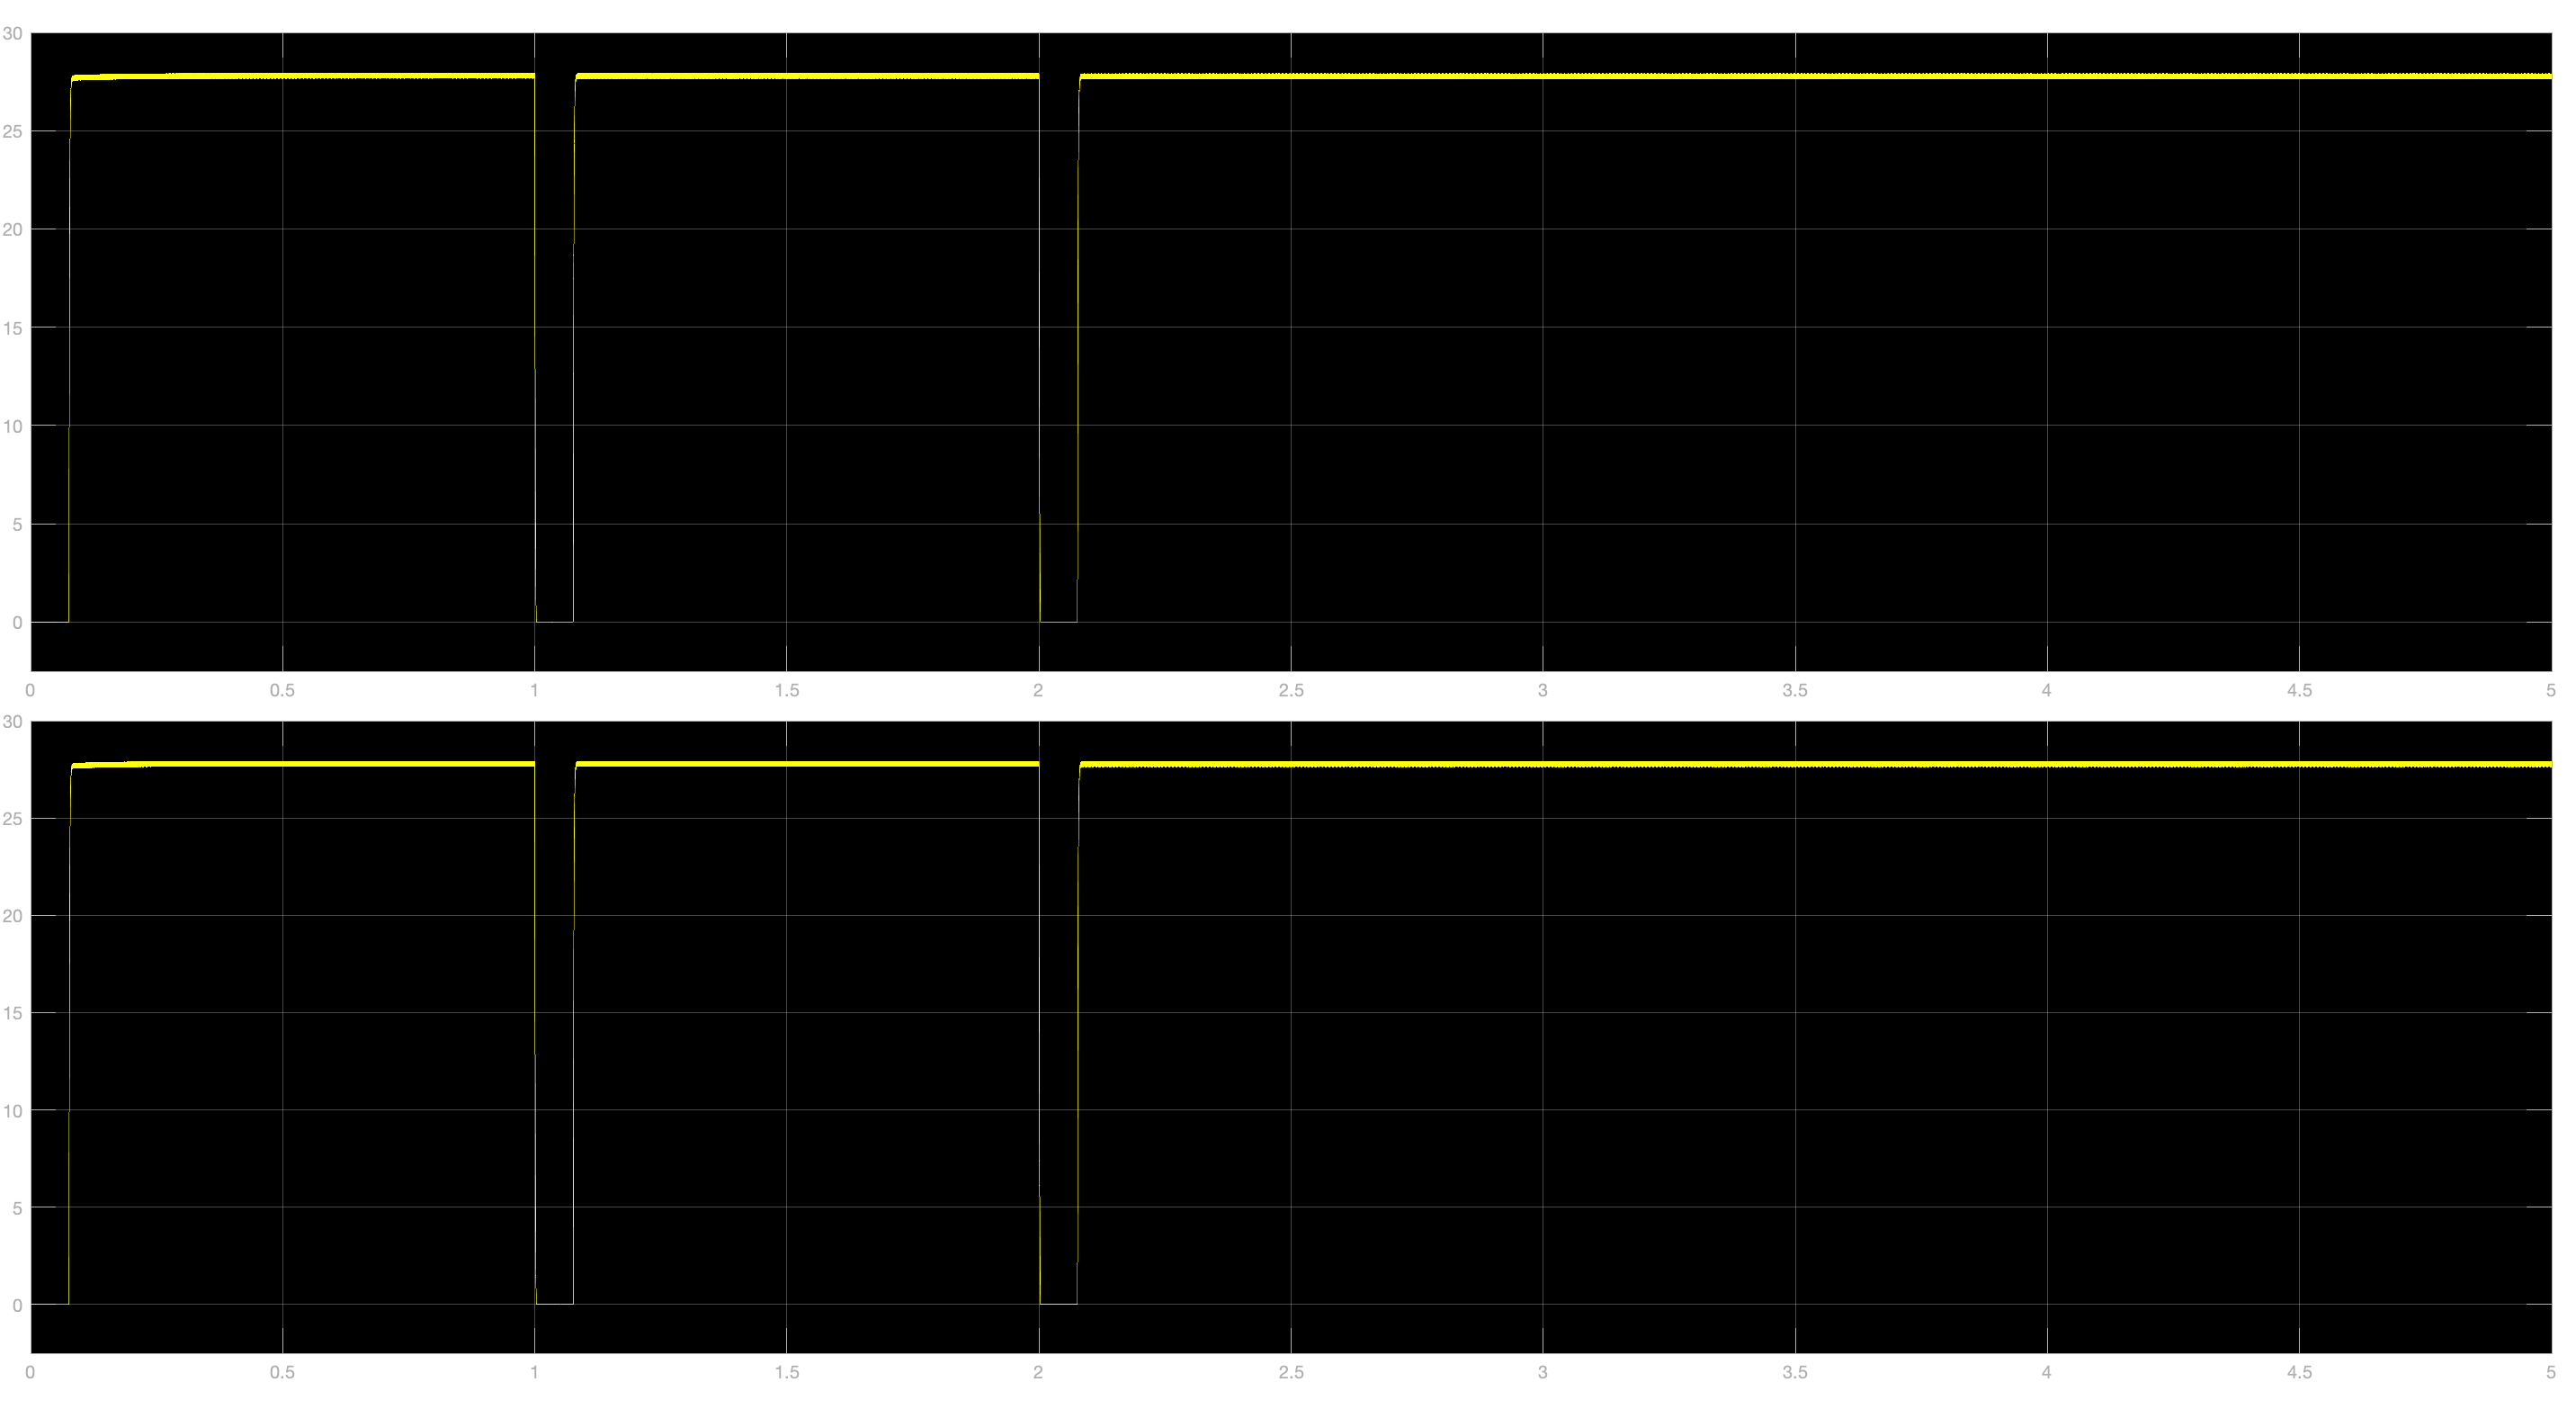
\includegraphics[trim= 0 0.28\imageheight{} 0 0, clip, width = 0.165\imageheight{}]{gl_al_load1.png}
\end{center}
\begin{center}
\small{Figure 2.6.1 Left DC Load Waveform}
\end{center}
\settowidth{\imageheight}{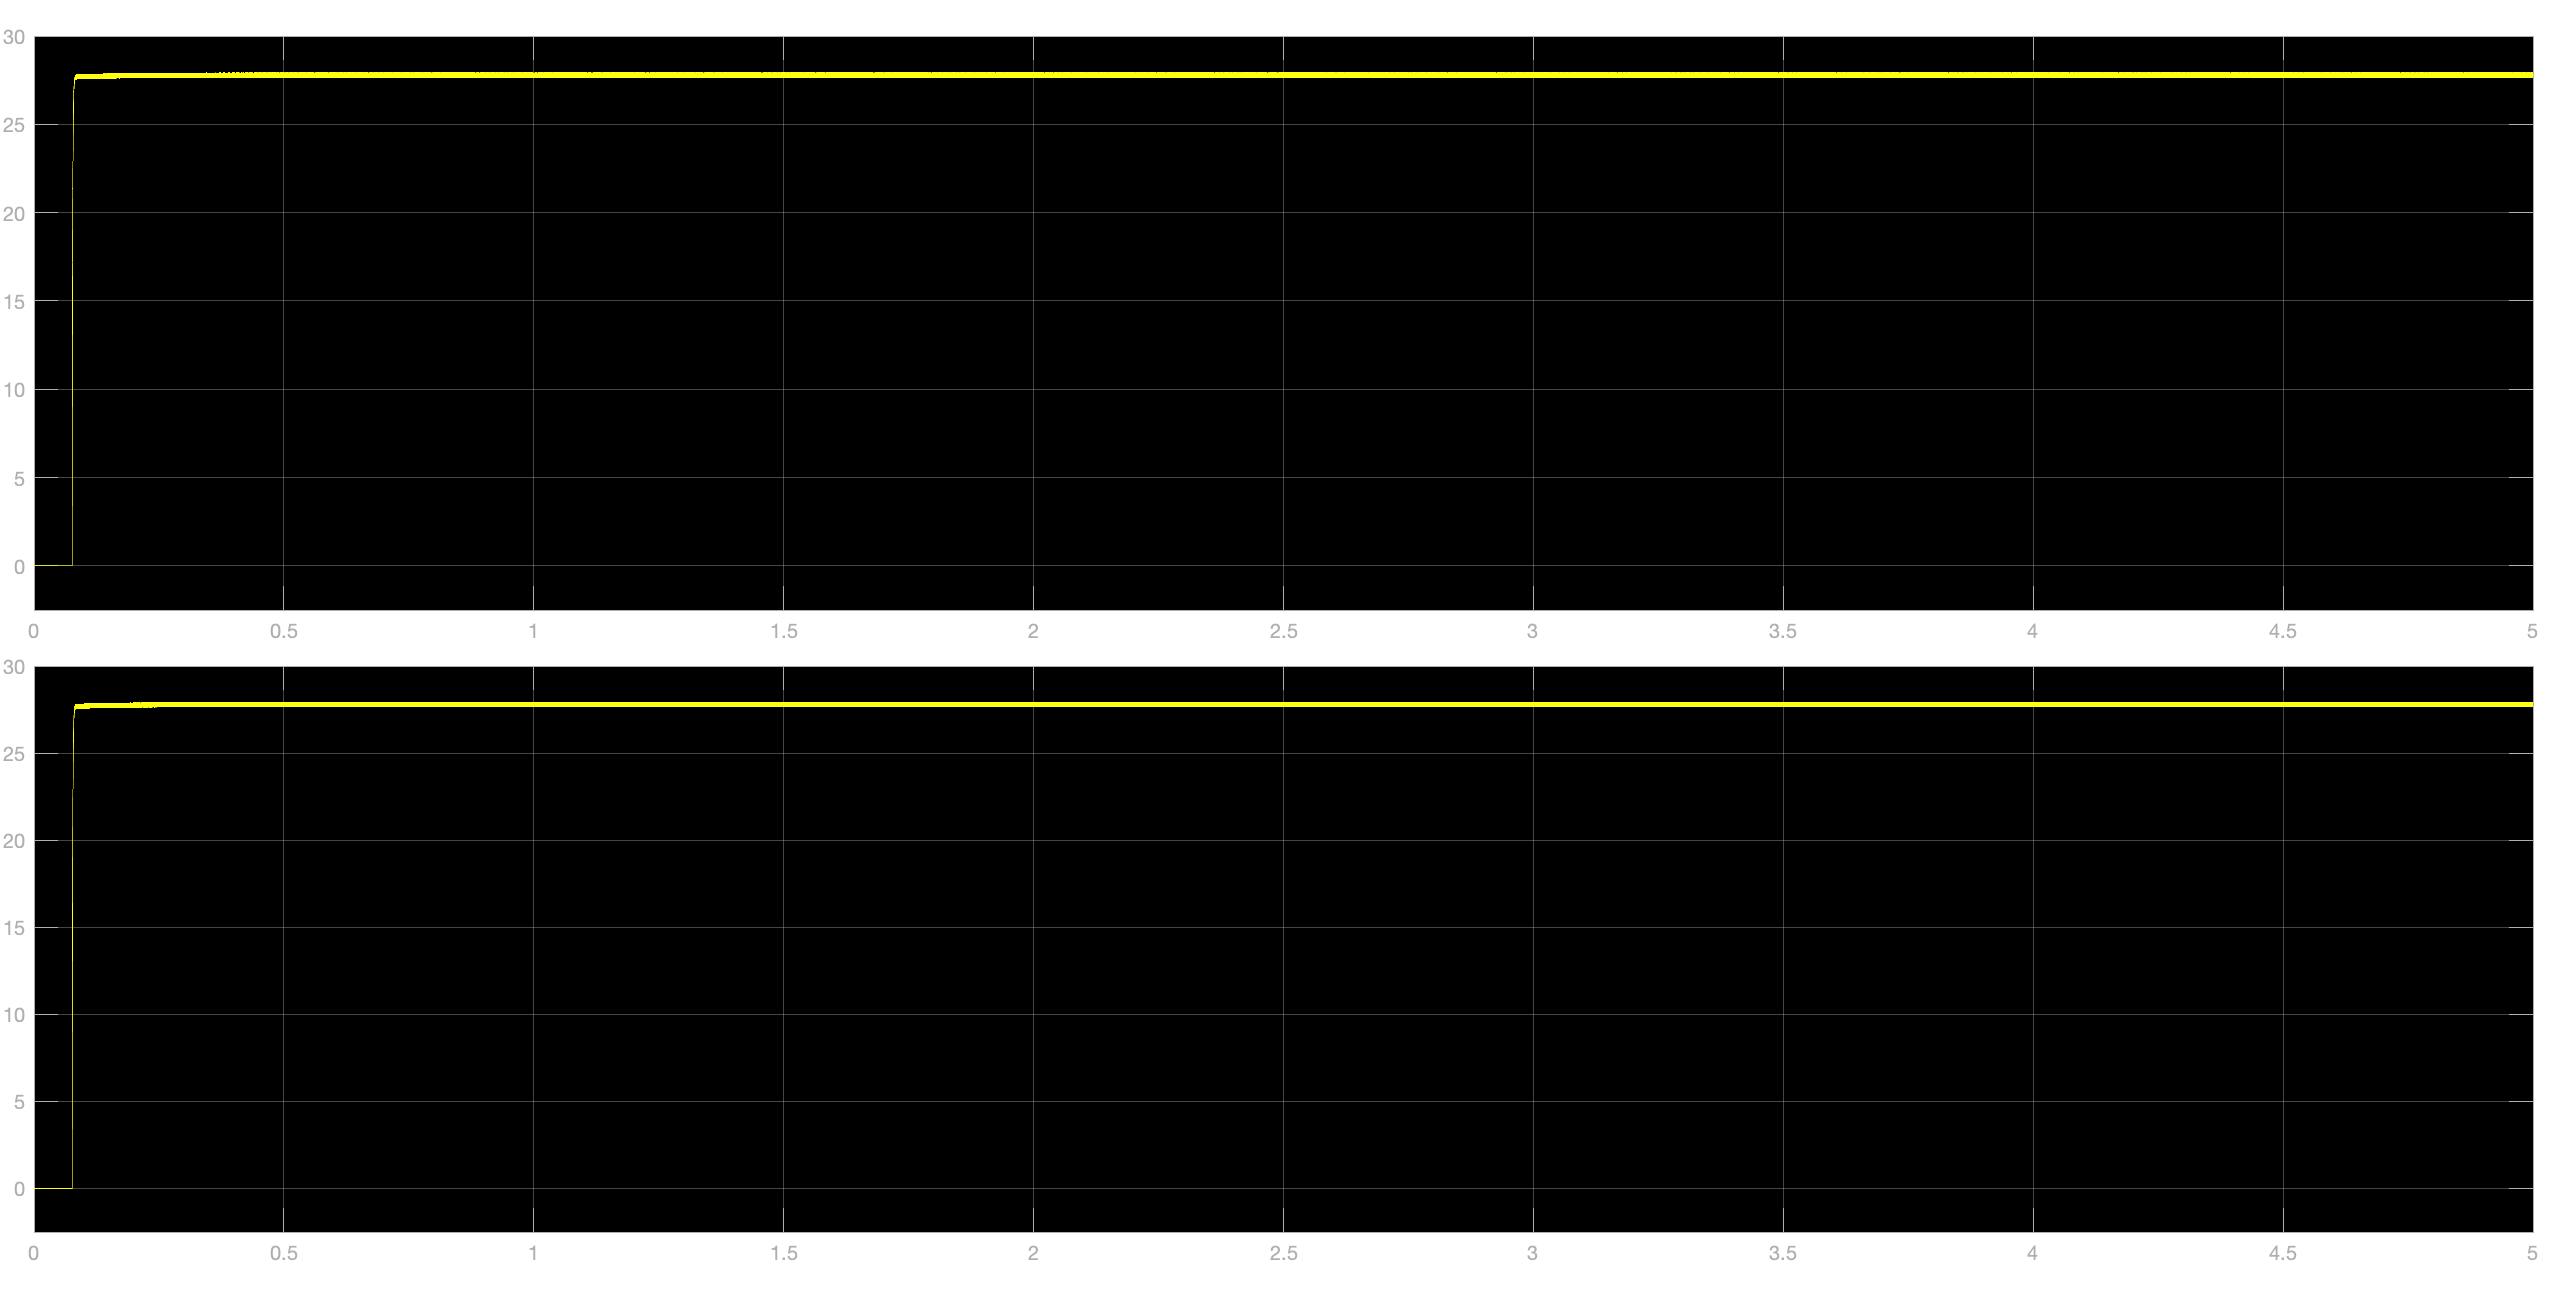
\includegraphics{gl_al_load2.png}}
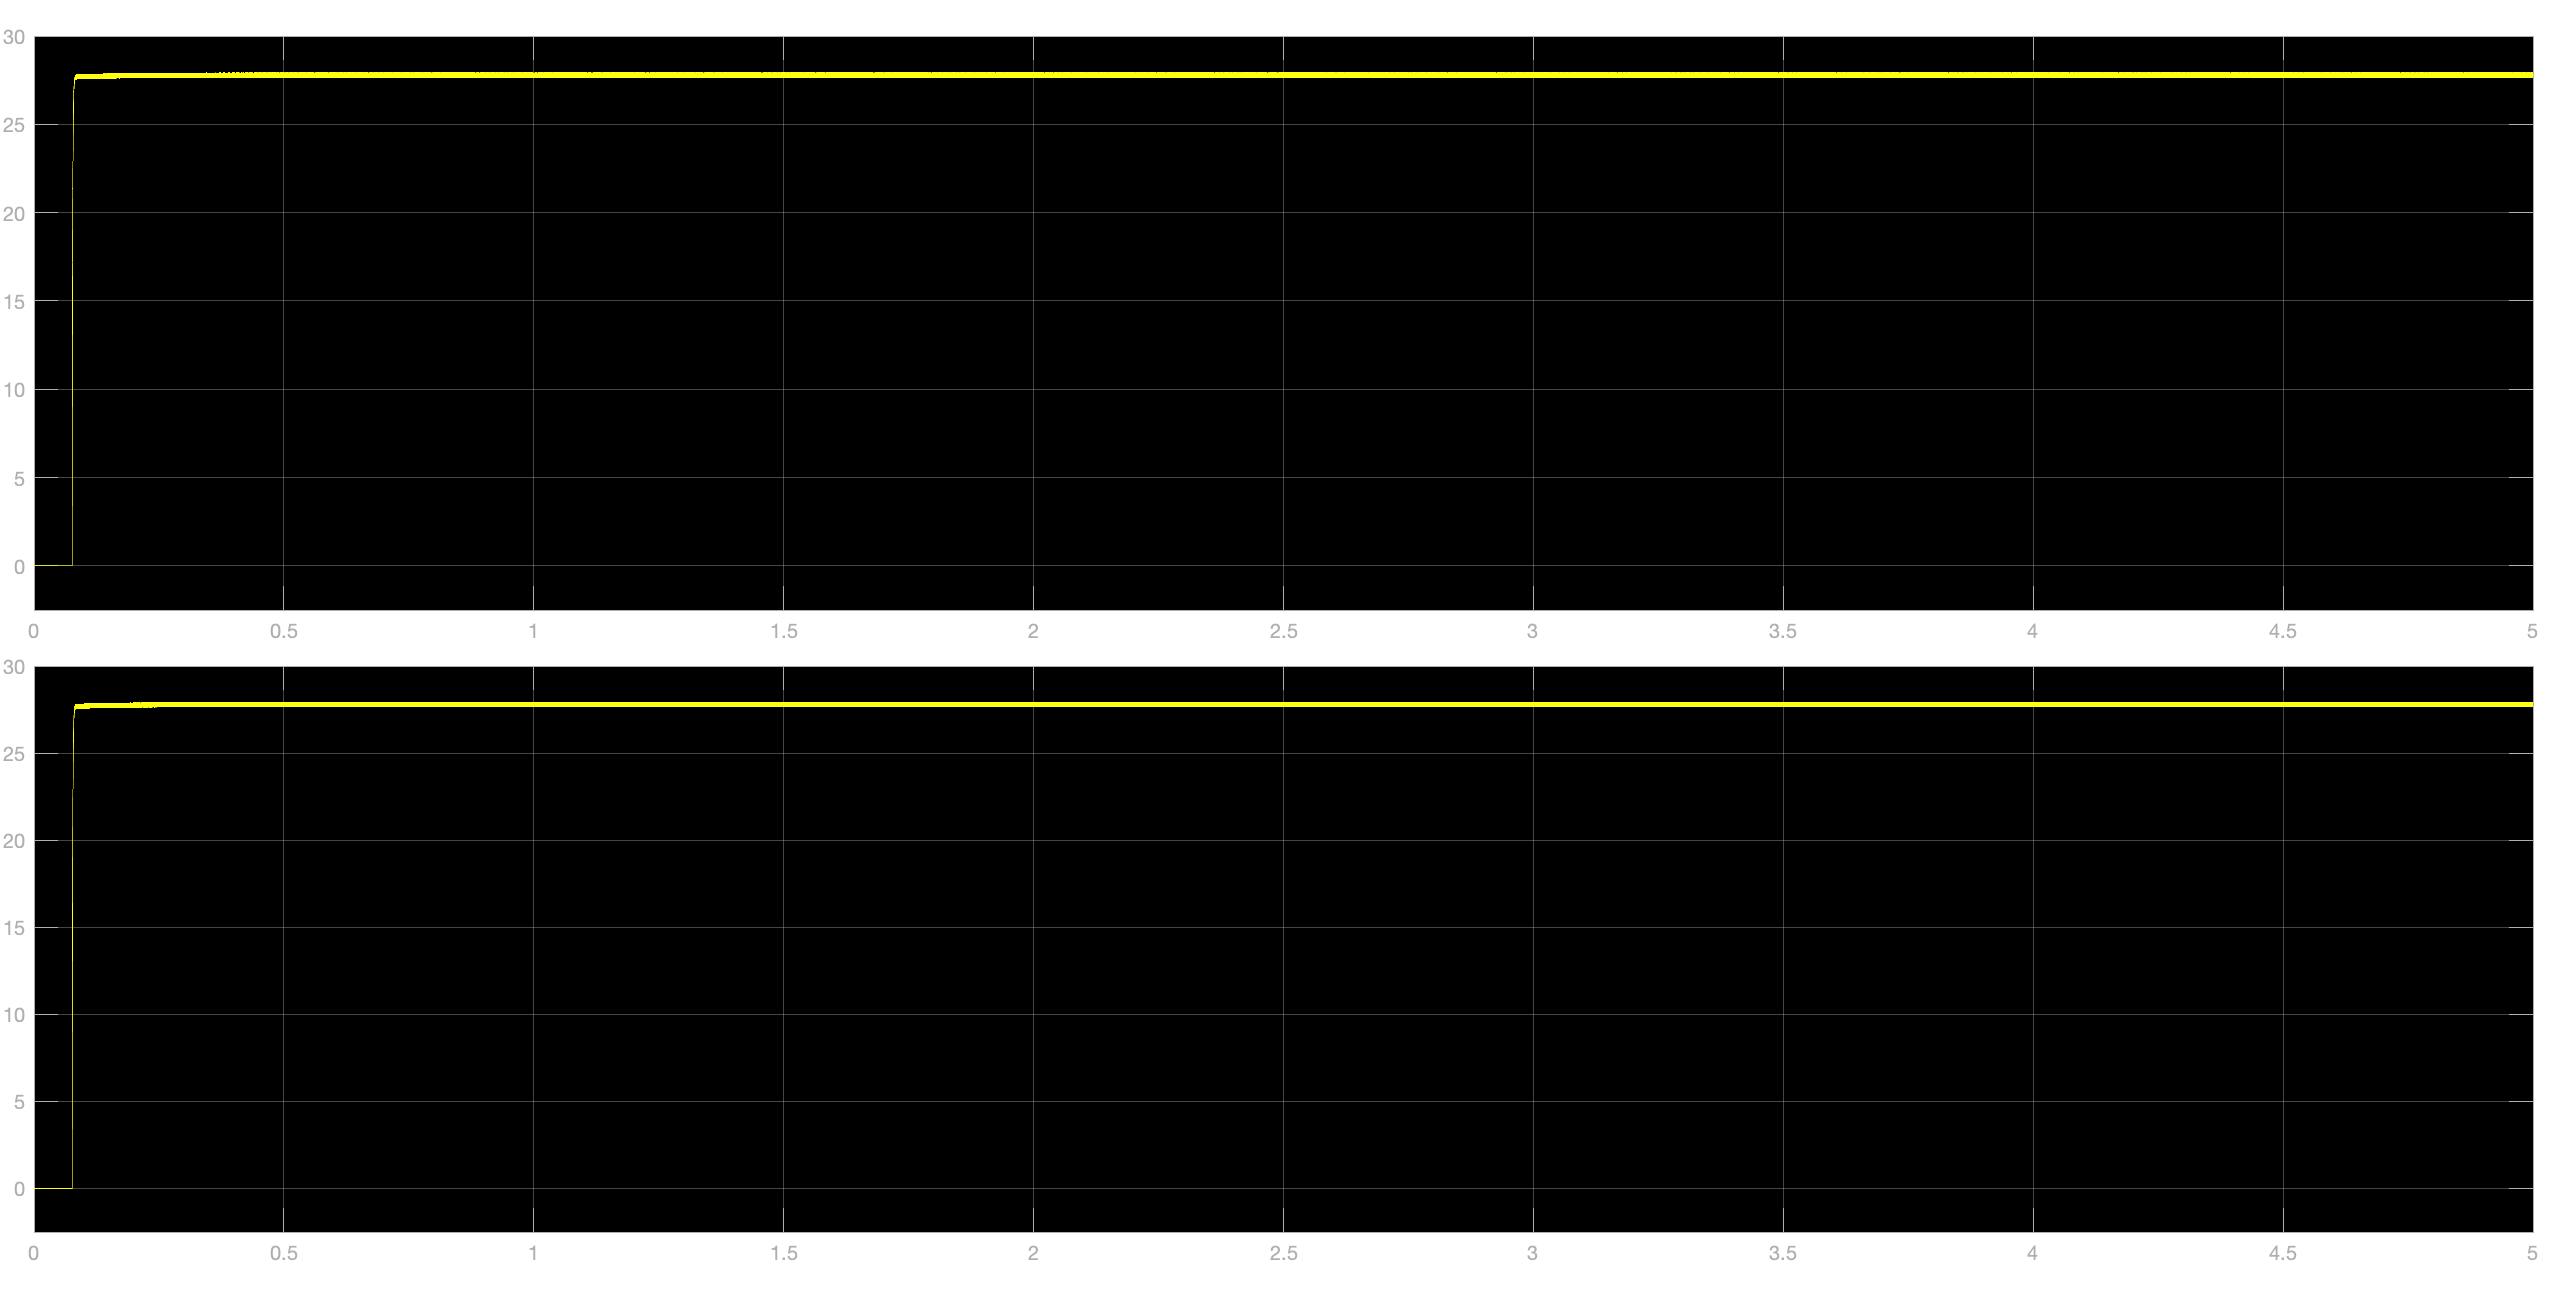
\includegraphics[trim= 0 0.255\imageheight{} 0 0, clip, width = 0.185\imageheight{}]{gl_al_load2.png}
\begin{center}
\small{Figure 2.6.2 Right DC Load Waveform}
\end{center}
\begin{center}
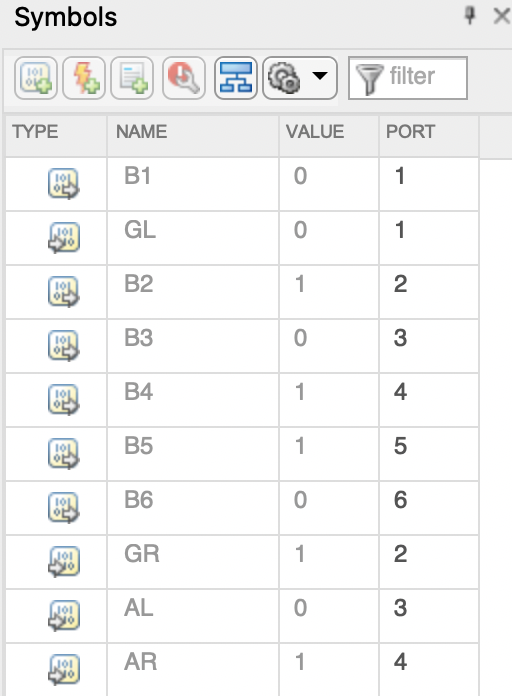
\includegraphics[width=4.5cm]{gl_al_signals.png}
\end{center}
\begin{center}
\small{Figure 2.6.3 BPCU Output Control Signals}
\end{center}
\begin{center}
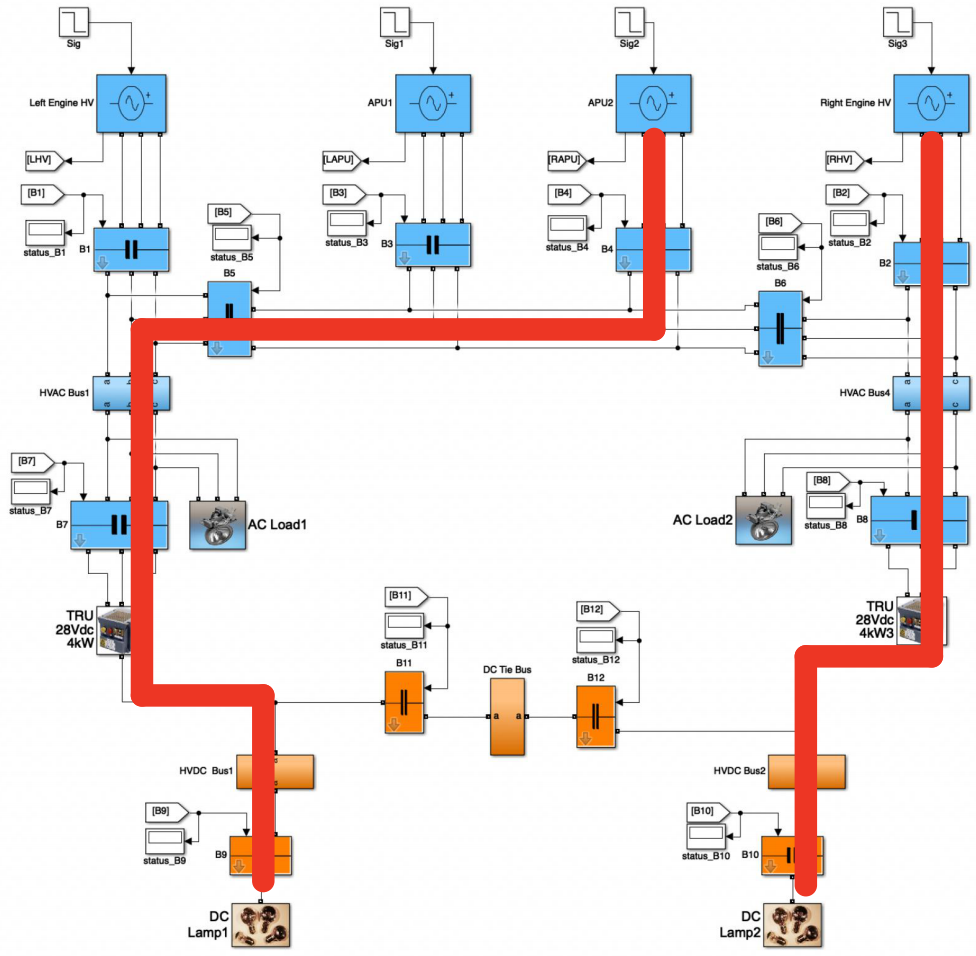
\includegraphics[width=14.5cm]{gl_al.png}
\end{center}
\begin{center}
\small{Figure 2.6.4 EPS Connection}
\end{center}
When GL and AL fail,  the leftmost available power supply AR empowers the left AC bus based on system guarantee G7. Only one APU, AR, is used based on system guarantee G4.
\pagebreak

\subsection{Case 6: GR, GL Not Working}
\settowidth{\imageheight}{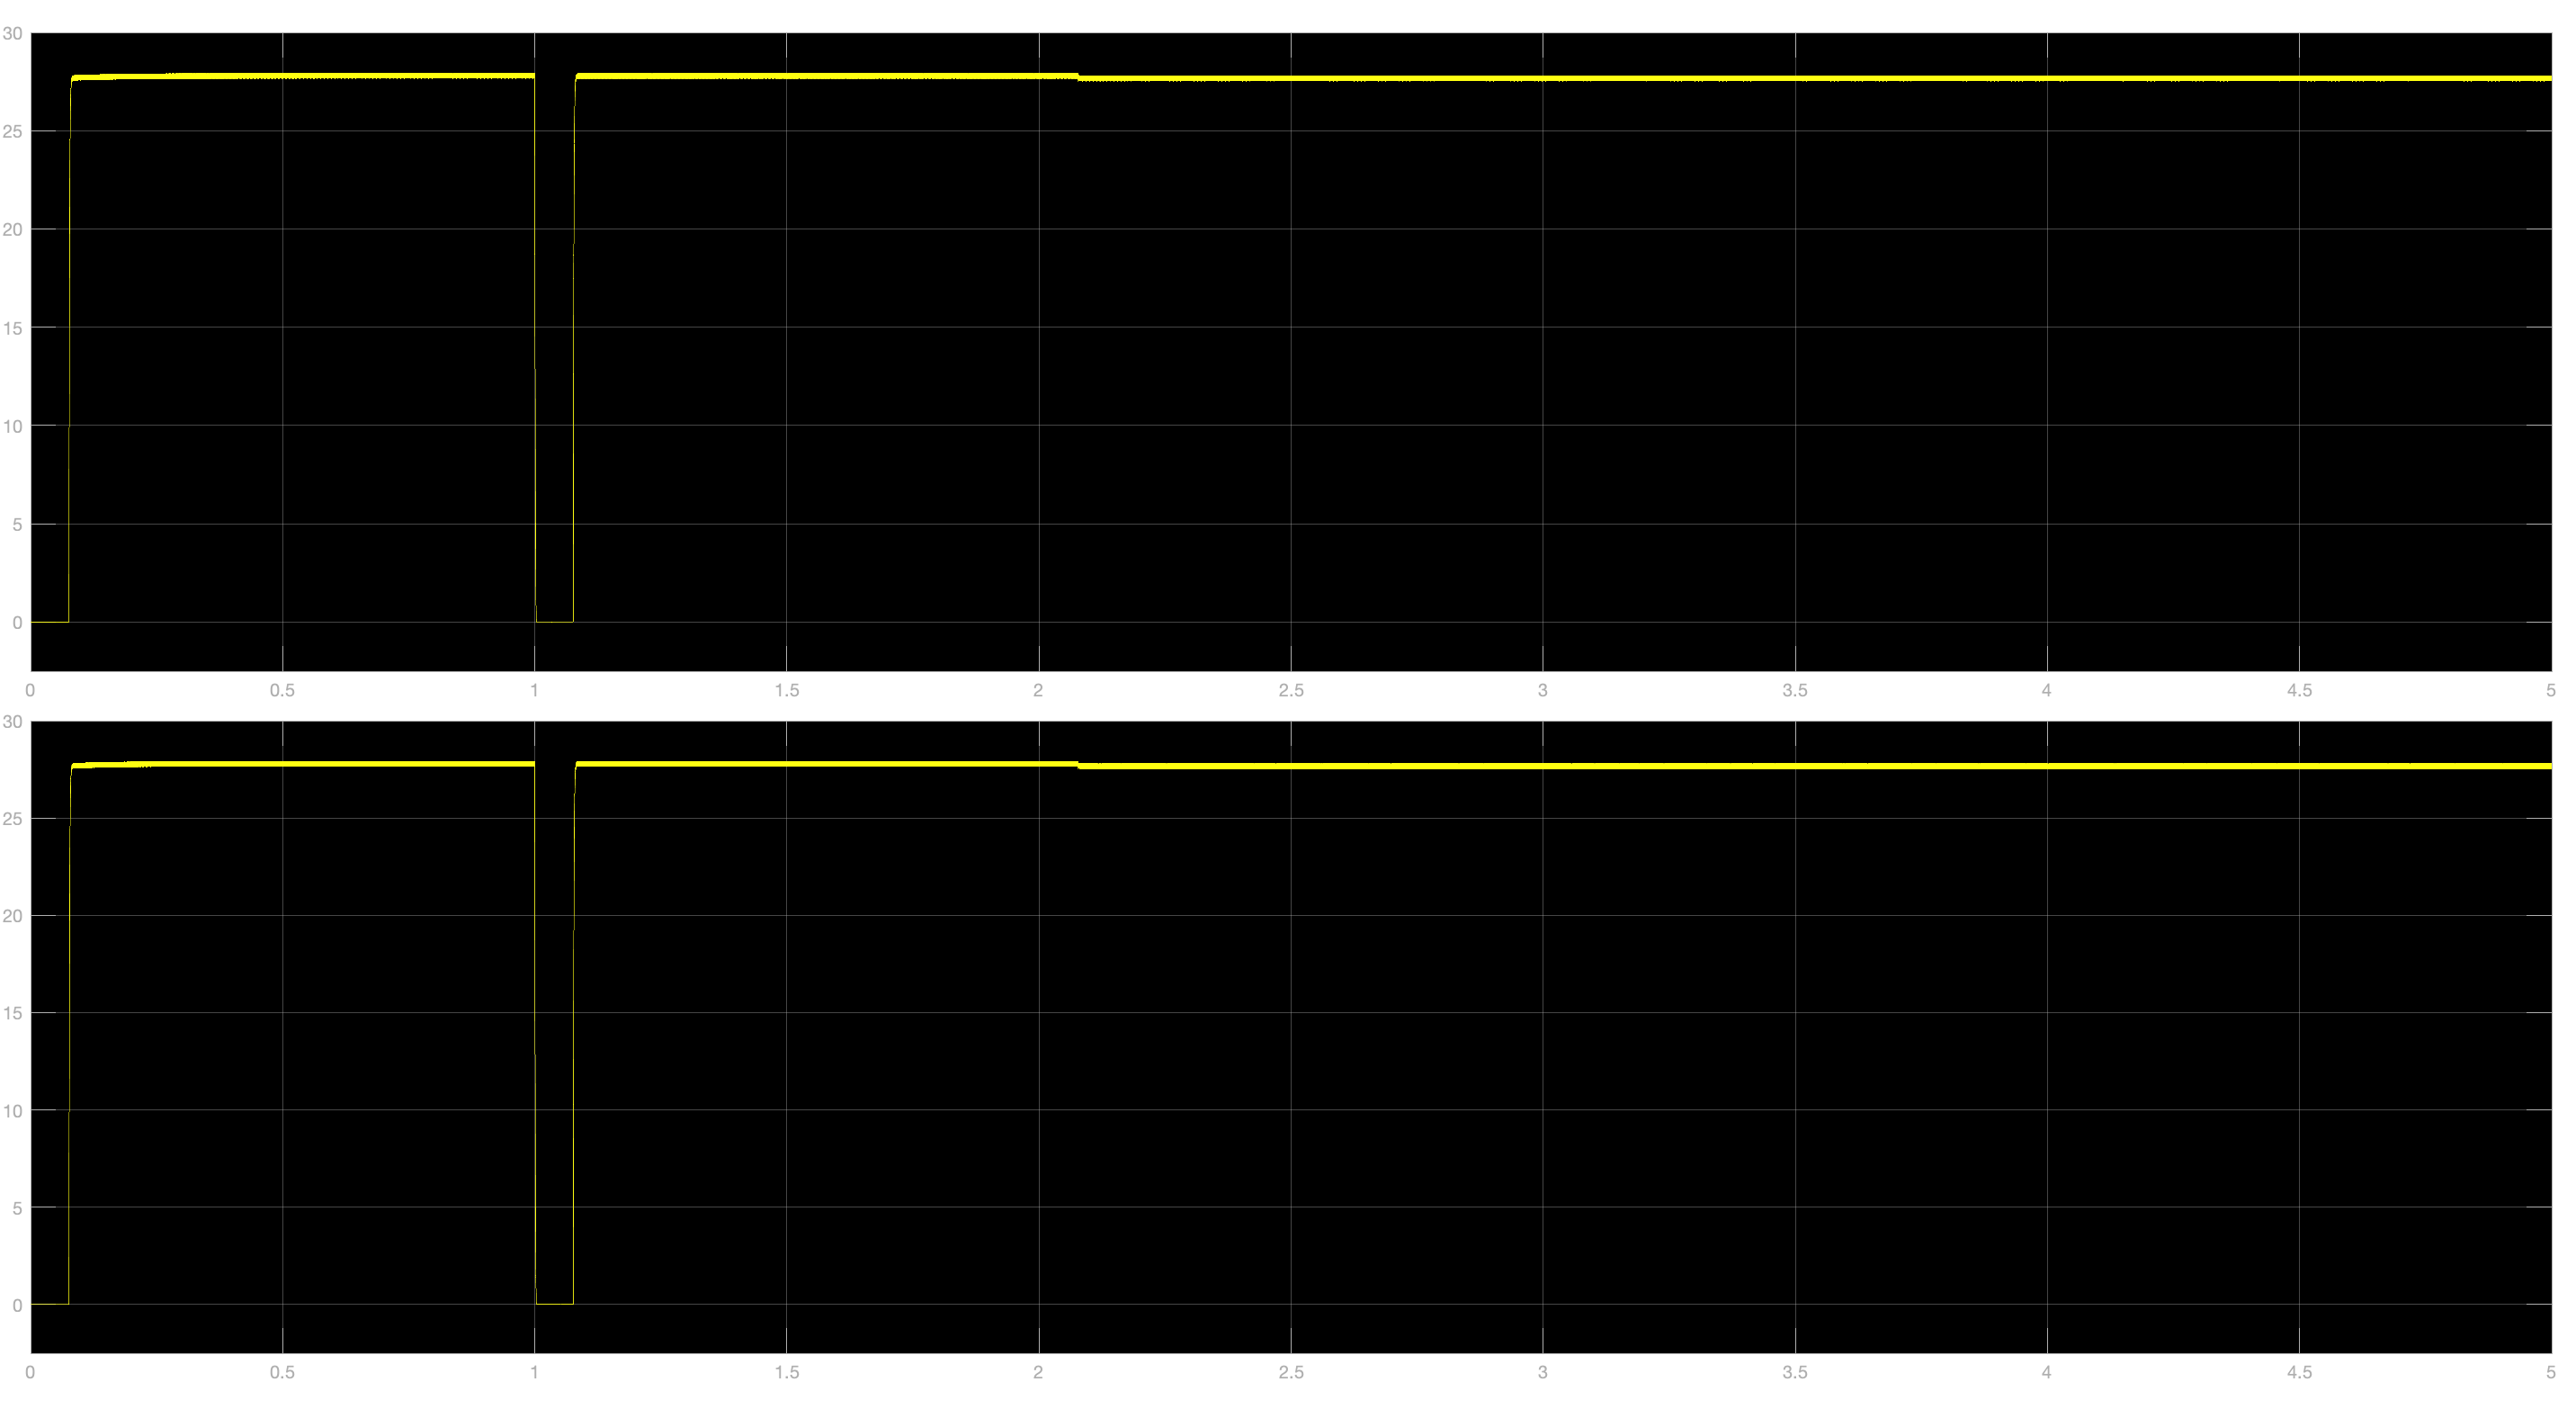
\includegraphics{gl_gr_load1.png}}
\begin{center}
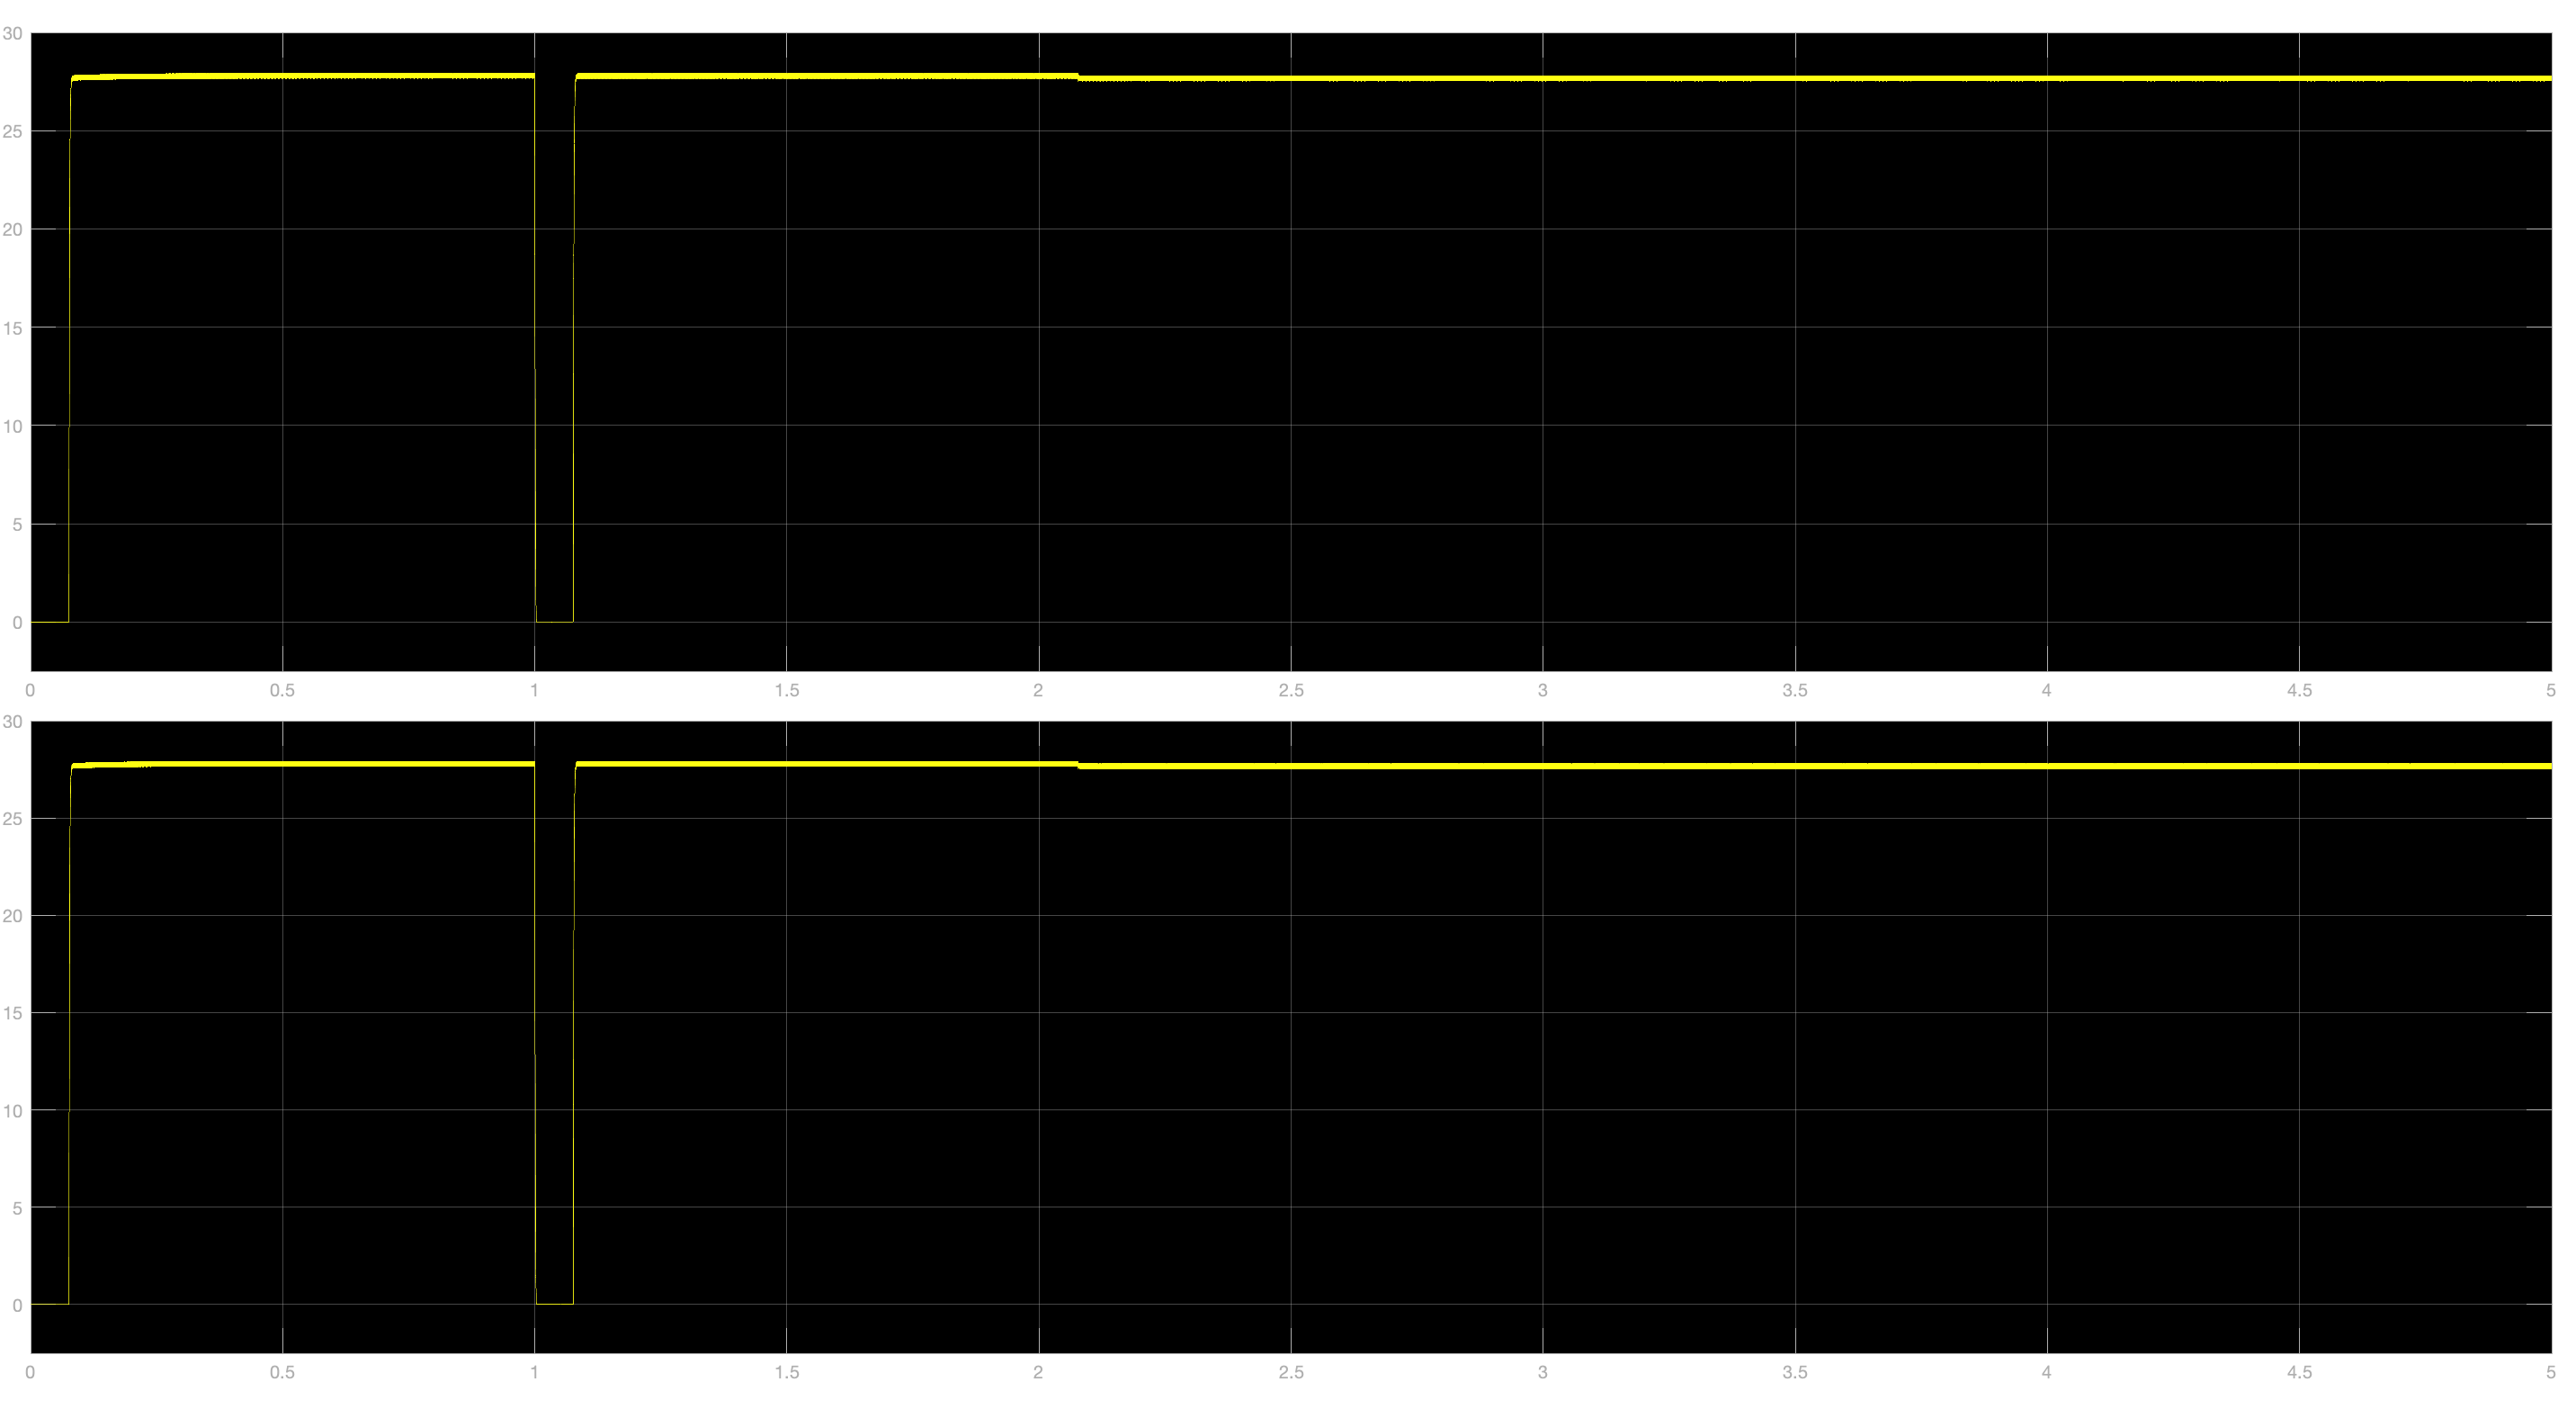
\includegraphics[trim= 0 0.28\imageheight{} 0 0, clip, width = 0.165\imageheight{}]{gl_gr_load1.png}
\end{center}
\begin{center}
\small{Figure 2.7.1 Left DC Load Waveform}
\end{center}
\settowidth{\imageheight}{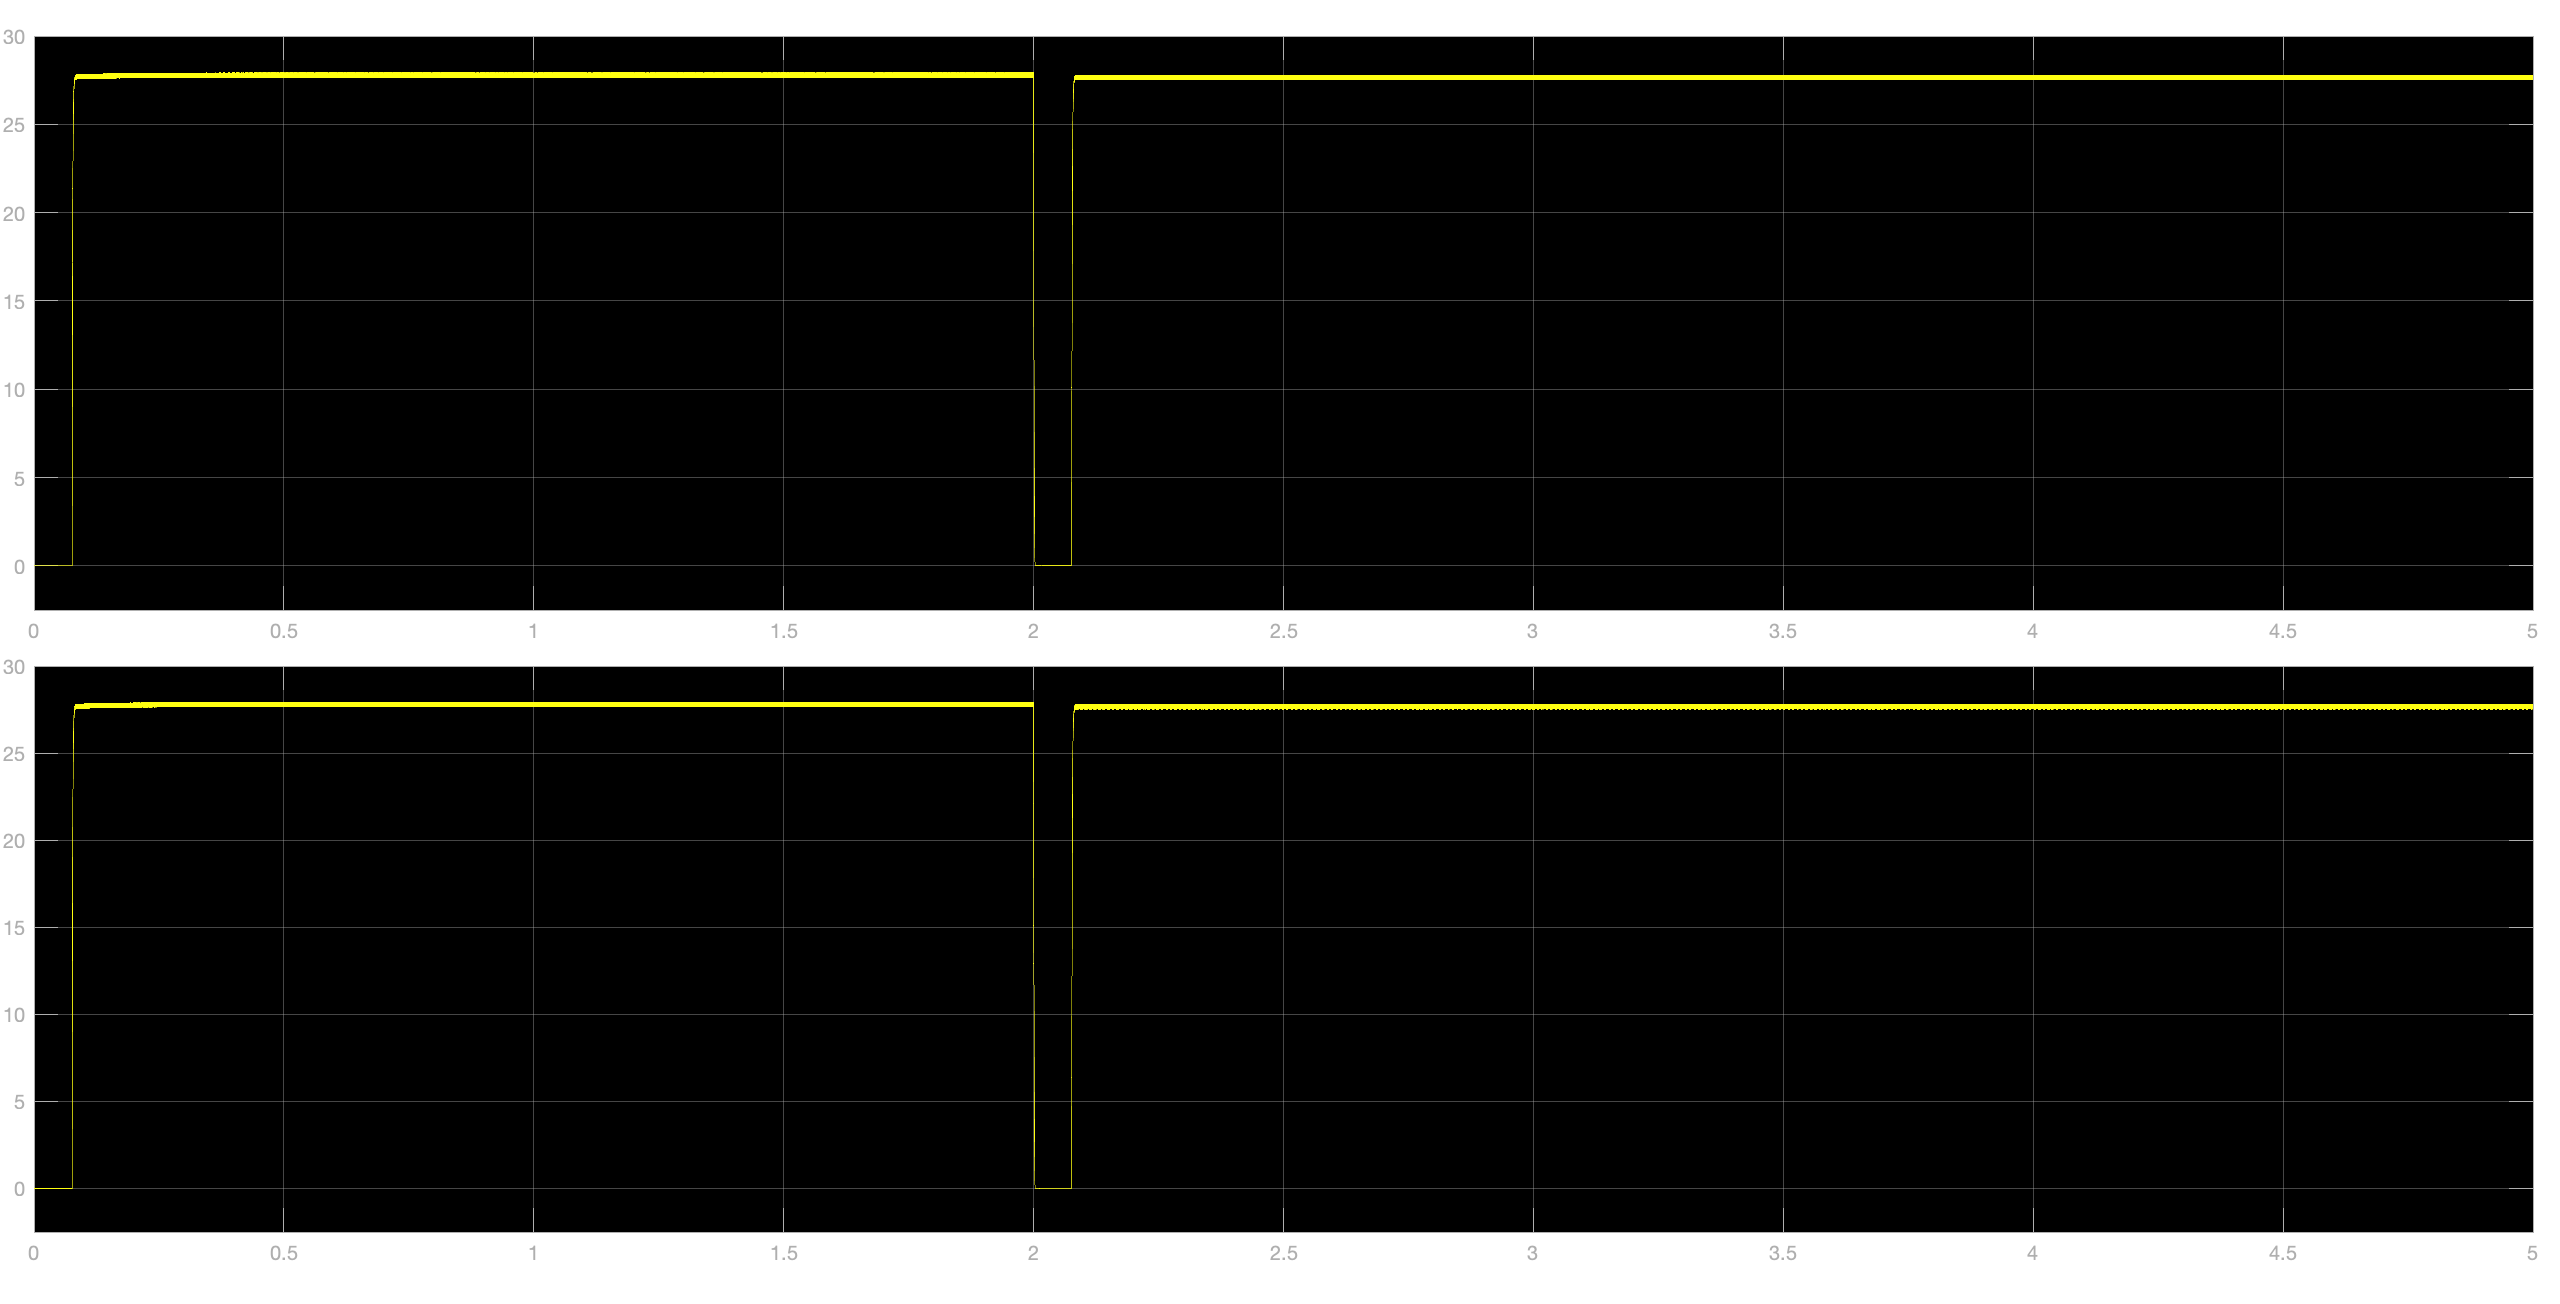
\includegraphics{gl_gr_load2.png}}
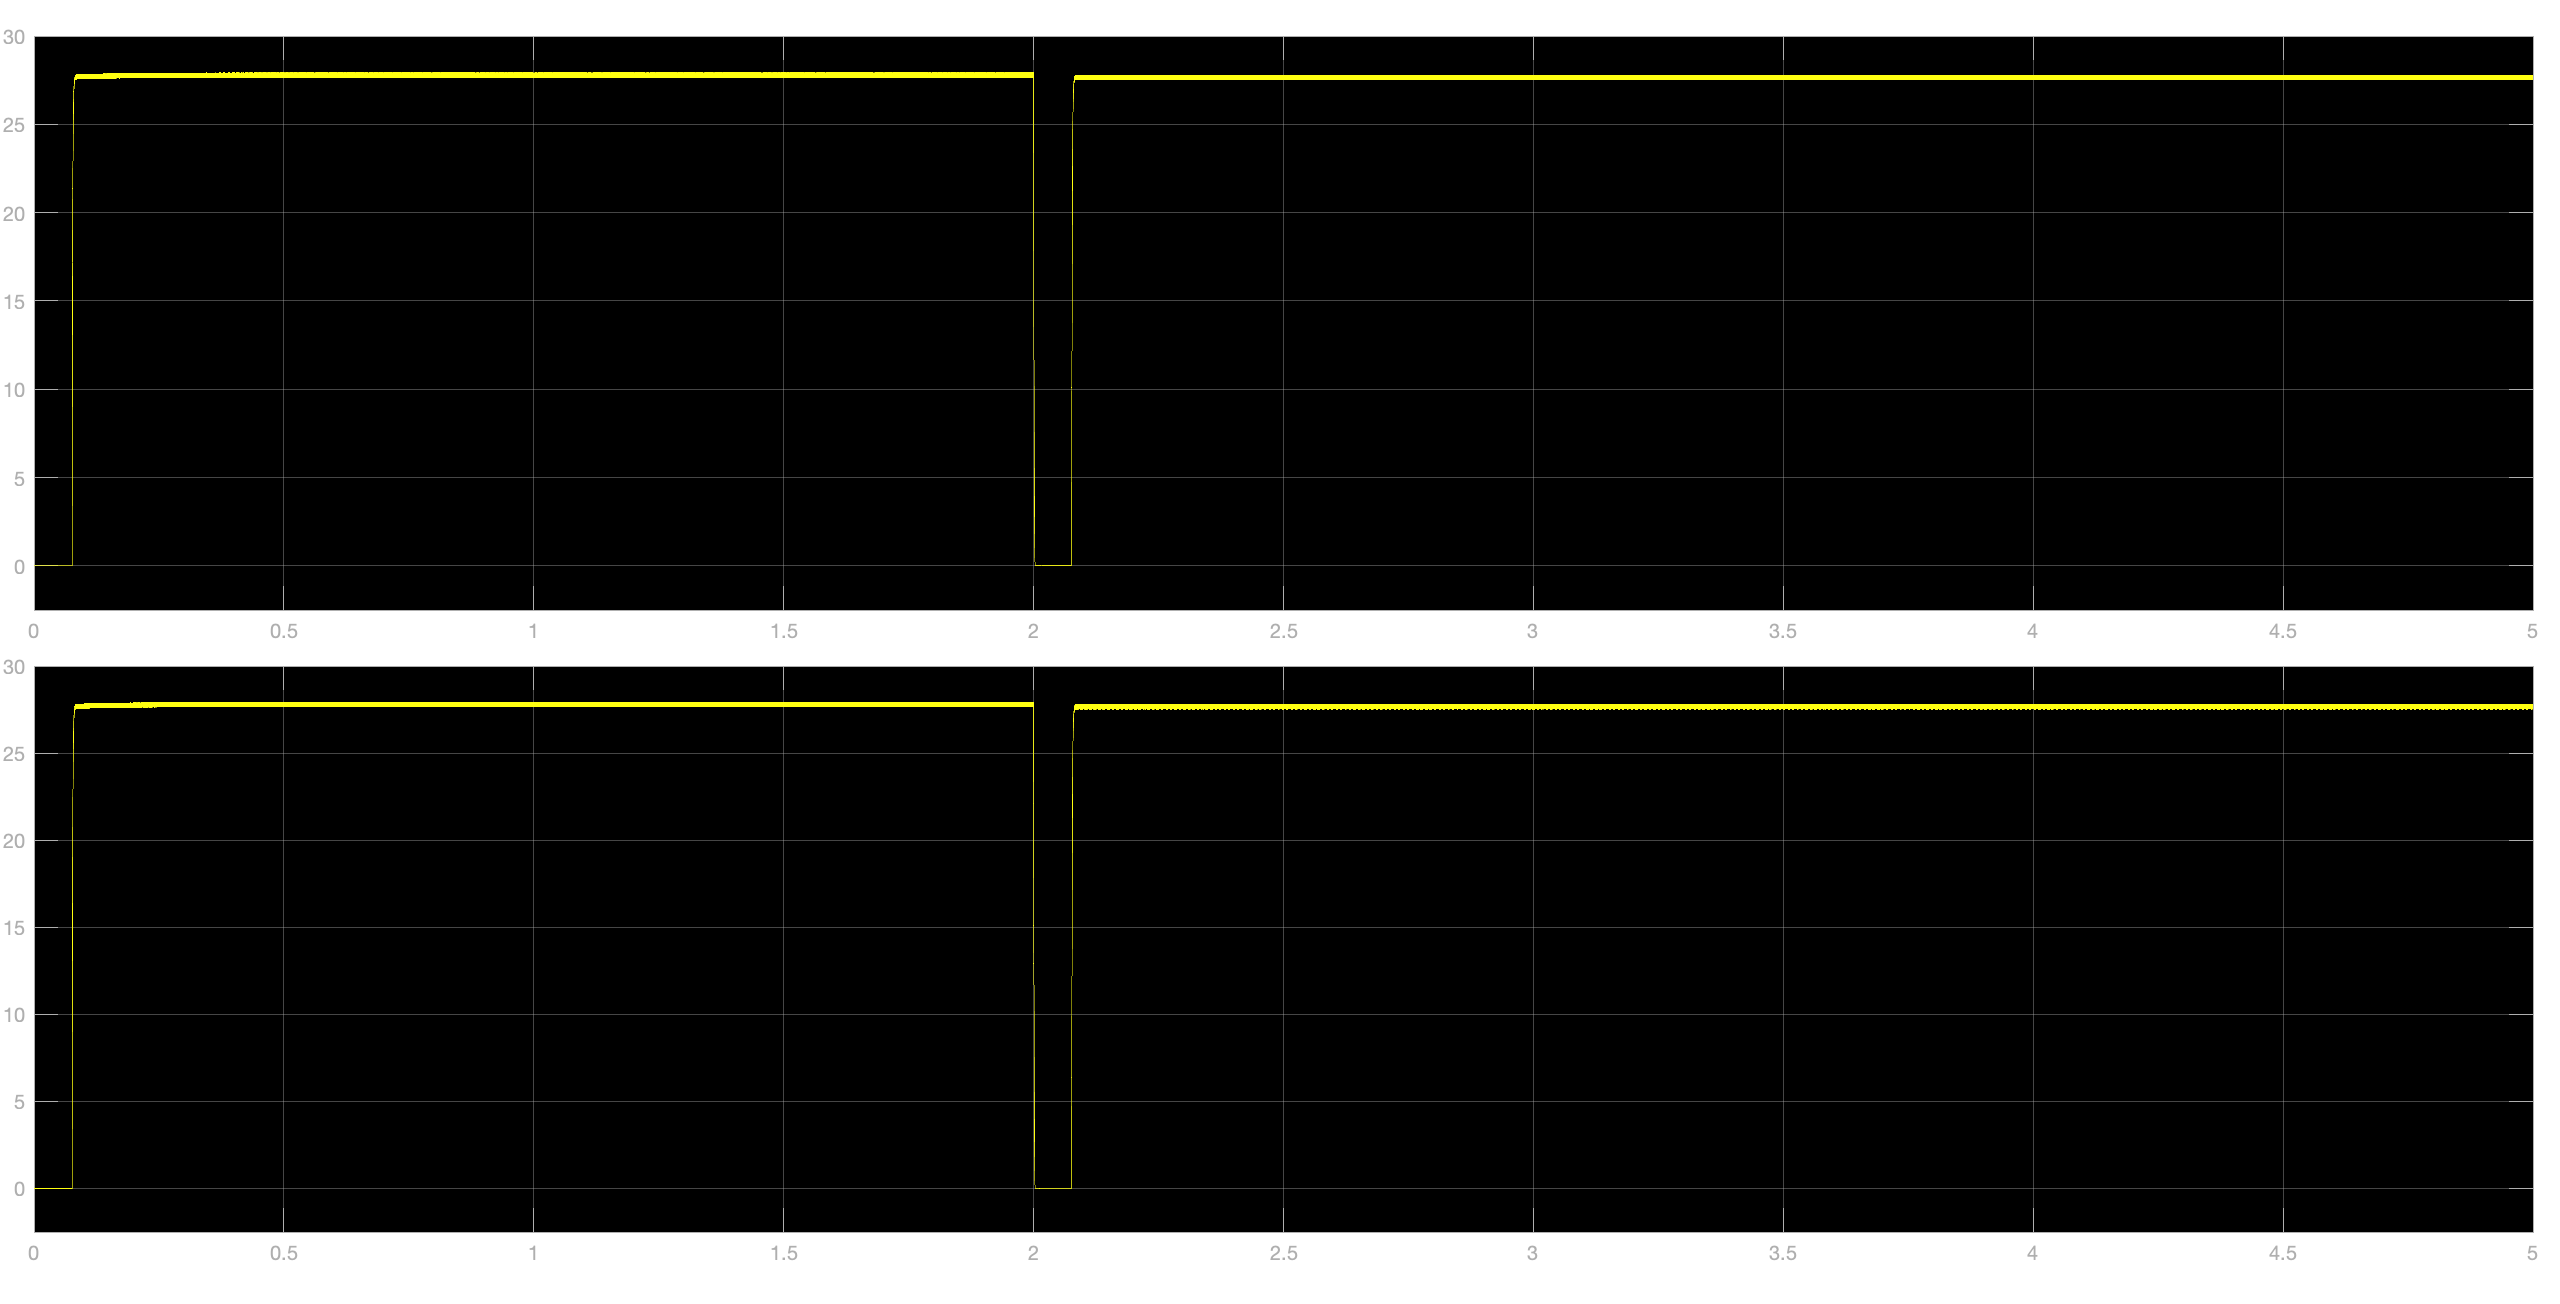
\includegraphics[trim= 0 0.255\imageheight{} 0 0, clip, width = 0.185\imageheight{}]{gl_gr_load2.png}
\begin{center}
\small{Figure 2.7.2 Right DC Load Waveform}
\end{center}
\begin{center}
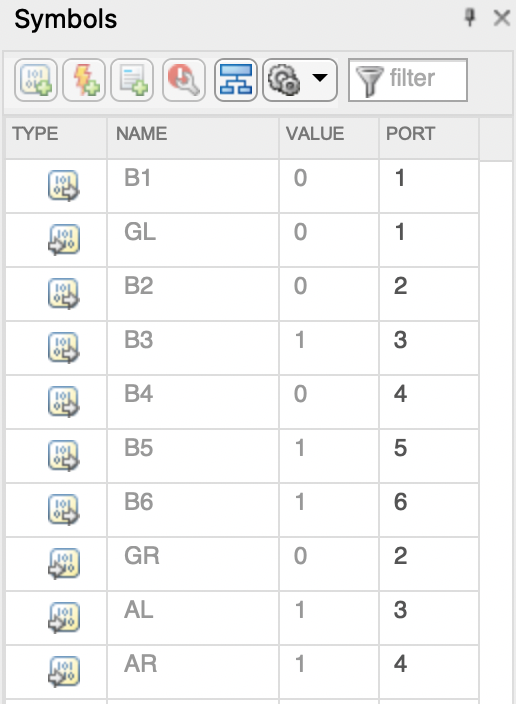
\includegraphics[width=4.5cm]{gl_gr_signals.png}
\end{center}
\begin{center}
\small{Figure 2.7.3 BPCU Output Control Signals}
\end{center}
\begin{center}
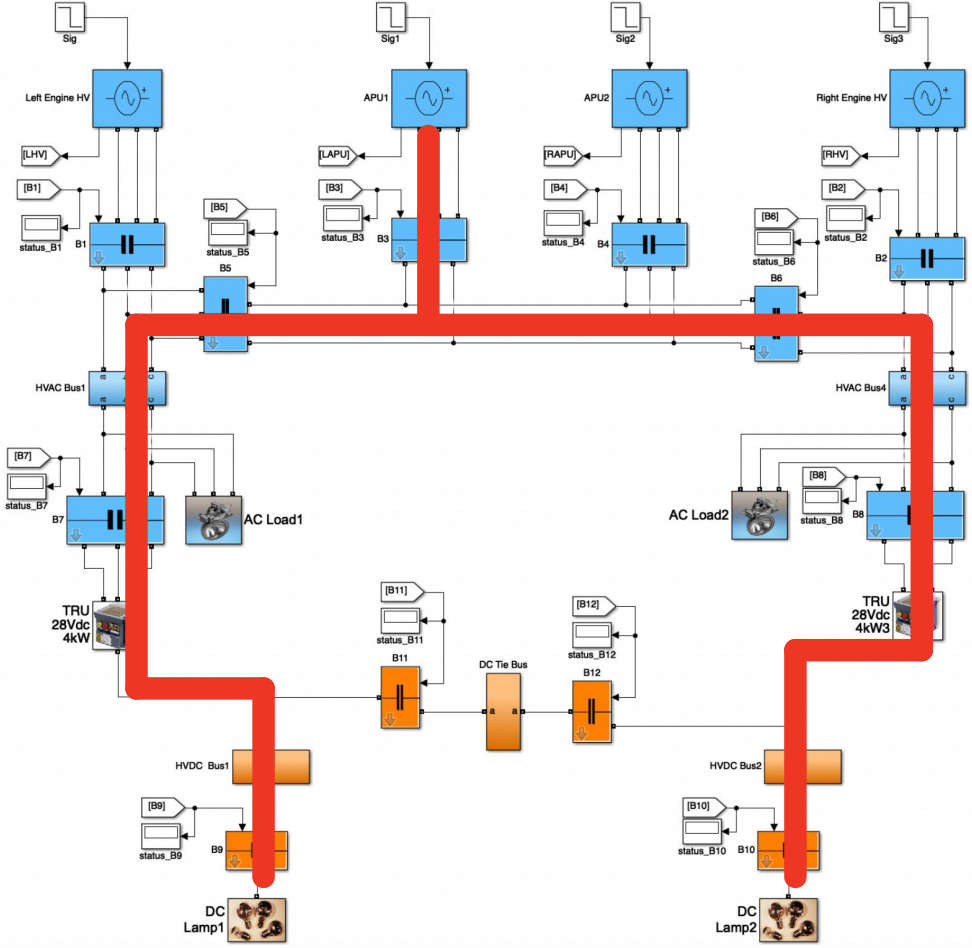
\includegraphics[width=14.5cm]{gl_gr.png}
\end{center}
\begin{center}
\small{Figure 2.7.4 EPS Connection}
\end{center}
When both GR and GL fail, only one APU, AL,  is inserted into the network and empowers both AC buses based on system guarantee G4, G7, and G8.
\pagebreak

\subsection{Case 7: GR, GL, AR Not Working}
\settowidth{\imageheight}{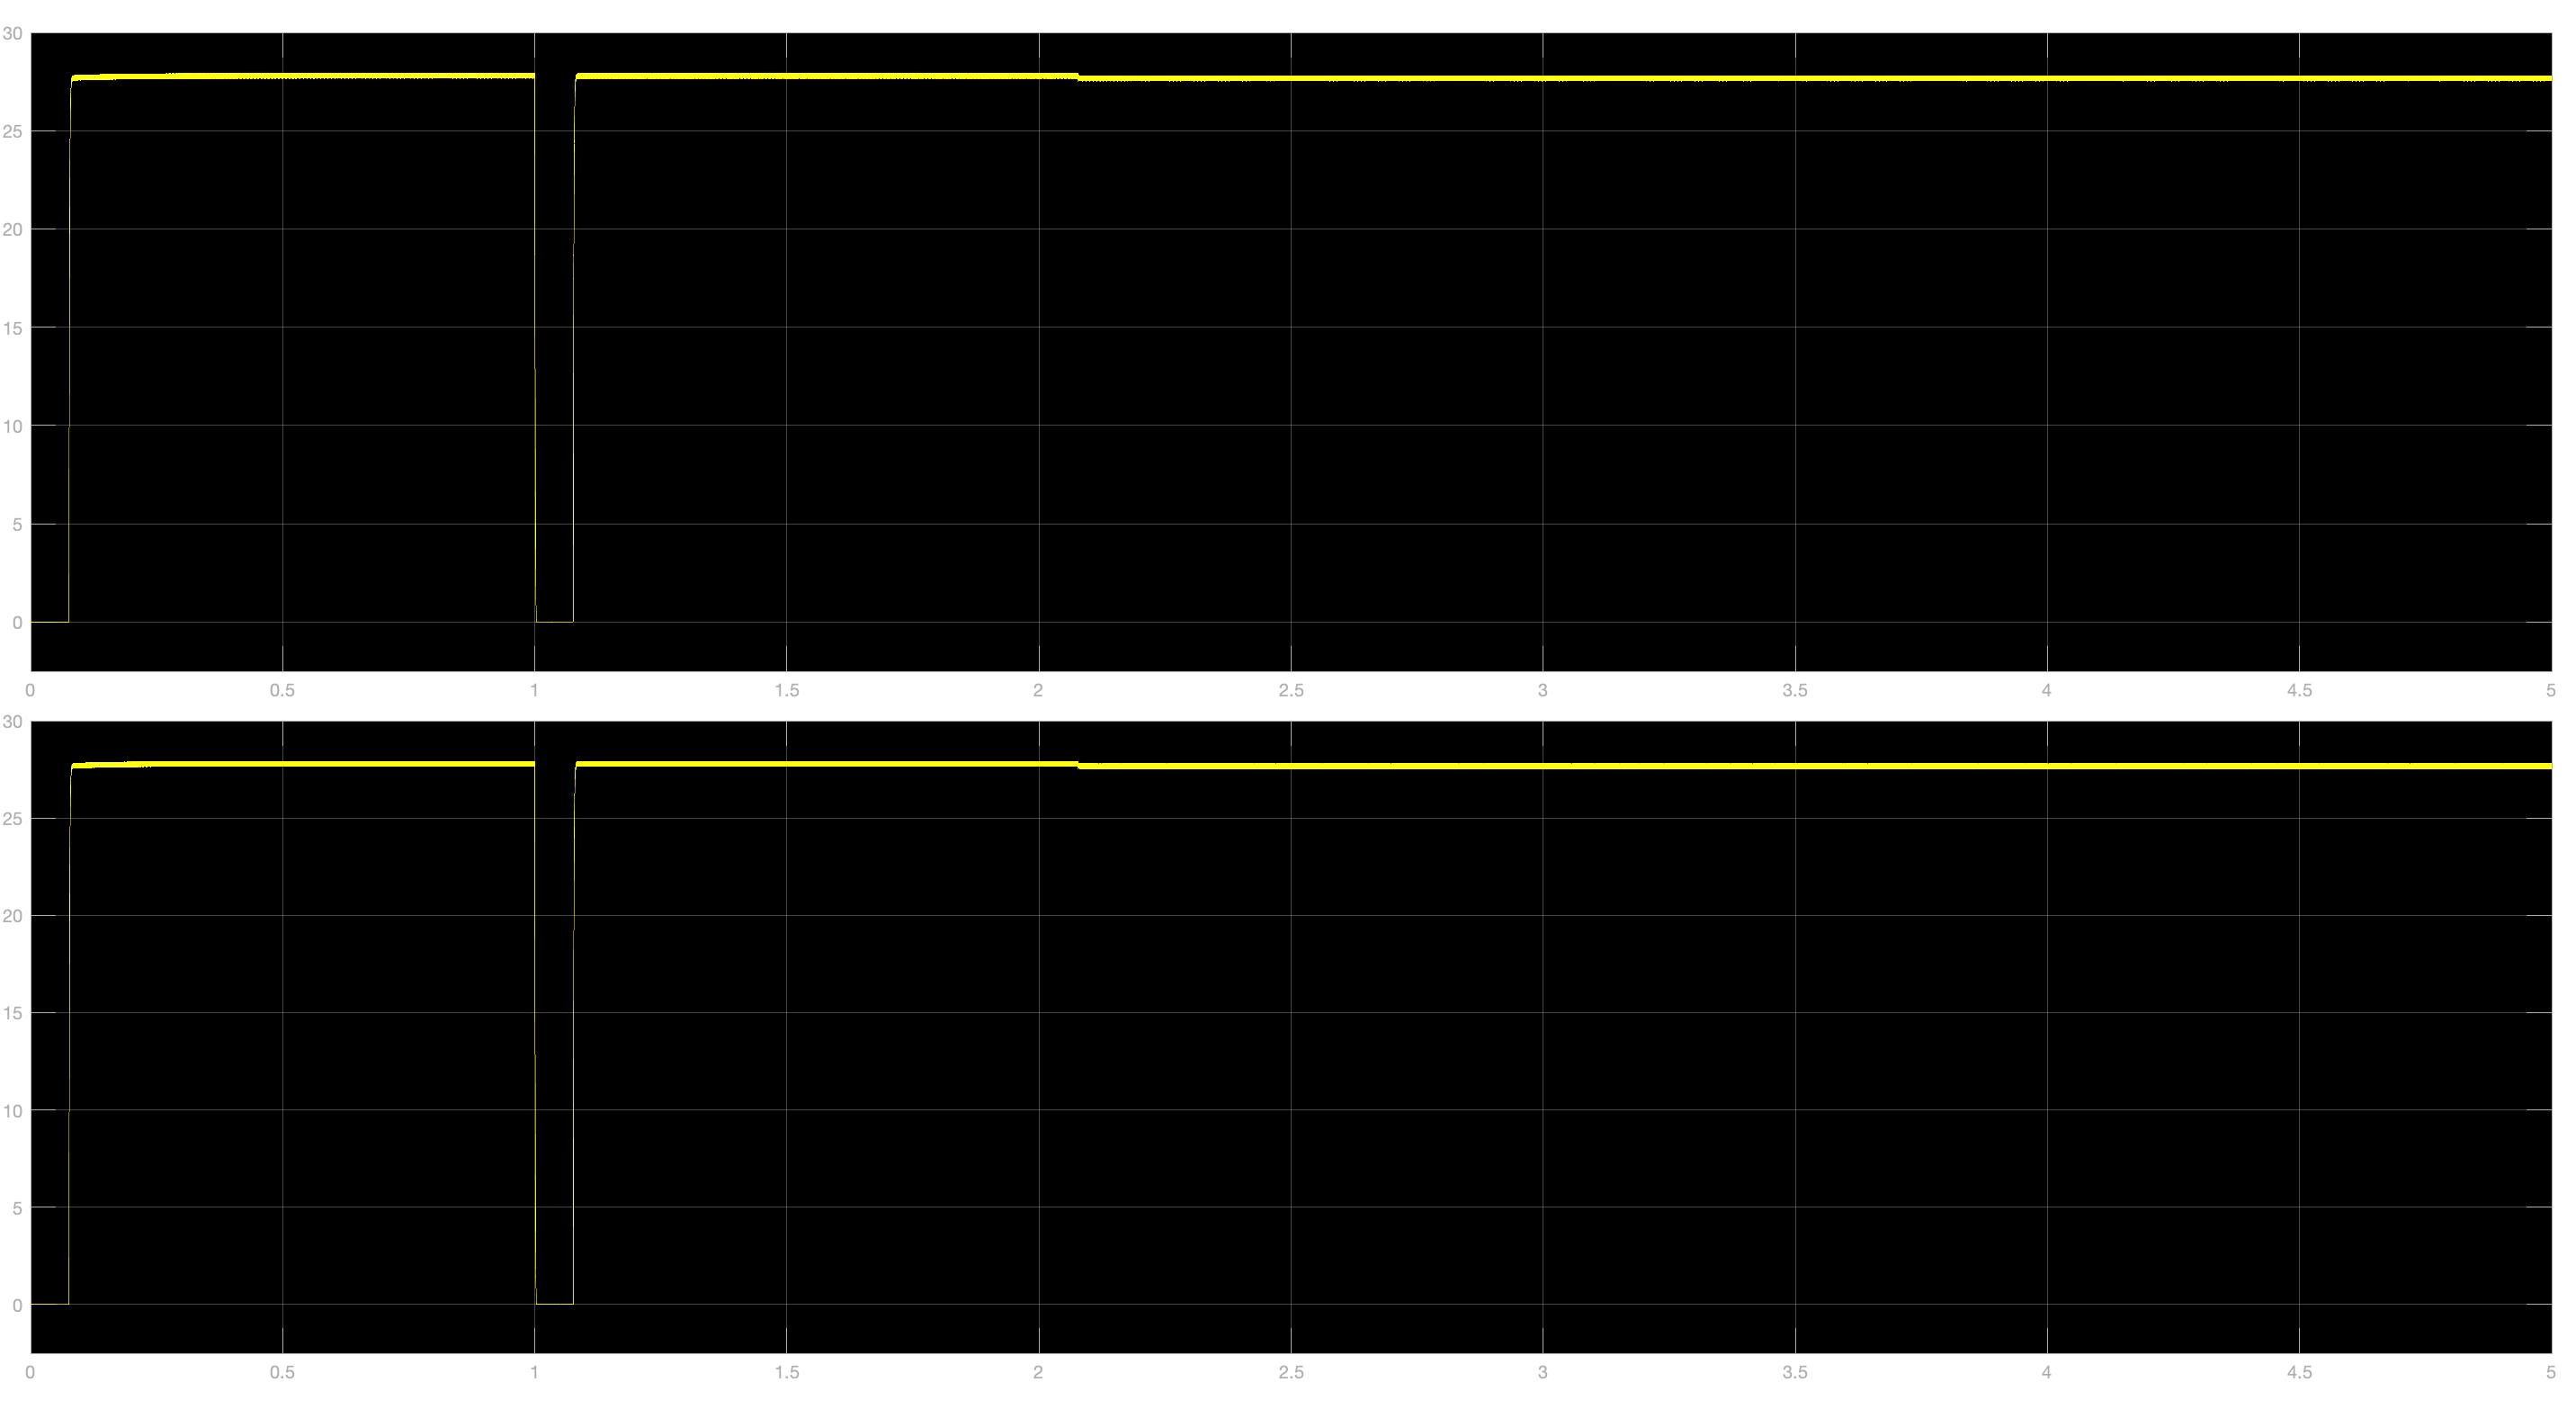
\includegraphics{gl_gr_ar_load1.png}}
\begin{center}
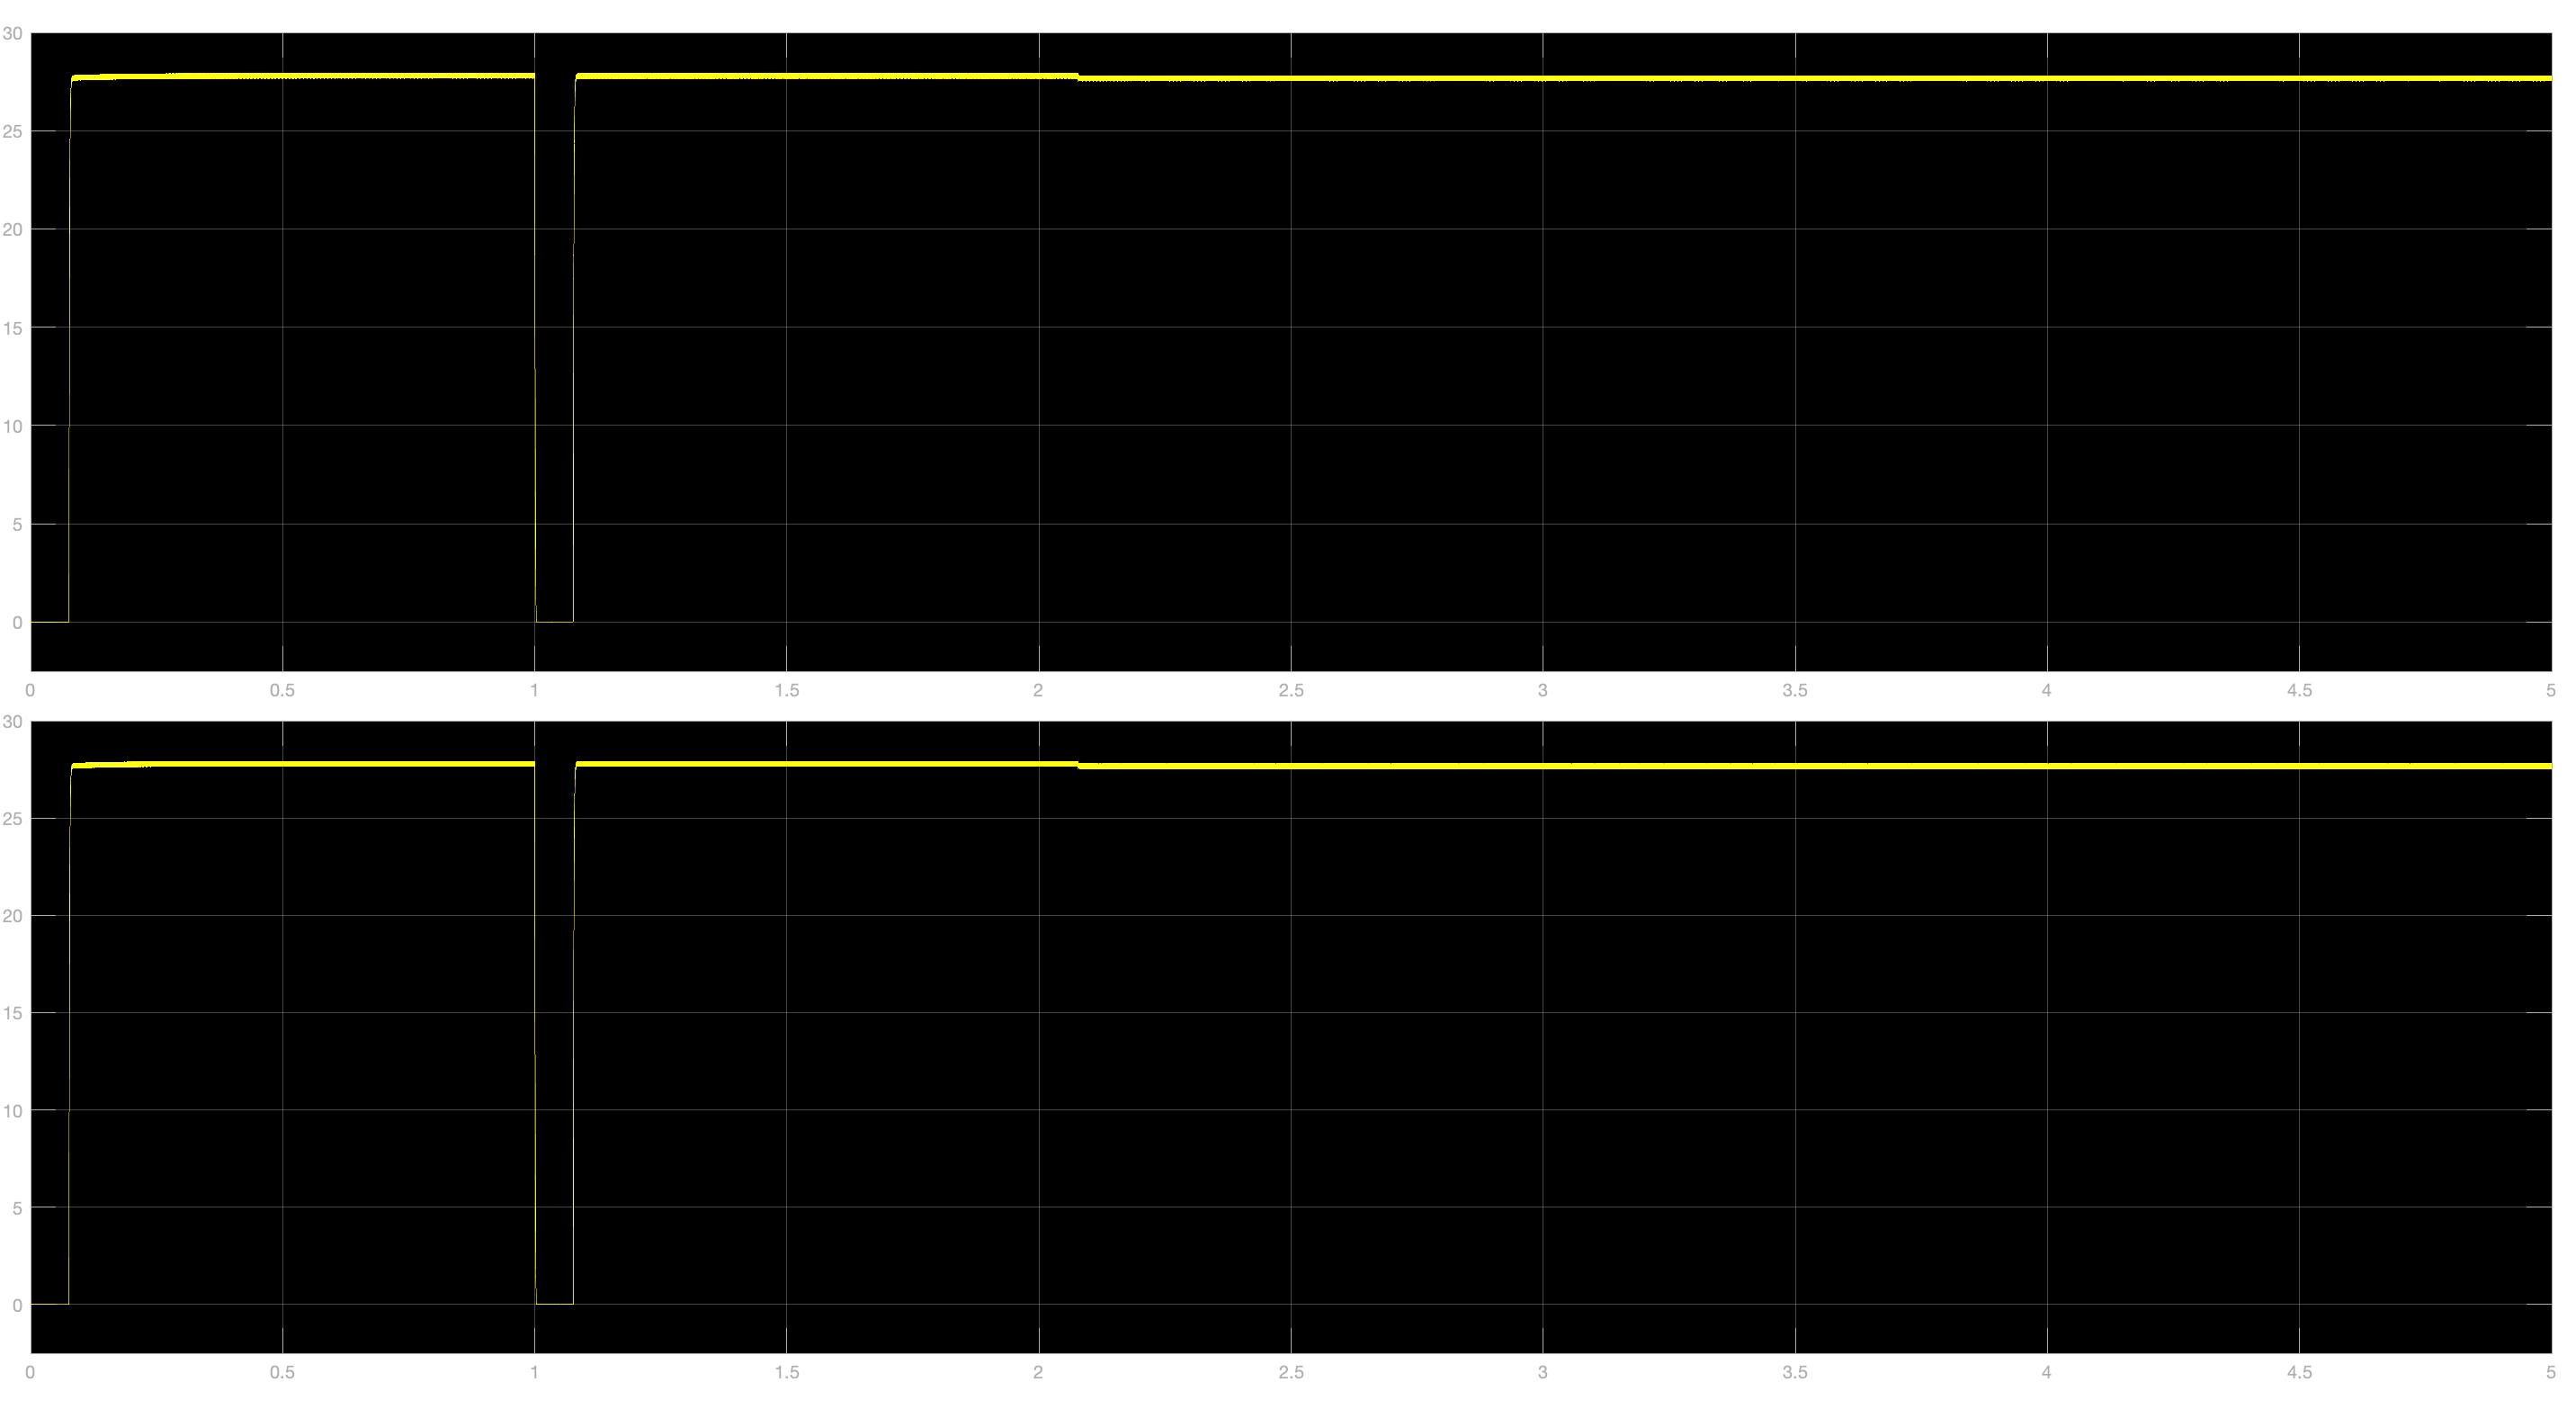
\includegraphics[trim= 0 0.28\imageheight{} 0 0, clip, width = 0.165\imageheight{}]{gl_gr_ar_load1.png}
\end{center}
\begin{center}
\small{Figure 2.8.1 Left DC Load Waveform}
\end{center}
\settowidth{\imageheight}{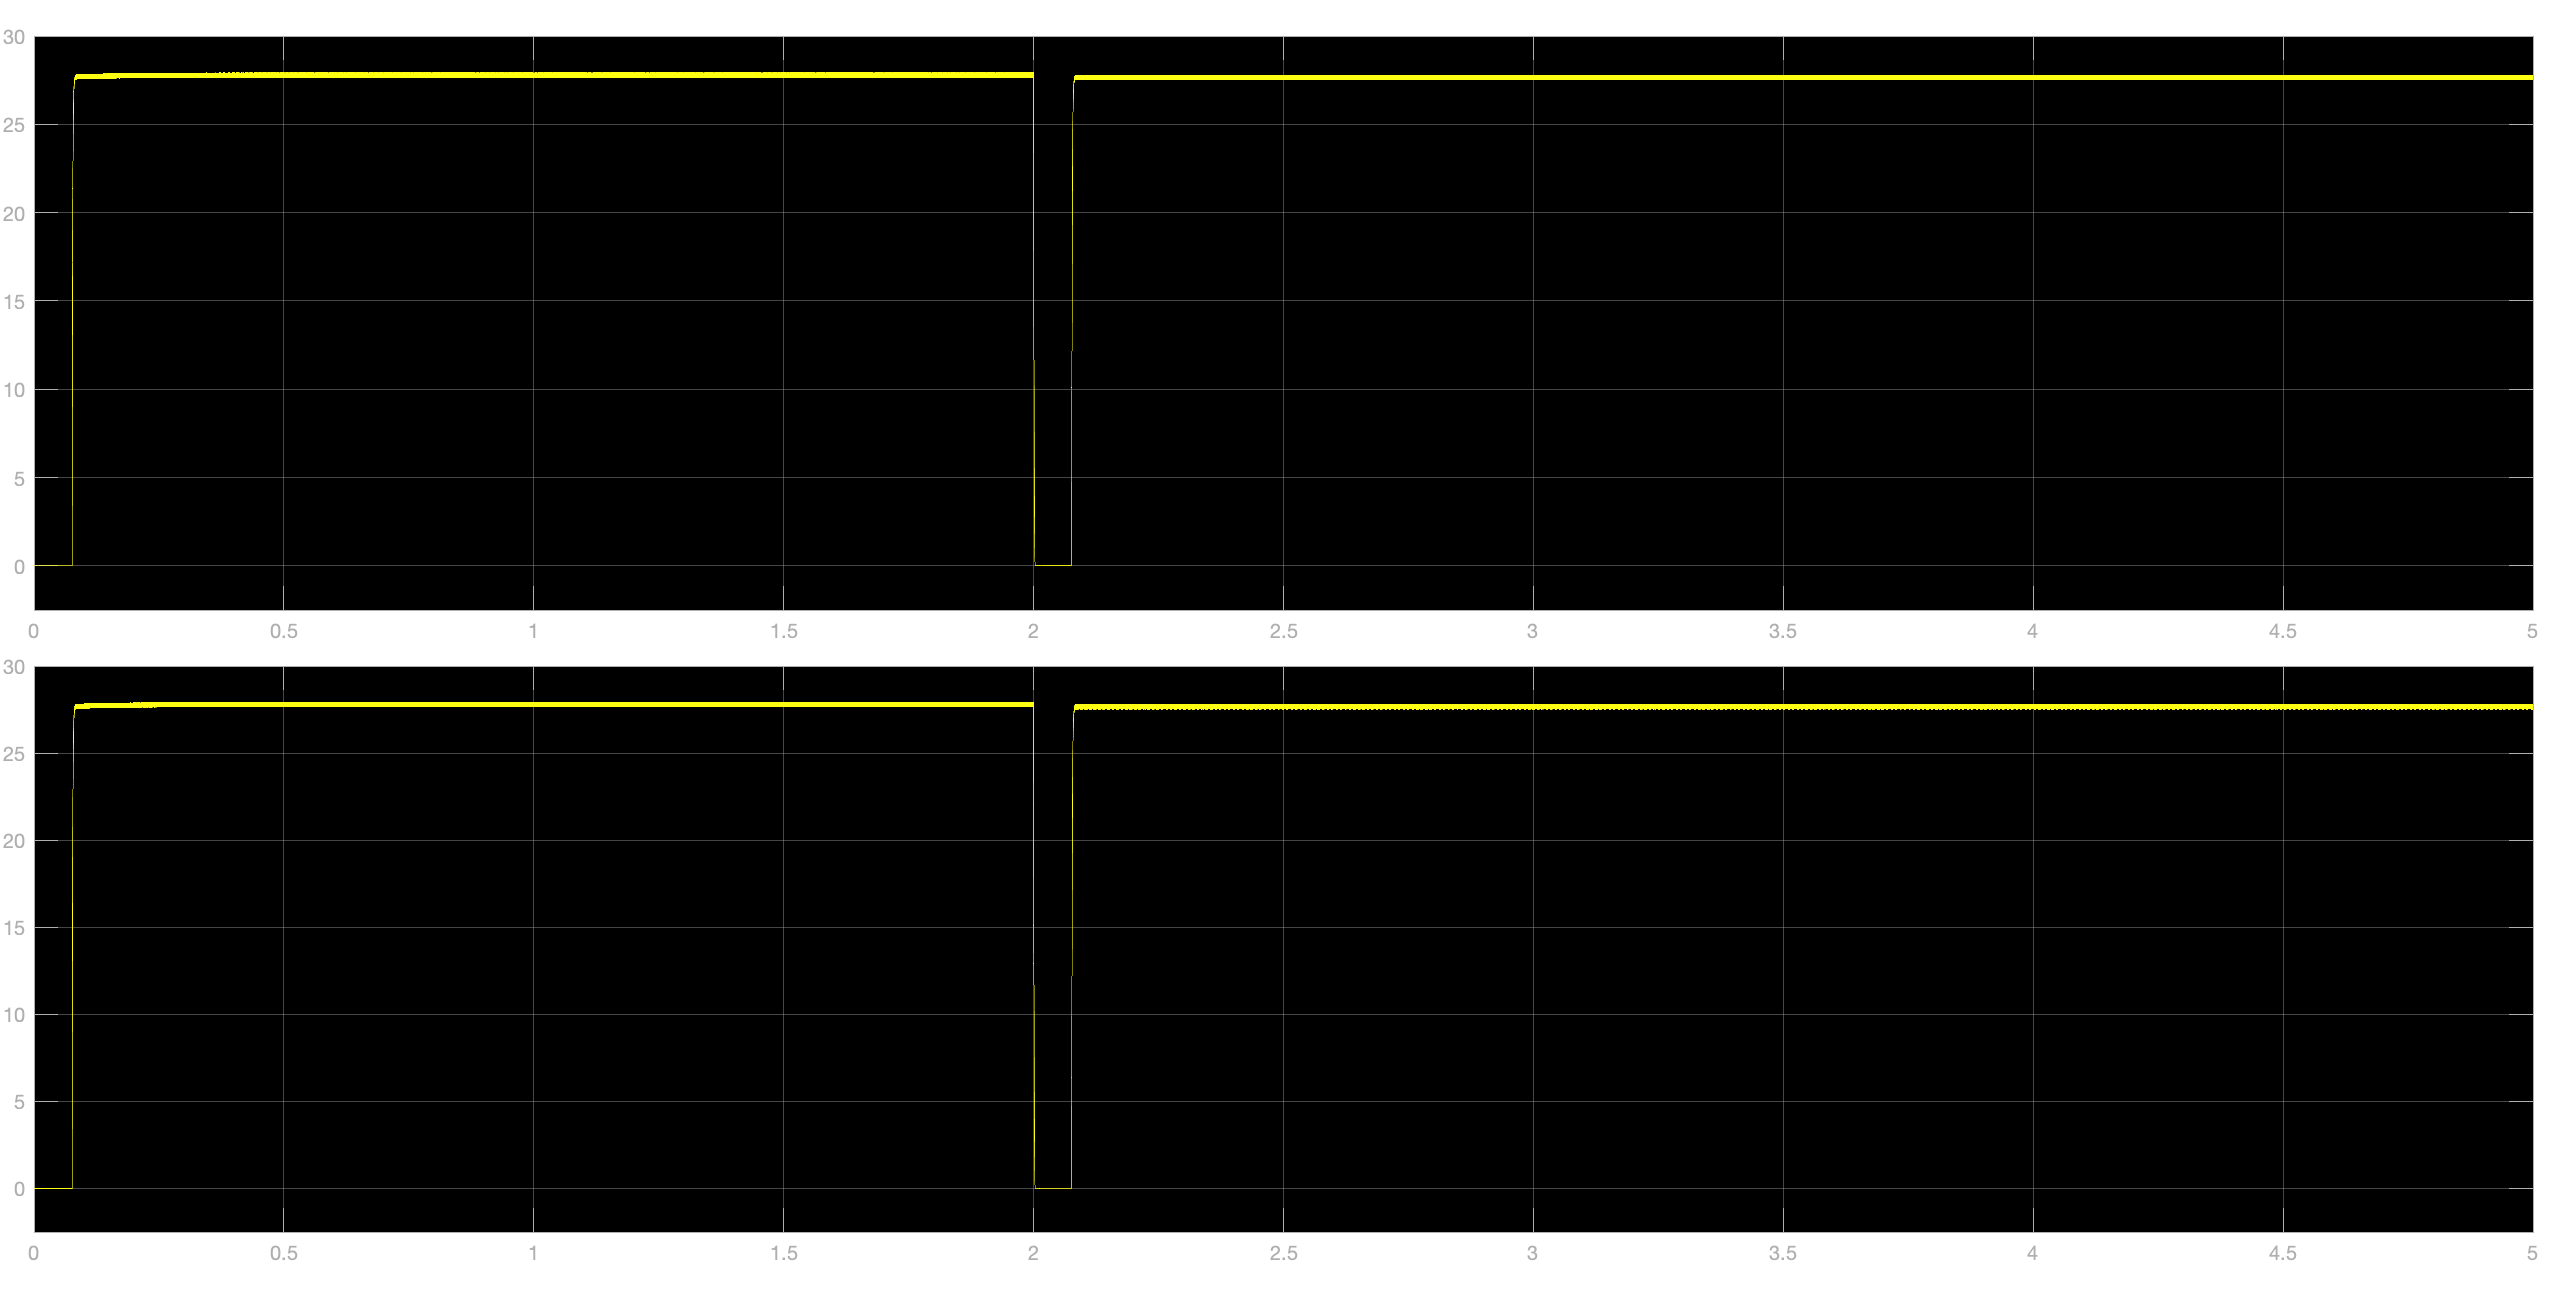
\includegraphics{gl_gr_ar_load2.png}}
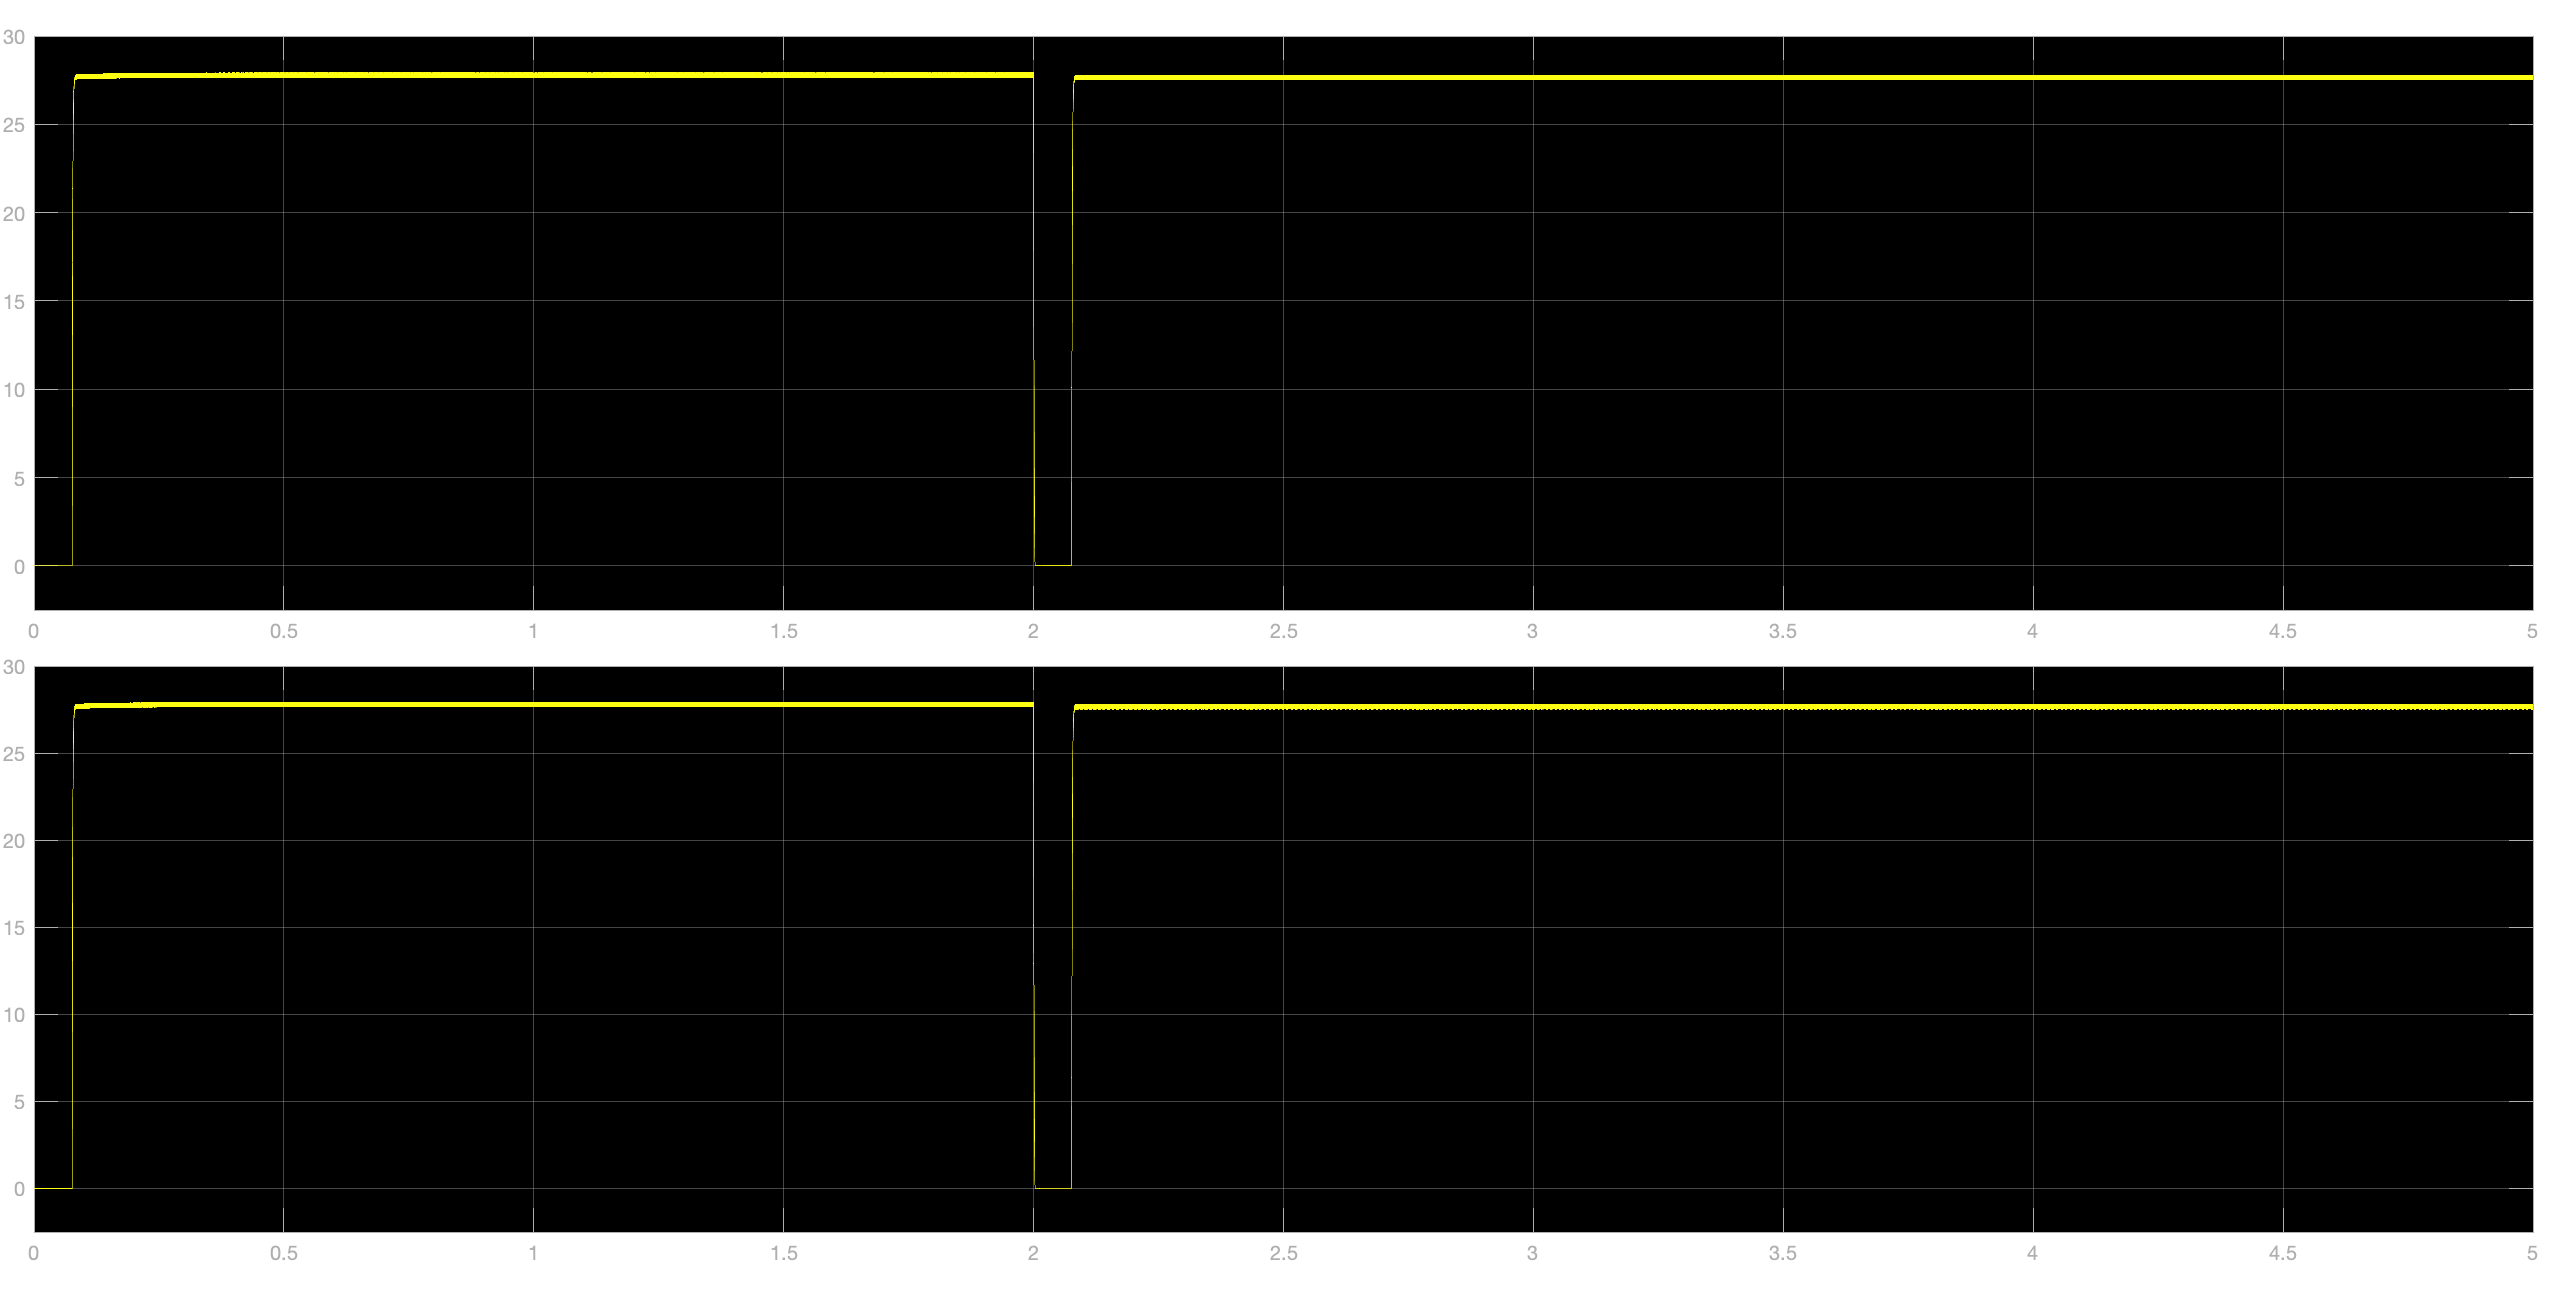
\includegraphics[trim= 0 0.255\imageheight{} 0 0, clip, width = 0.185\imageheight{}]{gl_gr_ar_load2.png}
\begin{center}
\small{Figure 2.8.2 Right DC Load Waveform}
\end{center}
\begin{center}
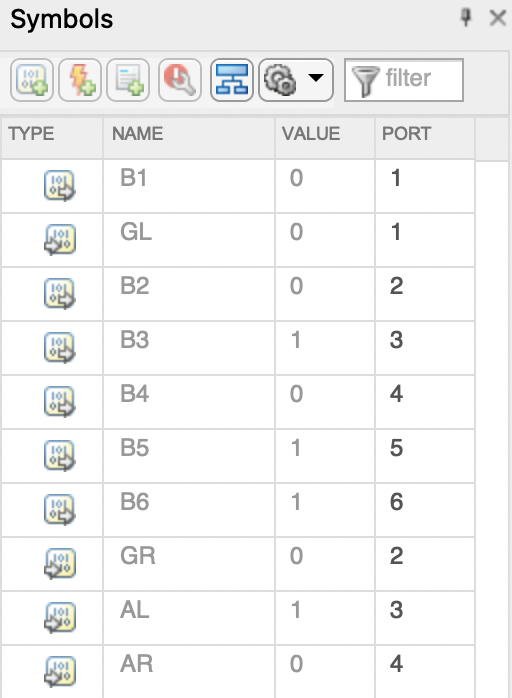
\includegraphics[width=4.5cm]{gl_gr_ar_signals.png}
\end{center}
\begin{center}
\small{Figure 2.8.3 BPCU Output Control Signals}
\end{center}
\begin{center}
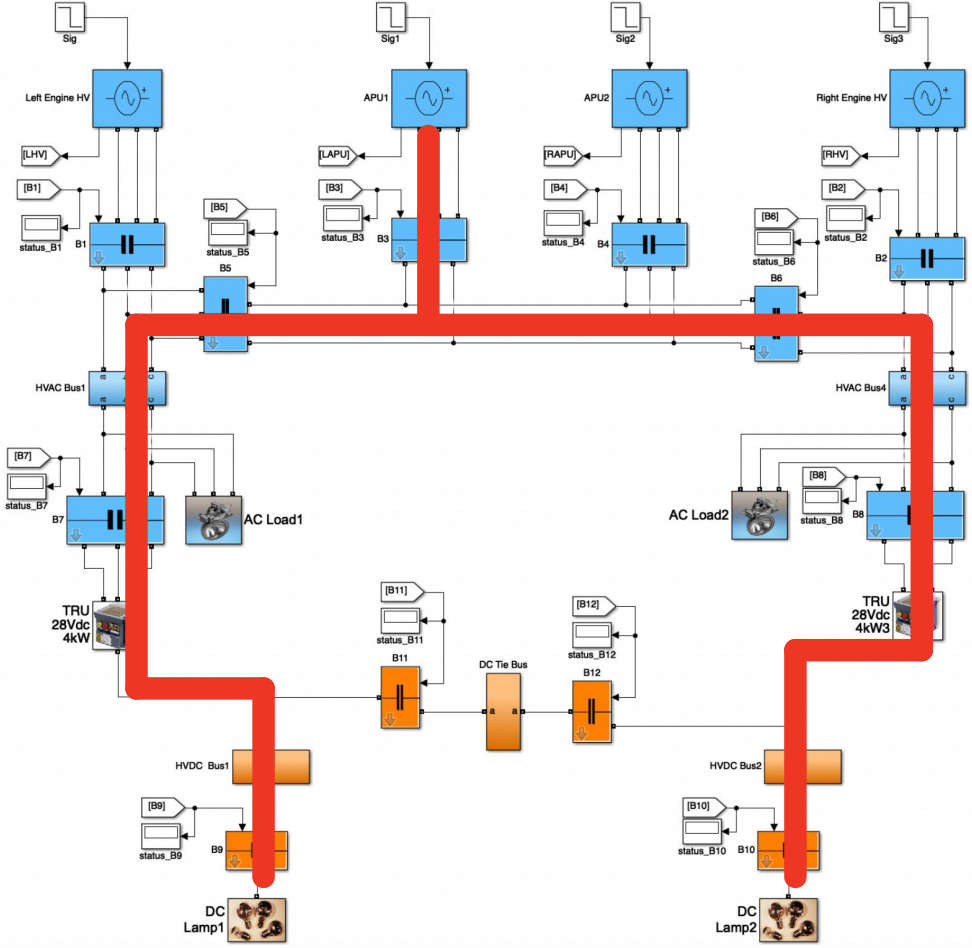
\includegraphics[width=14.5cm]{gl_gr_ar.png}
\end{center}
\begin{center}
\small{Figure 2.8.4 EPS Connection}
\end{center}
When GR, GL,  and AR fail,  the only power supply left, AL, is inserted into the network and empowers both AC buses based on system guarantee G4, G7, and G8.
\pagebreak

\subsection{Case 8: GR, GL, AL Not Working}
\settowidth{\imageheight}{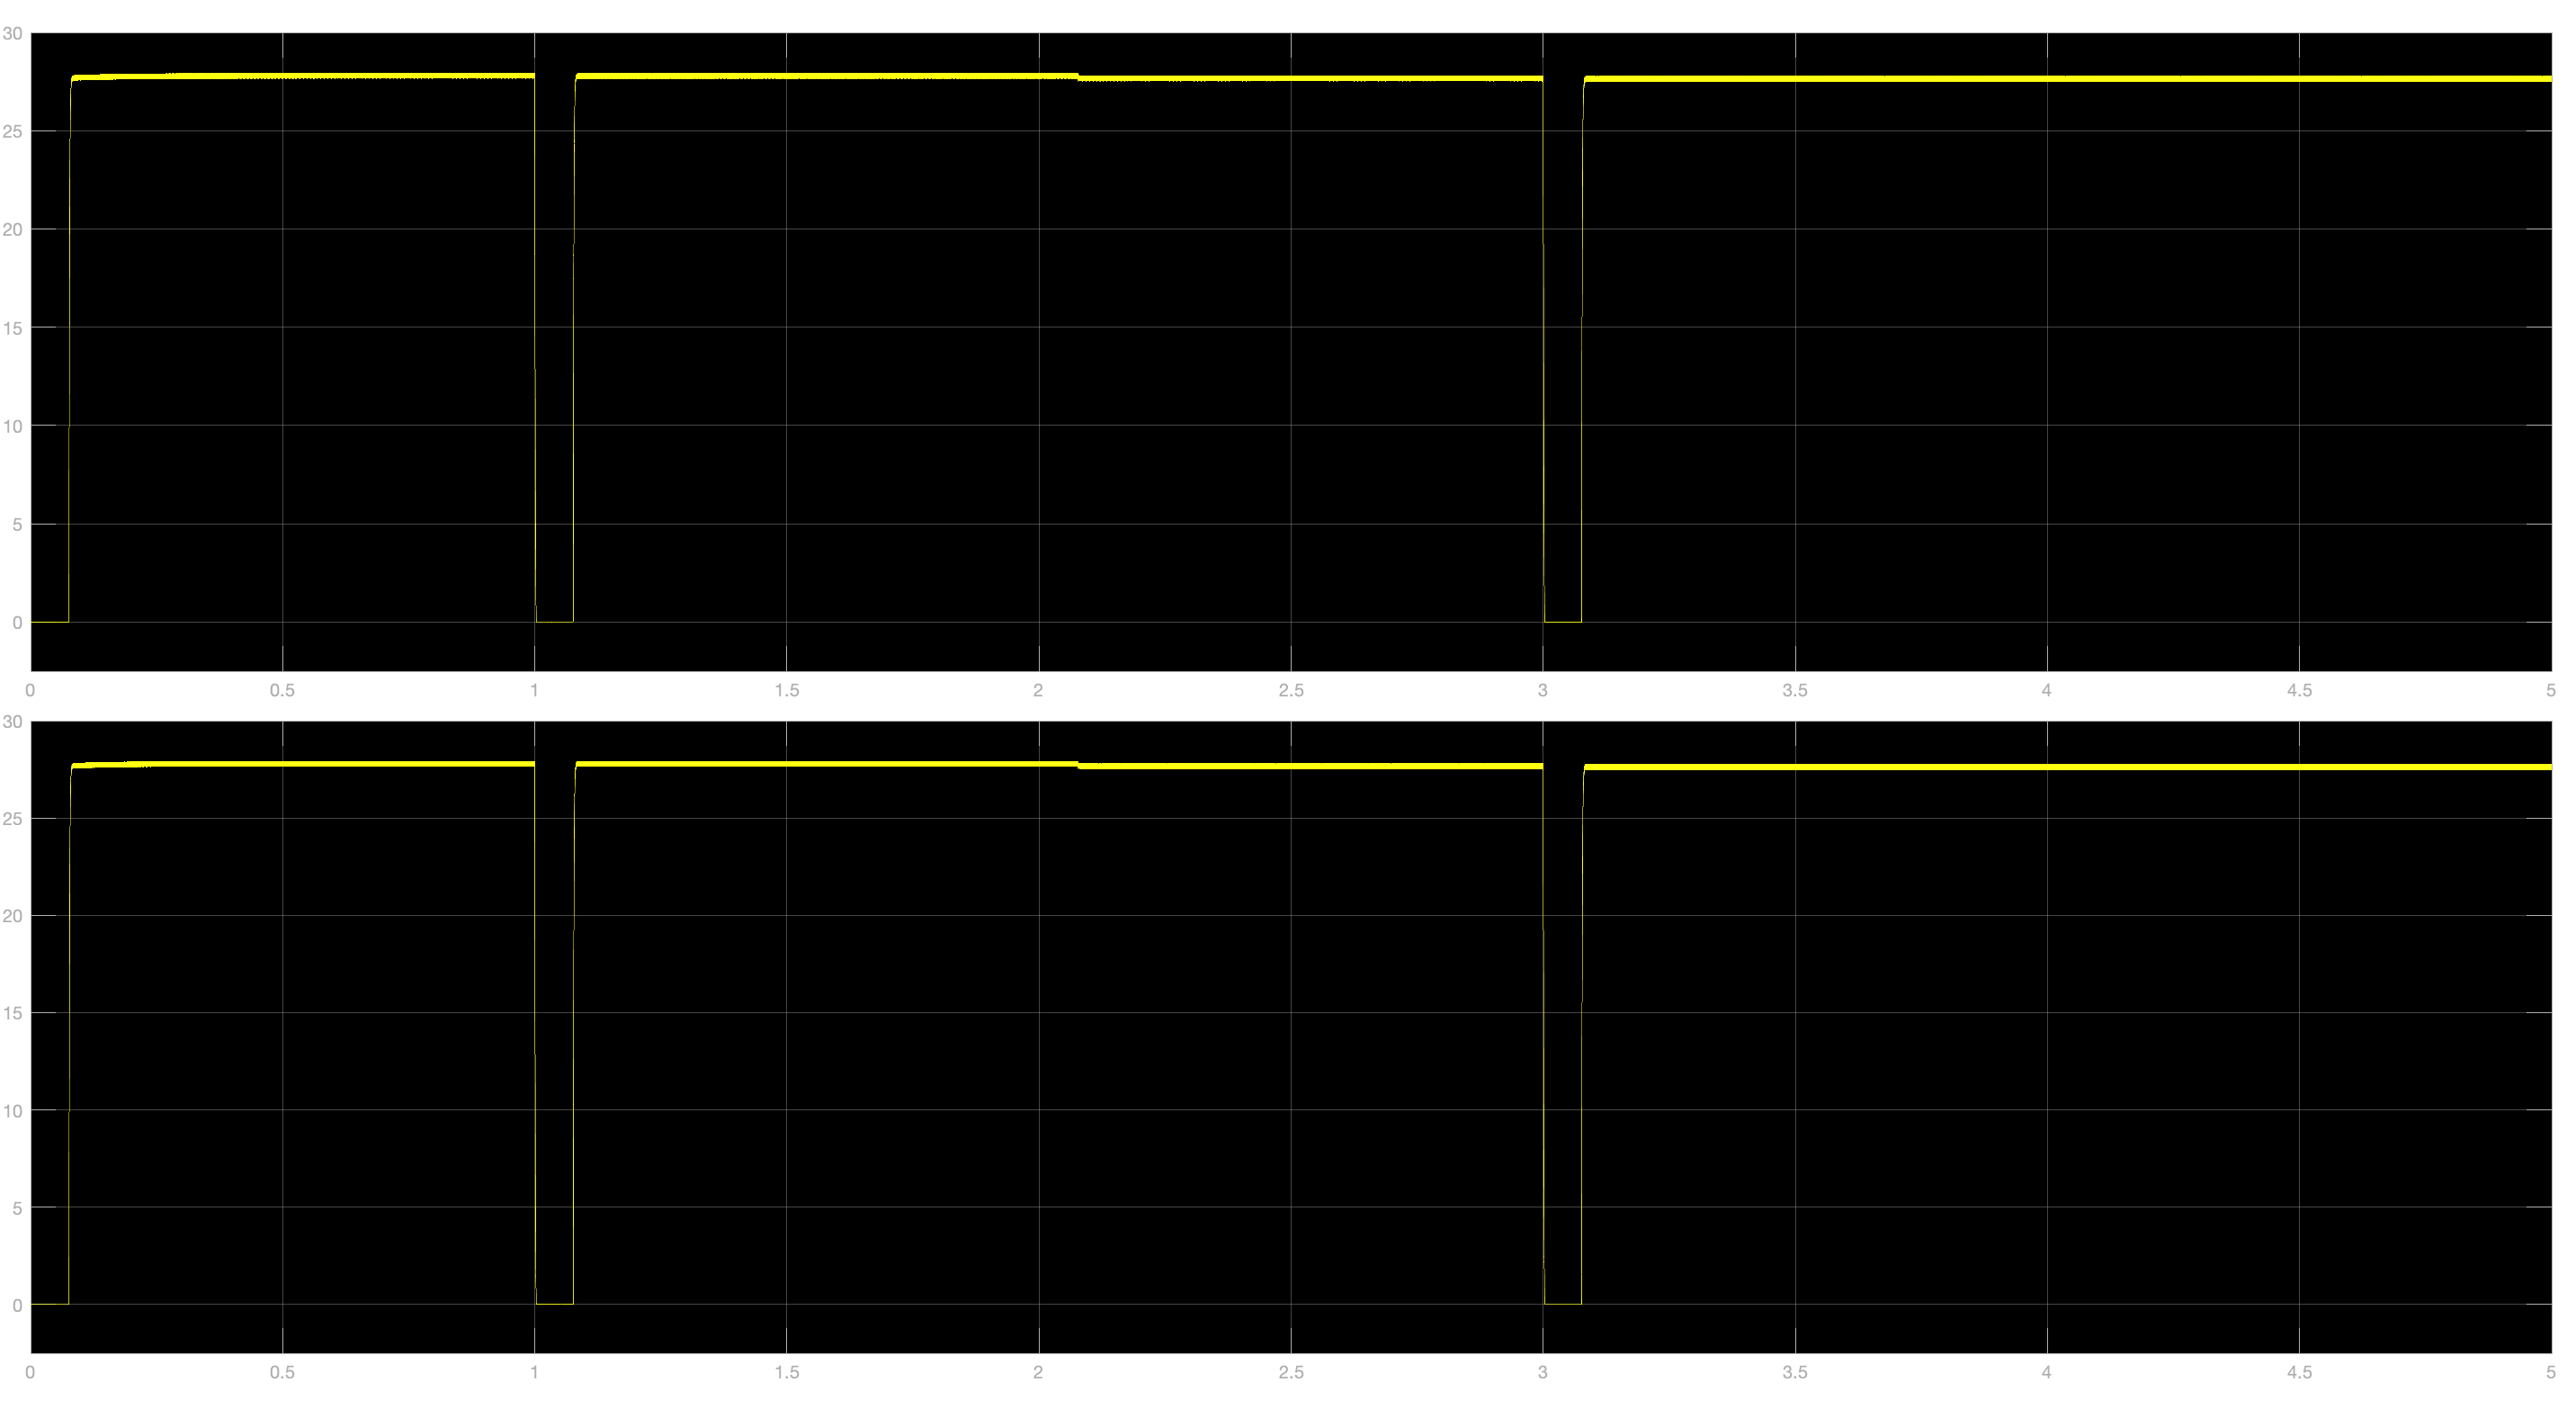
\includegraphics{gl_gr_al_load1.png}}
\begin{center}
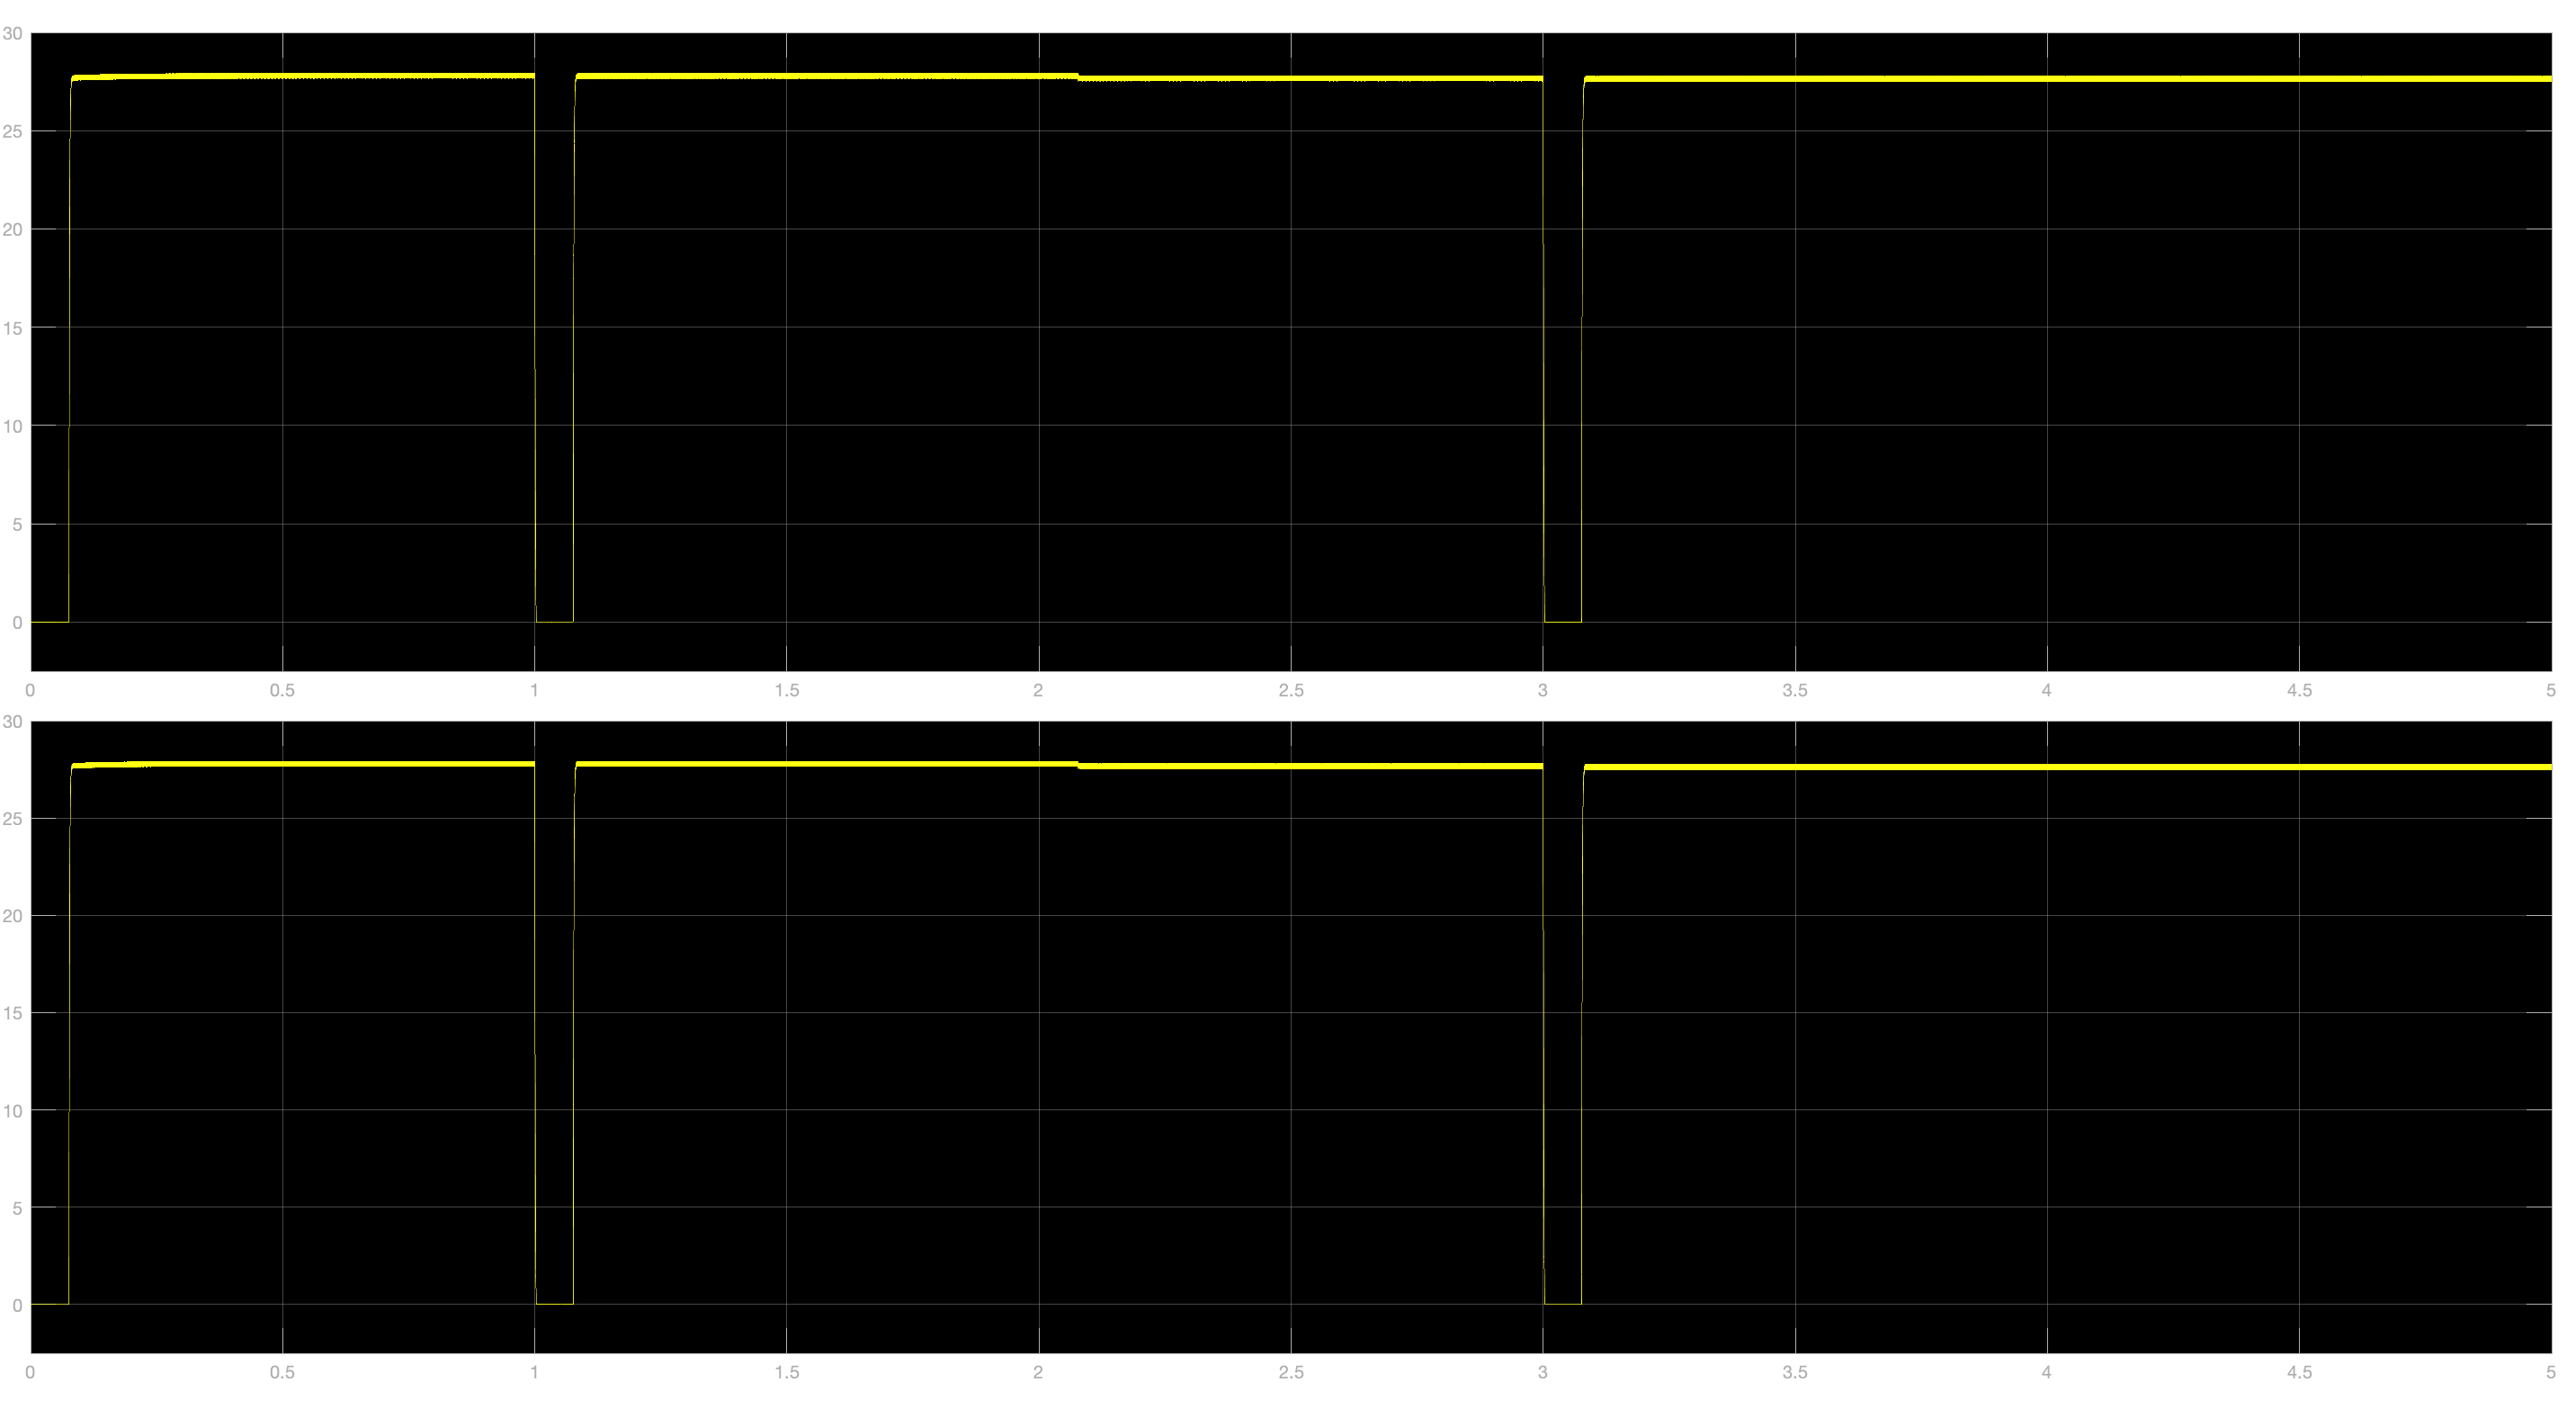
\includegraphics[trim= 0 0.28\imageheight{} 0 0, clip, width = 0.165\imageheight{}]{gl_gr_al_load1.png}
\end{center}
\begin{center}
\small{Figure 2.9.1 Left DC Load Waveform}
\end{center}
\settowidth{\imageheight}{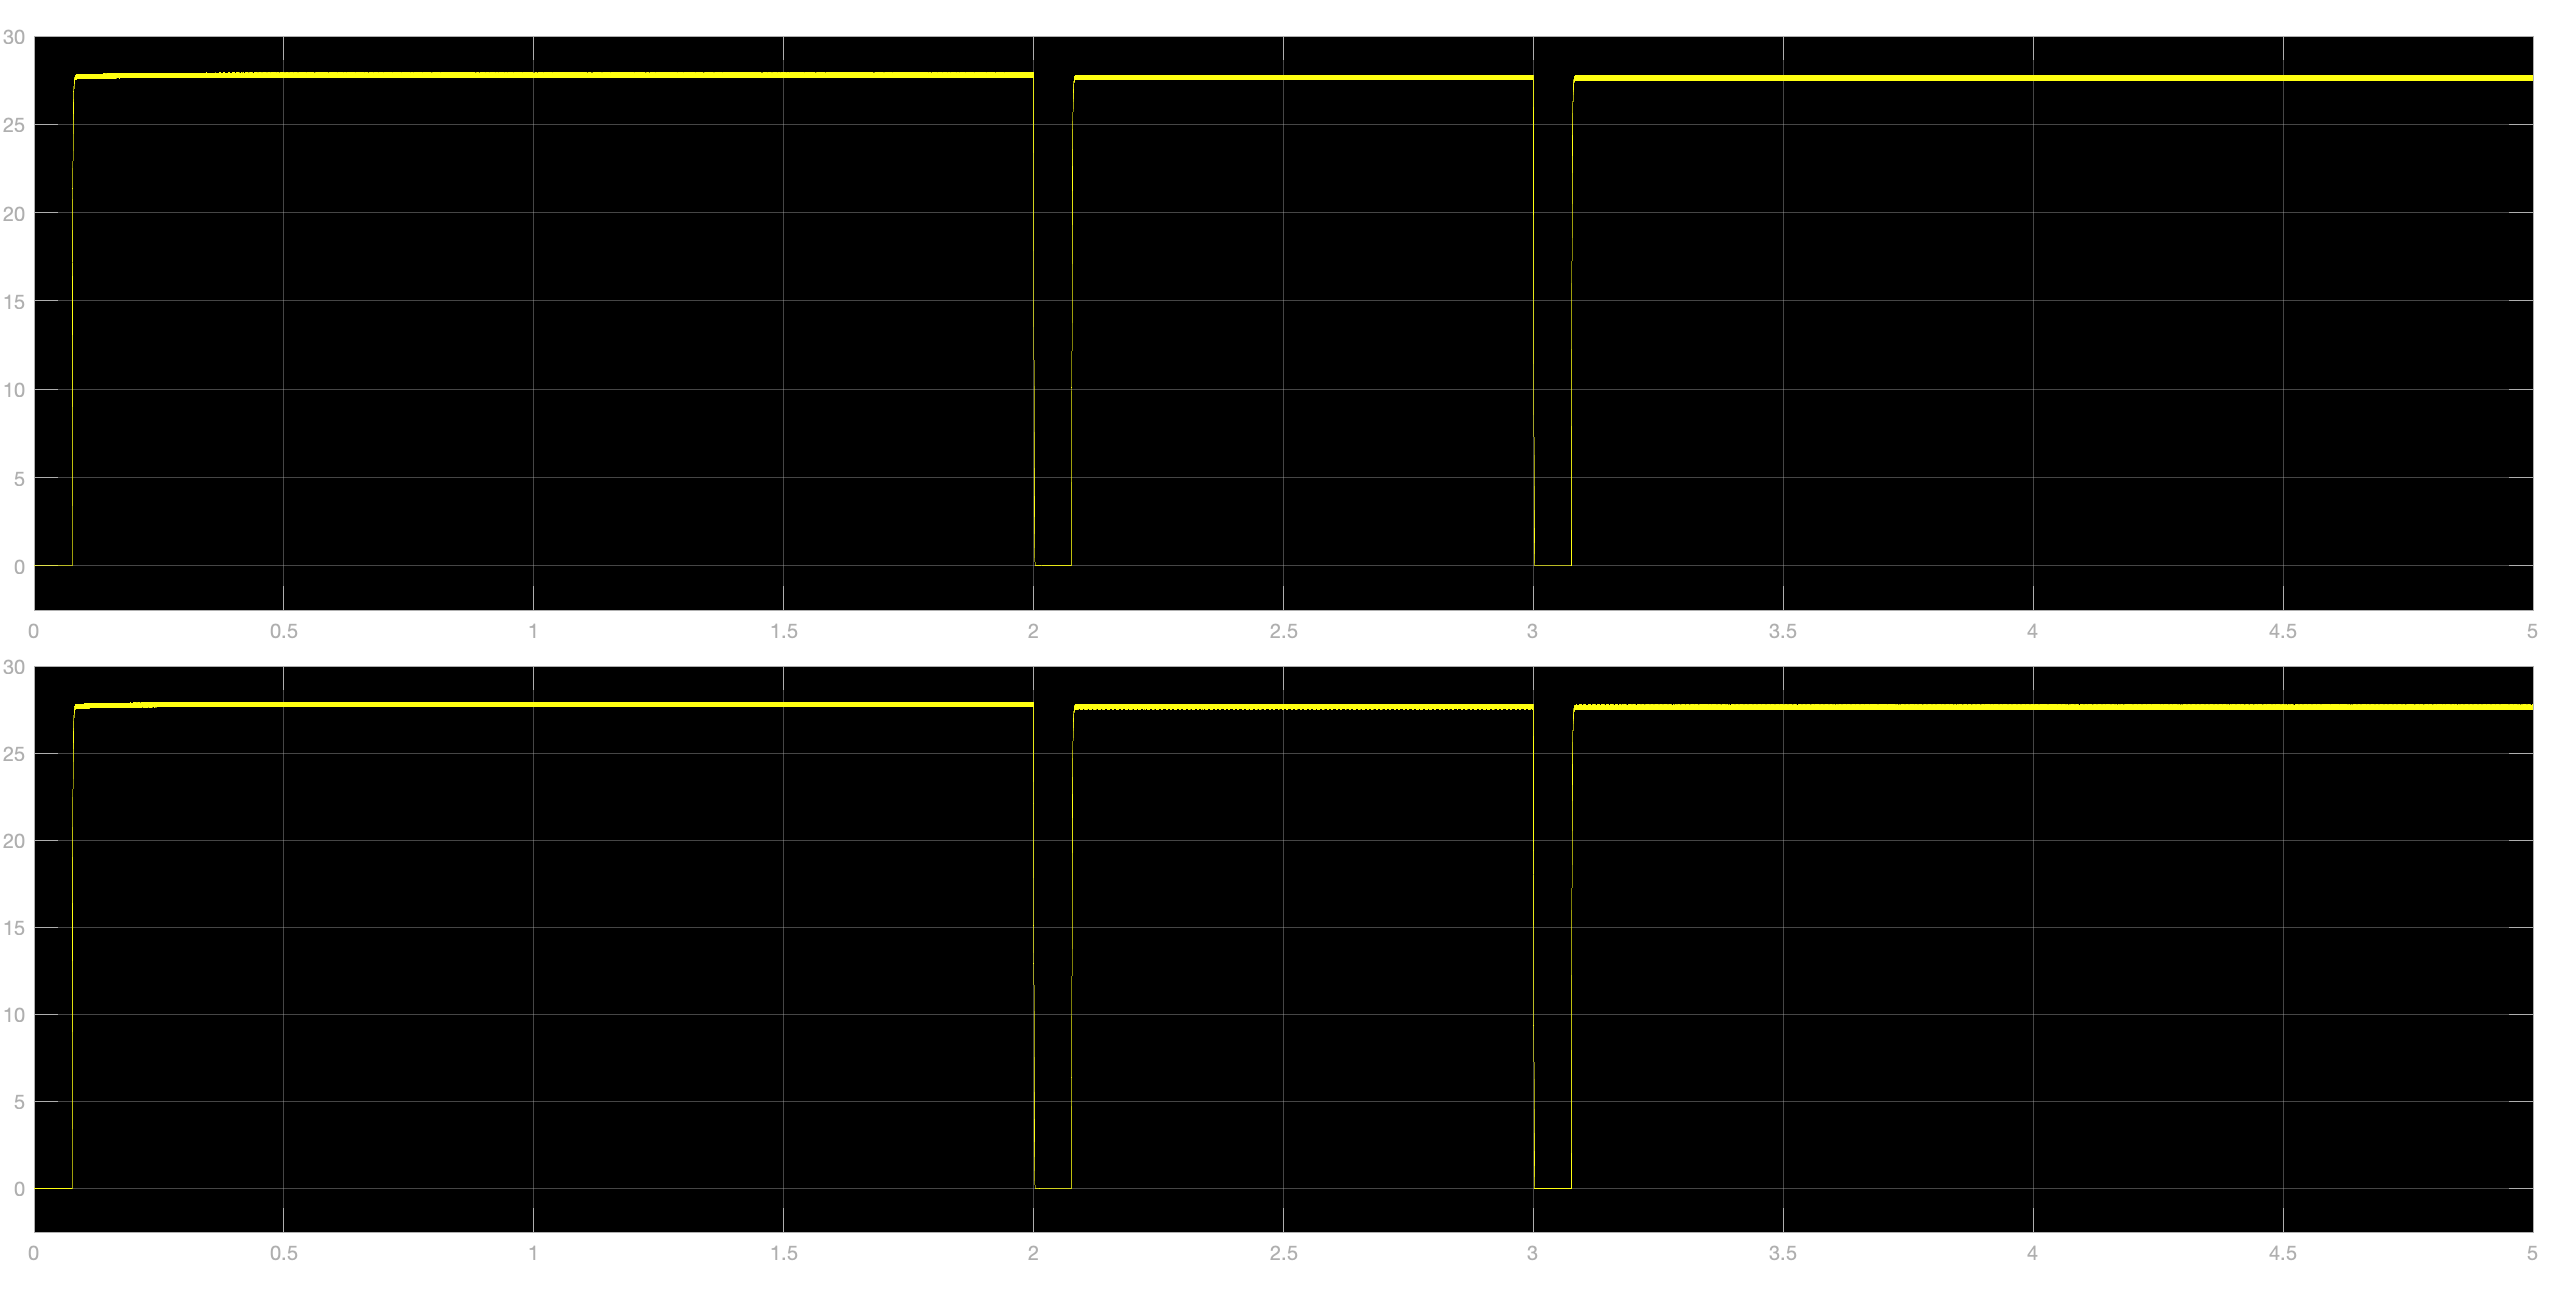
\includegraphics{gl_gr_al_load2.png}}
\includegraphics[trim= 0 0.255\imageheight{} 0 0, clip, width = 0.185\imageheight{}]{gl_gr_al_load2.png}
\begin{center}
\small{Figure 2.9.2 Right DC Load Waveform}
\end{center}
\begin{center}
\includegraphics[width=4.5cm]{gl_gr_al_signals.png}
\end{center}
\begin{center}
\small{Figure 2.9.3 BPCU Output Control Signals}
\end{center}
\begin{center}
\includegraphics[width=14.5cm]{gl_gr_al.png}
\end{center}
\begin{center}
\small{Figure 2.9.4 EPS Connection}
\end{center}
When GR, GL,  and AL fail,  the only power supply left, AR, is inserted into the network and empowers both AC buses based on system guarantee G4, G7, and G8.
\pagebreak

\subsection{Case 9: GR, AR, AL Not Working}
\settowidth{\imageheight}{\includegraphics{gr_ar_al_load1.png}}
\begin{center}
\includegraphics[trim= 0 0.28\imageheight{} 0 0, clip, width = 0.165\imageheight{}]{gr_ar_al_load1.png}
\end{center}
\begin{center}
\small{Figure 2.10.1 Left DC Load Waveform}
\end{center}
\settowidth{\imageheight}{\includegraphics{gr_ar_al_load2.png}}
\includegraphics[trim= 0 0.255\imageheight{} 0 0, clip, width = 0.185\imageheight{}]{gr_ar_al_load2.png}
\begin{center}
\small{Figure 2.10.2 Right DC Load Waveform}
\end{center}
\begin{center}
\includegraphics[width=4.5cm]{gr_ar_al_signals.png}
\end{center}
\begin{center}
\small{Figure 2.10.3 BPCU Output Control Signals}
\end{center}
\begin{center}
\includegraphics[width=14.5cm]{gr_ar_al.png}
\end{center}
\begin{center}
\small{Figure 2.10.4 EPS Connection}
\end{center}
When GR, AR,  and AL fail,  the only power supply left, GL, is inserted into the network and empowers both AC buses based on system guarantee G7 and G8.
\pagebreak

\subsection{Case 10: GL, AR, AL Not Working}
\settowidth{\imageheight}{\includegraphics{gl_ar_al_load1.png}}
\begin{center}
\includegraphics[trim= 0 0.28\imageheight{} 0 0, clip, width = 0.165\imageheight{}]{gl_ar_al_load1.png}
\end{center}
\begin{center}
\small{Figure 2.11.1 Left DC Load Waveform}
\end{center}
\settowidth{\imageheight}{\includegraphics{gl_ar_al_load2.png}}
\includegraphics[trim= 0 0.255\imageheight{} 0 0, clip, width = 0.185\imageheight{}]{gl_ar_al_load2.png}
\begin{center}
\small{Figure 2.11.2 Right DC Load Waveform}
\end{center}
\begin{center}
\includegraphics[width=4.5cm]{gl_ar_al_signals.png}
\end{center}
\begin{center}
\small{Figure 2.11.3 BPCU Output Control Signals}
\end{center}
\begin{center}
\includegraphics[width=14.5cm]{gl_ar_al.png}
\end{center}
\begin{center}
\small{Figure 2.11.4 EPS Connection}
\end{center}
When GL, AR,  and AL fail,  the only power supply left, GR, is inserted into the network and empowers both AC buses based on system guarantee G7 and G8.
\pagebreak

\section{Learning Experience with Simulink}
The learning experience with Simulink was time-consuming but satisfactory for us. We self-studied how to build control logic with Stateflow toolbox, how to generate and observe digital waveforms, and how to write and run tests for simulation. In addition, we improved our time management ability, learned how to cooperate well within the team, and experienced with a lot of Simulink trouble-shooting and debugging. The characteristics of Simulink that we like most are its graphical user interface that is friendly for beginners and its large number of built-in functions, waveforms, and modules within Simulink libraries. However, Simulink is not intelligent enough, for example, we have to mannually choose correct input and output ports for variables, which might cause a lot of confusion because the variables and ports are not automatically paired. This is the aspect that we dislike most.



\end{document}

%% 
%% This work consists of these files mcmthesis.dtx,
%%                                   figures/ and
%%                                   code/,
%% and the derived files             mcmthesis.cls,
%%                                   mcmthesis-demo.tex,
%%                                   README,
%%                                   LICENSE,
%%                                   mcmthesis.pdf and
%%                                   mcmthesis-demo.pdf.
%%
%% End of file `mcmthesis-demo.tex'.
